\documentclass[12pt,a4paper]{article}

% Paquetes básicos
\usepackage[x11names]{xcolor}
\usepackage[utf8]{inputenc}
\usepackage{mathtools, amssymb, amsthm}
\usepackage{changepage}
\usepackage{geometry}
\usepackage[colorlinks=true]{hyperref}
\usepackage{enumitem}
\usepackage{etoolbox}
\usepackage{graphicx}
\usepackage{setspace}
\usepackage{tcolorbox}
\tcbuselibrary{skins, breakable}
\usepackage{titlesec}
\usepackage{tikz} % core TikZ
\usetikzlibrary{matrix}
\usepackage{pgfplots}
\pgfplotsset{compat=newest}
\usepgfplotslibrary{fillbetween}

% Margins
%\geometry{left=3cm,right=3cm,top=2.5cm,bottom=2.5cm}

% Custom operators
\newcommand{\card}{\operatorname{card}}
\newcommand{\muae}{\overset{\mu-a.e.}{=}}

% Implication box setup
\tcbset{Implication-number/.style={
  enhanced,
  boxsep=2pt,
  colback=white,
  frame hidden,
  sharp corners,
  left=2pt, right=2pt, top=1pt, bottom=1pt,
  underlay={
    \draw[line width=0.5pt] (frame.south west) -- ([xshift=-133mm]frame.south east); % línea horizontal
    \draw[line width=0.5pt] ([xshift=-133mm]frame.north east) -- ([xshift=-133mm]frame.south east); % línea vertical
  }
}}

\tcbset{Implication-number-ds/.style={
  enhanced,
  boxsep=2pt,
  colback=white,
  frame hidden,
  sharp corners,
  left=2pt, right=2pt, top=1pt, bottom=1pt,
  underlay={
    \draw[line width=0.5pt] ([yshift=5mm]frame.south west) -- ([xshift=-133mm, yshift=5mm]frame.south east); % línea horizontal
    \draw[line width=0.5pt] ([xshift=-133mm, yshift=-3mm]frame.north east) -- ([xshift=-133mm, yshift=5mm]frame.south east); % línea vertical
  }
}}

\tcbset{Subset-contingency/.style={
  enhanced,
  boxsep=2pt,
  colback=white,
  frame hidden,
  sharp corners,
  left=2pt, right=2pt, top=1pt, bottom=1pt,
  underlay={
    \draw[line width=0.5pt] (frame.south west) -- ([xshift=-140mm]frame.south east); % línea horizontal
    \draw[line width=0.5pt] ([xshift=-140mm]frame.north east) -- ([xshift=-140mm]frame.south east); % línea vertical
  }
}}

\tcbset{Indent-subset-contingency/.style={
  enhanced,
  boxsep=2pt,
  colback=white,
  frame hidden,
  sharp corners,
  left=2pt, right=2pt, top=1pt, bottom=1pt,
  underlay={
    \draw[line width=0.5pt] (frame.south west) -- ([xshift=-140mm+0.07\textwidth]frame.south east); % línea horizontal
    \draw[line width=0.5pt] ([xshift=-140mm+0.07\textwidth]frame.north east) -- ([xshift=-140mm+0.07\textwidth]frame.south east); % línea vertical
  }
}}

% Useful commands
\renewcommand{\contentsname}{Contenidos}

\newcommand{\R}{\mathbb{R}}
\newcommand{\N}{\mathbb{N}}
\newcommand{\Z}{\mathbb{Z}}
\newcommand{\Q}{\mathbb{Q}}
\newcommand{\C}{\mathbb{C}}

\newcommand{\smallcup}{\mathop{\cup}\limits}
\newcommand{\smallcap}{\mathop{\cap}\limits}
\newcommand{\smallsum}{\mathop{\sum}\limits}
\newcommand{\smallprod}{\mathop{\prod}\limits}

\newcommand{\linf}[1]{\displaystyle{\mathop{\underline{\lim}}_{#1}}}
\newcommand{\mlim}[1]{\displaystyle{\lim_{#1}}}

%Integral de Lebesgue con patas
\newcommand{\lbint}{\mathop{\int_{\!\!\!\!\!|\!}^{\!|\!}}}

%Espacios \mathcal{L}_p
\newcommand{\elep}[2]{\mathcal{L}_{#1}(#2)}

% ----- Custom counters and counter commands -----
% Custom counter hierarchy
\newcounter{unit}[section]
\newcounter{chapter}[unit]
\makeatletter
\@addtoreset{subsubsection}{chapter}
\makeatother

\renewcommand{\theunit}{\arabic{unit}}
\renewcommand{\thechapter}{\arabic{chapter}}
\renewcommand{\thesubsubsection}{\theunit.\thechapter.\arabic{subsubsection}}

% Custom content hierarchy behavior
\newcommand{\chapter}[1]{
    \refstepcounter{chapter}
    \subsection*{\Large{\S \thechapter. #1}}
    \addcontentsline{toc}{subsection}{\thechapter. #1}
}
\newcommand{\unit}[1]{
    \refstepcounter{unit}
    \section*{\Huge{\Roman{unit} #1}}
    \addcontentsline{toc}{section}{\Roman{unit} #1}
}

\newcommand{\result}[1]{%
  \subsubsection{#1}%
  \label{result:\thesubsubsection}
}
  
\titleformat{\subsubsection}
    {\normalfont\large\bfseries} % mismo tamaño que \subsection
    {\thesubsubsection}{1em}{}
  
%---- Custom proof commands-----
\newcommand{\dem}{
    \noindent \underline{\textbf{Demostración:}}
}
\newcommand{\nota}{
    \noindent \underline{\textbf{Nota:}}
}
% ----------------------------------------
\hbadness=10000
\vbadness=10000
\hfuzz=100pt
\vfuzz=100pt
% ---------------------------------------
\title{Análisis Matemático III}
\author{Javier Ortín Rodenas}
\date{Curso 2025-2026}


\begin{document}

\maketitle
\newpage
\hypersetup{linkcolor=black}
\tableofcontents
\hypersetup{linkcolor=Ivory4}
\newpage

\section*{\Huge{Introducción de la asignatura}}
\hspace{3mm}
\begin{onehalfspace}
La materia será la misma que en años anteriores, aunque habrá un cambio en la metodología de enseñanza: no habrá tutorías grupales. No obstante, sí habrá evaluación continua. Su funcionamiento se explicará posteriormente.

%TODO: placeholder for evaluación continua

\newpage

\section*{\Huge{Preliminares}}
\phantomsection \addcontentsline{toc}{section}{Preliminares}
En la sección de preliminares se tratarán los siguientes temas:
\begin{itemize}
    \item Cardinalidad de conjuntos
    \item Descomposición de abiertos de $\R^N$ en unión de cubos diádicos
    \item Series dobles
\end{itemize}

\vspace{2mm}

\chapter{Cardinalidad de conjuntos}

\vspace{2mm}

\result{Definición de cardinalidad, tipos de cardinalidad}
\hspace{3mm}
Intuitivamente, podemos definir la cardinalidad de un conjunto como el número de elementos que tiene. Además, es lógico plantear la distinción entre conjuntos finitos e infinitos. Veamos cómo formalizar esta idea.

\vspace{2mm}

Sea $A$ un conjunto no vacío, diremos que $A$ es un conjunto finito de cardinalidad $n \in \N = \{1,2,\ldots\}$ si existe una aplicación biyectiva $\varphi : \{1,2,\ldots,n\} \to A$.

\noindent Se considera que el conjunto vacío $\varnothing$ es finito con cardinal $0$.

\vspace{4mm}

Sea $A$ un conjunto cualquiera, diremos que es un conjunto infinito si existe cierta aplicación inyectiva $\varphi : \N \to A$. Dentro de esta clasificación, diremos que $A$ es infinito numerable si existe una aplicación $\varphi : \N \to A$ biyectiva. Si esto último no fuese posible, diremos que $A$ es infinito no numerable.

\vspace{4mm}

Aunque no entra dentro de los objetivos de esta asignatura, es interesante contemplar la siguiente observación: Si un conjunto no es un conjunto finito, podemos afirmar simplemente que es un conjunto ``no finito''. Si además incluimos el axioma de elección, sí podremos afirmar que tal conjunto es infinito. Dentro de los conjuntos infinitos, todos son o bien numerables o bien no numerables, sin intersección entre ambas categorías.

\vspace{4mm}

\result{Ejemplos de conjuntos numerables}

$\bullet$ $\N$: trivial, basta considerar la aplicación identidad. \\

\noindent
$\bullet$ $\Z$: basta considerar la siguiente aplicación biyectiva:

%Function definition and mapping side by side
\begin{minipage}{0.5\textwidth}
    \begin{align*}
    \varphi(n) =
    \begin{cases}
    \frac{n}{2}, & \text{si } n \text{ es par} \\
    -\frac{n-1}{2}, & \text{si } n \text{ es impar}
    \end{cases}
    \end{align*}
\end{minipage}%
\begin{minipage}{0.5\textwidth}
    \begin{align*}
    \begin{array}{cccccc}
    1 & 2 & 3 & 4 & 5 & \cdots \\
    \downarrow\!\varphi & \downarrow\!\varphi & \downarrow\!\varphi & \downarrow\!\varphi & \downarrow\!\varphi & \\
    0 & 1 & -1 & 2 & -2 & \cdots
    \end{array}
    \end{align*}
\end{minipage}

\vspace{7mm}

\noindent $\bullet$ $\Q := \left\{\frac{z}{n} : z \in \Z, n \in \N \right\}$. Denotaremos por $\hat{Q}$ al conjunto $\left\{\frac{z}{n} : z,n \in \N\right\}$. Como hemos visto en el apartado anterior, al ser $\Z$ numerable, $\hat{Q}$ y $\Q$ han de tener necesariamente la misma cardinalidad. Por tanto, basta con demostrar que $\hat{Q}$ es numerable, lo que haremos a continuación por medio de una doble desigualdad.

\vspace{2mm}

\phantomsection \label{racionales-numerables}
Representaremos los elementos de $\hat{Q}$ en una tabla infinita que recorreremos diagonalmente:
\begin{center}
    \scalebox{0.9}{ %downscale the tikzpicture
    \begin{tikzpicture}[baseline=(current bounding box.center)]
    % Draw the table with extra space for lines
    \matrix (m) [matrix of math nodes, nodes in empty cells, row sep=8mm, column sep=10mm, ampersand replacement=\&, cells={nodes={minimum width=1.5em, minimum height=2.5ex, anchor=center, text height=1.5ex, text depth=.25ex}} ]{
    {} \& 1 \& 2 \& 3 \& 4 \& \ldots \\
    1 \& \frac{1}{1} \& \frac{2}{1} \& \frac{3}{1} \& \frac{4}{1} \& \ldots \\
    2 \& \frac{1}{2} \& \frac{2}{2} \& \frac{3}{2} \& \frac{4}{2} \& \ldots \\
    3 \& \frac{1}{3} \& \frac{2}{3} \& \frac{3}{3} \& \frac{4}{3} \& \ldots \\
    4 \& \frac{1}{4} \& \frac{2}{4} \& \frac{3}{4} \& \frac{4}{4} \& \ldots \\
    \vdots \& \vdots \& \vdots \& \vdots \& \vdots \& \ddots \\
    };
    % Draw horizontal line below header row
    \draw[thick] ([xshift=-4mm, yshift=-2mm]m-1-1.south west) -- ([xshift=7mm, yshift = -2mm]m-1-6.south east);
    % Draw vertical line after header column
    \draw[thick] ([xshift =4mm ,yshift=5mm]m-1-1.north east) -- ([xshift=4mm, yshift=-5mm]m-6-1.south east);

    % Draw diagonal arrows
    \draw[->, thick, red] ([xshift=2mm, yshift=2mm]m-2-2.north east) -- (m-2-2) -- ([xshift=-2mm, yshift=-2mm]m-2-2.south west); % 1st diagonal (1/1
    \draw[->, thick, red] ([xshift=2mm, yshift=2mm]m-2-3.north east) --(m-2-3) -- (m-3-2) -- ([xshift=-2mm, yshift=-2mm]m-3-2.south west); % 2nd diagonal (2/1 to 1/2)
    \draw[->, thick, red] ([xshift=2mm, yshift=2mm]m-2-4.north east) --(m-2-4) -- (m-3-3) -- (m-4-2) -- ([xshift=-2mm, yshift=-2mm]m-4-2.south west) ; % 3rd diagonal (3/1 to 1/3)
    \draw[->, thick, red] ([xshift=2mm, yshift=2mm]m-2-5.north east) -- (m-2-5) -- (m-3-4) -- (m-4-3) -- (m-5-2)-- ([xshift=-2mm, yshift=-2mm]m-5-2.south west); % 4th diagonal (4/1 to 1/4)

    % Add more diagonals if needed
    \end{tikzpicture}
    }
\end{center}
Por tanto, obtenemos como resultado la siguiente aplicación
$\varphi : \N \to \hat{Q}$ con
$$\varphi(1) = \frac{1}{1}, \hspace{4mm} \varphi(2) = \frac{2}{1}, \hspace{4mm}
\varphi(3) = \frac{1}{2},  \hspace{4mm} \varphi(4) = \frac{3}{1}, \hspace{4mm}
\varphi(5) = \frac{2}{2},  \hspace{4mm} \varphi(6) = \frac{1}{3}\ldots$$

Aunque esta aplicación no es inyectiva (por ejemplo $\varphi(1) = \varphi(5)$), sí es suprayectiva.
Por tanto, $\card\N \geq \card\hat{Q}$. Además, como $\N \subseteq \hat{Q}$, es evidente que $\card\N \leq \card\hat{Q}$.
En consecuencia, $\card\N = \card\hat{Q}$; es decir, $\hat{Q}$ es numerable y por tanto también lo es $\Q$.

\vspace{2mm}
\result{Ejemplos de conjuntos no numerables}
\hspace{3mm}
Vemos que $\R$ es no numerable por reducción al absurdo. Supongamos que existe una aplicación biyectiva $\varphi : \N \to \R$.
Así, ha de cumplirse $\varphi(\N) = \R$. Definiremos una sucesión de intervalos encajados como sigue:
\begin{itemize}
    \item Tomamos $a_1, b_1$ cualesquiera tales que $a_1 < b_1$ y $\varphi(1) \notin [a_1, b_1]$
    \item Para $n > 1$, tomamos $a_n, b_n$ tales que  $a_n < b_n$, $[a_n, b_n] \subset (a_{n-1}, b_{n-1})$ y $\varphi(n) \notin [a_n, b_n]$
\end{itemize}
De este modo, obtenemos una sucesión de intervalos cerrados encajados tales que $\varphi(n) \notin [a_n, b_n] \hspace{1mm} \forall n \in \N$.
Denotando $I_i = [a_i, b_i]$, se cumple:
\begin{enumerate}
    \item $I_1$ es compacto por el teorema de Heine-Borel
    \item $\{I_n : n \in \N\}$ verifica la propiedad de la intersección finita
\end{enumerate}
Al ser una sucesión de intervalos cerrados encajados, juntando las dos nociones anteriores, podemos
afirmar que se satisface la propiedad de la intersección infinita. Por tanto, se tiene:
\\[-2ex]
$$\exists \hspace{2mm} x_0 \in \bigcap_{n=1}^{\infty} I_n
\Rightarrow x_0 \in \R \backslash \varphi(\N)
\Rightarrow \varphi(\N) \neq \R
\Rightarrow \varphi \text{ no es biyectiva}$$
Se contradice la hipótesis de partida. Por todo lo anterior, concluimos que $\R$ es no numerable.

\vspace{6mm}
La aplicación $\tan : (-\frac{\pi}{2}, \frac{\pi}{2}) \longrightarrow \R$ es biyectiva, luego el intervalo
$(-\frac{\pi}{2}, \frac{\pi}{2})$ es no numerable. Por otro lado, podemos establecer una biyección entre
este intervalo y cualquier otro intervalo abierto. Así, cualquier intervalo es no numerable.

\result{Procesos que dan lugar a conjuntos numerables}
\hspace{3mm}
Sea $A$ un conjunto finito, sea $B$ un conjunto infinito numerable. Entonces,
$A \cup B$ y $A \times B$ son conjuntos infinitos numerables (o vacíos).

\vspace{4mm}
\dem Distinguiremos dos casos:

\vspace{2mm}
Si $A = \varnothing$, entonces $A \cup B = B$ que es infinito numerable por hipótesis.
Además, $A \times B = \varnothing$ que es finito por definición.

\vspace{4mm}
Si $A \neq \varnothing$, como $A$ es finito podemos afirmar que $A\backslash B = \{a_1, a_2, \ldots, a_{n_1}\}$
para cierto $n_1 \in \N \cup \{0\}$. Por ser $B$ infinito numerable, existe una aplicación biyectiva $\varphi : \N \to B$.
Para ver que $A \cup B$ es infinito numerable, basta considerar la siguiente biyección:
\begin{align*}
    \hat{\varphi} (n) = \begin{cases}
    a_n, & \text{si } n \leq n \leq n_1 \\
    \varphi(n - n_1), & \text{si } n > n_1
    \end{cases}
\end{align*}
Esta biyección $\hat{\varphi}$ enumera primero todos los elementos de $A \backslash B$ (de haberlos)
para luego enumerar todos los elementos de $B$ en el orden original de $\varphi$.

\vspace{4mm}
Al ser $A$ finito, podemos escribir $A = \{a_1, a_2, \ldots, a_{n_2}\}$ para cierto $n_2 \in \N$.
Para ver que $A \times B$ es infinito numerable, podemos enumerar sus elementos de la siguiente forma:
\begin{center}
\begin{tabular}{c|cccc}
    & 1 & 2 & \ldots & $n_2$ \\
    \hline
    1 & $(a_1, \varphi(1))$ & $(a_2, \varphi(1))$ & $\ldots$ & $(a_{n_2}, \varphi(1))$ \\
    2 & $(a_1, \varphi(2))$ & $(a_2, \varphi(2))$ & $\ldots$ & $(a_{n_2}, \varphi(2))$ \\
    3 & $(a_1, \varphi(3))$ & $(a_2, \varphi(3))$ & $\ldots$ & $(a_{n_2}, \varphi(3))$ \\
    $\vdots$ & $\vdots$ & $\vdots$ & & $\vdots$ \\
\end{tabular}
\end{center}
\vspace{2mm}
Basta enumerar los elementos de $A \times B$ recorriendo la tabla de izquierda a derecha y de arriba a abajo,
pues cada fila tiene $n_2$ elementos y hay tantas filas como naturales.

\result{Más procesos que dan lugar a conjuntos numerables}
\hspace{3mm}
Sean $A, B$ conjuntos infinitos numerables con $A \cap B = \varnothing$.
Entonces, $A \cup B$ y $A \times B$ son conjuntos infinitos numerables.

\vspace{4mm}
\dem Al ser $A$ y $B$ infinitos numerables por hipótesis, podemos afirmar que existen ciertas
aplicaciones biyectivas \hspace{1mm} $\varphi_A : \N \to A$ \hspace{1mm} y \hspace{1mm} $\varphi_B : \N \to B$.

\vspace{2mm} \noindent
Para ver que $A \cup B$ es infinito numerable, basta considerar la siguiente biyección:
\\[-4ex]
\begin{align*}
    \varphi_{A \cup B} (n) =
    \begin{cases}
        \varphi_A\left(\frac{n+1}{2}\right), & \text{si } n \text{ es impar} \\
        \varphi_B\left(\frac{n}{2}\right), & \text{si } n \text{ es par}
    \end{cases}
\end{align*}
Así, se enumeran alternativamente los elementos de $A$ y $B$. Al ser $A \cap B = \varnothing$,
es seguro que esta aplicación es biyectiva.

\vspace{4mm}
Finalmente, para ver que $A \times B$ es infinito numerable, podemos representar sus elementos de forma matricial
utilizando un razonamiento diagonal análogo al empleado para ver que \hyperref[racionales-numerables]{$\Q$ es numerable}.

\vspace{6mm}
\nota Aunque en esta demostración hemos supuesto que $A \cap B = \varnothing$, el resultado puede aplicarse también para conjuntos
de intersección no vacía. Nótese que como $A$ y $B$ son infinito numerables, entonces $A \cap B, \hspace{1mm} A \backslash B$ y $B \backslash A$
han de ser necesariamente conjuntos finitos o infinitos numerables. Finalmente, basta ver que
$A \cup B =\big((A\backslash B) \cup (B \backslash A) \big) \cup (A \cap B)$, unión de conjuntos disjuntos.
Como para el caso del producto cartesiano no se ha usado la hipótesis
de que $A \cap B = \varnothing$, el resultado es válido en cualquier caso.

\vspace{6mm}
\result{Unión numerable de conjuntos numerables}
\hspace{3mm}
Sea $\{A_n : n \in \N\}$ una colección de conjuntos numerables, entonces su unión
es también un conjunto numerable.

\vspace{4mm}
\dem Utilizaremos también un argumento diagonal.
\newpage

De manera similar a la demostración anterior, expresaremos la unión $\bigcup_{n \in \N} A_n$ a partir de conjuntos
auxiliares disjuntos para simplificar el trato de los elementos duplicados:
\vspace{-2mm}
\begin{itemize}
    \item Para $n = 1$, definimos $B_1 := A_1$
    \item Para $n > 1$, definimos $B_n := A_n \backslash \left(\bigcup_{k=1}^{n-1}A_k\right) = A_n \backslash \left(\bigcup_{k=1}^{n-1}B_k\right)$
\end{itemize}
De este modo, los $B_i$ son disjuntos entre sí. Además, todos los $A_i$ son numerables por hipótesis, cada $B_i$ 
ha de ser finito o numerable. Según el carácter de cada uno de ellos, introducimos la siguiente notación:
\begin{align*}
    \text{Caso finito: } B_i = \big\{b^i_1, b^i_2, \ldots, b^i_{n_i} \big\} &&
    \text{Caso numerable: } B_j = \bigcup_{n \in \N}b^j_n
\end{align*}
Con esta notación, expresaremos los elementos de cada $B_i$ tabularmente:
\begin{center}
    \scalebox{0.9}{ %downscale the tikzpicture
    \begin{tikzpicture}[baseline=(current bounding box.center)]
    % Draw the table with extra space for lines
    \matrix (m) [matrix of math nodes, nodes in empty cells, row sep=8mm, column sep=10mm, ampersand replacement=\&, cells={nodes={minimum width=1.5em, minimum height=2.5ex, anchor=center, text height=1.5ex, text depth=.25ex}} ]{
    {} \& B_1 \& B_2 \& B_3 \& B_4 \& \ldots \\
    1 \& b^1_1 \& b^2_1 \& b^3_1 \& b^4_1 \& \ldots \\
    2 \& b^1_2 \&       \& b^3_2 \& b^4_2 \& \ldots \\
    3 \& b^1_3 \&       \& b^3_3 \& b^4_3 \& \ldots \\
    4 \& b^1_4 \&       \& b^3_4 \& b^4_4 \& \ldots \\
    \vdots \& \vdots \&  \& \vdots \& \vdots \& \ddots \\
    };
    % Draw horizontal line below header row
    \draw[thick] ([xshift=-4mm, yshift=-2mm]m-1-1.south west) -- ([xshift=7mm, yshift = -2mm]m-1-6.south east);
    % Draw vertical line after header column
    \draw[thick] ([xshift =4mm ,yshift=5mm]m-1-1.north east) -- ([xshift=4mm, yshift=-5mm]m-6-1.south east);

    % Draw diagonal arrows
    \draw[->, thick, red] ([xshift=2mm, yshift=2mm]m-2-2.north east) -- (m-2-2) -- ([xshift=-2mm, yshift=-2mm]m-2-2.south west); % 1st diagonal (1/1
    \draw[->, thick, red] ([xshift=2mm, yshift=2mm]m-2-3.north east) --(m-2-3) -- (m-3-2) -- ([xshift=-2mm, yshift=-2mm]m-3-2.south west); % 2nd diagonal (2/1 to 1/2)
    \draw[->, thick, red] ([xshift=2mm, yshift=2mm]m-2-4.north east) --(m-2-4) -- (m-4-2) -- ([xshift=-2mm, yshift=-2mm]m-4-2.south west) ; % 3rd diagonal (3/1 to 1/3)
    \draw[->, thick, red] ([xshift=2mm, yshift=2mm]m-2-5.north east) -- (m-2-5) -- (m-3-4) -- (m-5-2)-- ([xshift=-2mm, yshift=-2mm]m-5-2.south west); % 4th diagonal (4/1 to 1/4)

    % Add more diagonals if needed
    \end{tikzpicture}
    }
\end{center}
Recorremos diagonalmente la matriz, saltando las celdas vacías en caso de haberlas (ocurriría en caso de que algún $B_i$ fuese finito).
Por ejemplo, el $B_2$ de la figura tiene tan solo un único elemento. Como hemos tomado $B_1 = A_1$, hay infinitos elementos al ser $A_1$
infinito numerable por hipótesis (no pueden ser finitos todos los $B_i$).

\vspace{6mm}
\result{Definición de conjunto de partes}
\hspace{3mm}
Sea $A$ un conjunto cualquiera, se denomina ``conjunto de partes de $A$'' y se denota como $\mathcal{P}(A)$
al conjunto cuyos elementos son todos los subconjuntos de $A$. En particular, siempre se cumple
que $\varnothing, A \in \mathcal{P}(A)$.

\vspace{2mm} \noindent
Por ejemplo, para $A = \{1,2\}$, se tiene que $\mathcal{P}(A) = \big\{\varnothing, \{1\}, \{2\}, \{1,2\} \big\}$.

\vspace{6mm}
\result{Cardinal de partes de un conjunto finito}
\hspace{3mm}
Sea $A$ un conjunto finito, entonces $\card \mathcal{P}(A) = 2^{\text{} \card A} \in \N$.

\vspace{4mm}
\dem Distinguiremos dos casos:

\vspace{2mm} \noindent
Para $A = \varnothing$, se tiene que $\mathcal{P}(A) = \{\varnothing\}$, luego $\card \mathcal{P}(A) = 1 = 2^0 = 2^{\text{} \card A}$.

\vspace{4mm}
Si $A \neq \varnothing$, sea $n := \card A \in \N$, podemos identificar cada subconjunto de $A$ según la presencia o ausencia de cada uno de sus $n$ elementos.
Definimos el conjunto de las tuplas de ceros y unos de longitud $n$ como sigue:
\vspace{-1ex}
$$C := \big\{(\varepsilon_1 , \ldots, \varepsilon_n) : \varepsilon_i \in \{0,1\} \hspace{2mm} \forall i \in \{1,\ldots,n\}\big\}$$
Así, denotando $A = \{a_1, \ldots, a_n\}$, cada tupla de $C$ puede asociarse biunívocamente a un subconjunto de $A$ al indicar cada
$\varepsilon_i$ si el elemento $a_i$ pertenece o no al subconjunto. Por tanto, la siguiente aplicación $\varphi$ es biyectiva:
\[
\begin{aligned}
    &\varphi : \mathcal{P}(A) \longrightarrow C \\
    &\hspace{6mm} B \longmapsto \prod_{i=1}^{n} f_i(B)
\end{aligned}
\hspace{10mm}
\text{donde}
\hspace{10mm}
\begin{aligned}
    &f_i : \mathcal{P}(A) \longrightarrow \{0,1\} \\
    &\hspace{6mm} B \longmapsto
    \begin{cases}
        1, & \text{si } a_i \in B \\
        0, & \text{si } a_i \notin B
    \end{cases}
\end{aligned}
\]

\vspace{6mm}
\result{El conjunto de partes incrementa la cardinalidad}
\hspace{3mm}
Sea $A$ un conjunto cualquiera. Entonces, $\card A < \card \mathcal{P}(A)$.

\vspace{4mm}
\dem Para todo conjunto $A$ se cumple que $\card A \leq \card \mathcal{P}(A)$,
pues $a \in A \Rightarrow \{a\} \in \mathcal{P}(A)$. Veamos ahora que no puede darse
la igualdad por reducción al absurdo.

\vspace{2mm}
Supongamos que existe un conjunto $A$ tal que $\card \mathcal{P}(A) = \card A$.
En tal caso, ha de existir una aplicación biyectiva $\varphi : A \to \mathcal{P}(A)$.
A partir de ella definimos el siguiente conjunto auxiliar: $B := \{a \in A : a \notin \varphi(a)\}$.
Por construcción, $B$ es un subconjunto de $A$, luego $B \in \mathcal{P}(A)$. Al ser $\varphi$ biyectiva,
existe cierto $z \in A$ tal que $\varphi(z) = B$.

\noindent
Pueden darse dos casos:
\begin{enumerate}[label=\arabic*.)]
    \item $z \in B = \varphi(z) \Rightarrow z \notin \varphi(z) = B$, contradicción.
    \item $z \notin B = \varphi(z) \Rightarrow z \in B = \varphi(z)$, contradicción
\end{enumerate}
En cualquiera de ellos se llega a una contradicción. Por todo lo anterior, concluimos que $\card A < \card \mathcal{P}(A)$.

\vspace{6mm}
\result{Cardinalidad de \texorpdfstring{$\mathcal{P}(\N)$}{P(N)}}
\hspace{3mm} De manera similar a \hyperref[racionales-numerables]{como hicimos para ver el cardinal de un conjunto finito}, podemos identificar cada
subconjunto de $\N$ en base a la presencia o ausencia de cada número natural en tal conjunto. Así, sabemos que existe una biyección entre los subconjuntos
de $\N$ y las sucesiones formadas por ceros y unos:
$$\varphi : \mathcal{P}(\N) \longrightarrow \big\{0,1\big\}^\N = \Big\{(\varepsilon_n)_{n \in \N} : \varepsilon_i \in \{0,1\} \hspace{2mm}  \forall i \in \N\Big\}$$
Además, podemos asociar cada sucesión de ceros y unos a la expresión en base 2 de un número real del intervalo $[0,1]$. Aplicando lo visto en los
resultados \hyperref[result:0.1.3]{0.1.3} y \hyperref[result:0.1.4]{0.1.4}, tal intervalo tiene la misma cardinalidad que $\R$; es decir, $2^{\aleph_0}$.

\vspace{6mm}
\result{Jerarquía de cardinalidades}
\hspace{3mm}    
En vista de los resultados anteriores, podemos establecer una jerarquía de cardinalidades. En primer lugar, está el conjunto vacío (de cardinal cero).
A continuación, los conjuntos finitos de cardinal natural. Pasando ahora a los conjuntos infinitos, la menor cardinalidad posible es la de los conjuntos
infinitos numerables, denotada por $\aleph_0$. Como consecuencia del resultado \hyperref[result:0.1.9]{0.1.9}, sabemos que podemos encontrar conjuntos
de cardinalidad cada vez mayor al considerar el conjunto de partes de la iteración anterior.

\vspace{2mm}
Cabe preguntarse si existe algún tipo de cardinalidad intermedia entre los infinitos de esta escala. Esta cuestión es la conocida como
Hipótesis del Continuo (CH), y se sabe que no puede ser probada ni refutada a partir de los axiomas habituales de la teoría de conjuntos (ZFC). 
Por tanto, debe considerarse como un axioma adicional independiente de ZFC: el axioma del continuo.

\vspace{10mm}
\chapter{Descomposición de subconjuntos abiertos de \texorpdfstring{$\R^N$}{R\^N} en cubos diádicos}
\vspace{4mm}
\result{Definición de intervalo diádico}
\hspace{3mm}
Se llama ``intervalo diádico de orden $n$'' con $n \in \N$ a cualquier intervalo
real de la forma $\Big[\frac{j-1}{2^n}, \frac{j}{2^n}\Big)$ con $j \in \Z$.

\vspace{4mm}
\result{Propiedades de los intervalos diádicos}
\hspace{3mm}
Fijado $n \in \N$ cualquiera, se tiene que la colección de todos los intervalos diádicos de orden $n$
es numerable (pues hay uno por cada $j \in \Z$) y recubre $\R$:
$$\bigcup_{j \in \Z} \Big[\frac{j-1}{2^n}, \hspace{1mm}  \frac{j}{2^n}\Big) = \R$$
Además, dos intervalos diádicos cualesquiera son disjuntos o bien coinciden:
$$i \neq j \Rightarrow \Big[\frac{i-1}{2^n}, \frac{i}{2^n} \Big) 
\bigcap \Big[\frac{j-1}{2^n}, \frac{j}{2^n}\Big) = \varnothing $$

Las dos propiedades anteriores pueden visualizarse en la siguiente figura:
\vspace{2mm}
\begin{center}
    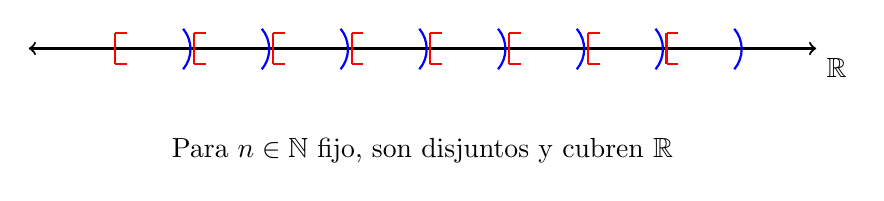
\begin{tikzpicture}
        % Draw the number line
        \draw[thick,<->] (-5,0) -- (5,0) node[anchor=north west] {$\R$};

        % Draw the dyadic intervals of order n=3
        \foreach \j in {-4,...,3} {
            % Draw interval [
            \draw[-, red, thick] (\j+0.1, -0.2) -- (\j+0.1, 0.2);
            \draw[-, red, thick] (\j+0.1, -0.2) -- (\j+0.25, -0.2);
            \draw[-, red, thick] (\j+0.1, 0.2) -- (\j+0.25, 0.2);

            %Draw interval )
            \draw[-, blue, thick] (\j+0.96, 0.25) arc [start angle =40, end angle = -40, radius=0.4];
        }

        % Label the intervals
        \node at (0,-1.3) {Para $n \in \N$ fijo, son disjuntos y cubren $\R$};
    \end{tikzpicture}
\end{center}

\vspace{2mm}
Si $I$ es un intervalo diádico de orden $n$ y $J$ es un intervalo diádico
de orden $m \in \N$ con $m \leq n$: entonces se cumple:
\begin{align*}
    \bullet \hspace{2mm} \text{O bien } I \subsetneq J &&
    \bullet \hspace{2mm} \text{O bien } I \cap J = \varnothing
\end{align*}
La siguiente figura ilustra este hecho:
\vspace{2mm}
\begin{center}
    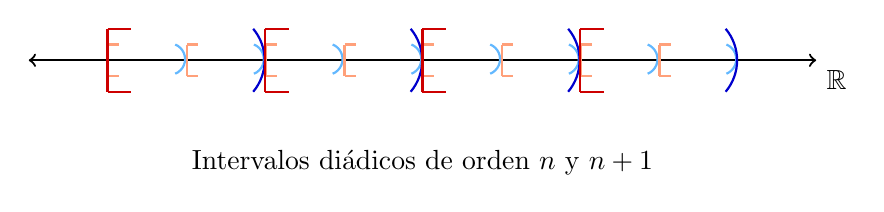
\begin{tikzpicture}
        % Draw the number line
        \draw[thick,<->] (-5,0) -- (5,0) node[anchor=north west] {$\R$};

        % Draw the dyadic intervals of order n=3
        \foreach \j in {-4,...,3} {
            % Draw interval [
            \draw[-, LightSalmon1, thick] (\j+0.01, -0.2) -- (\j+0.01, 0.2);
            \draw[-, LightSalmon1, thick] (\j+0.01, -0.2) -- (\j+0.15, -0.2);
            \draw[-, LightSalmon1, thick] (\j+0.01, 0.2) -- (\j+0.15, 0.2);

            %Draw interval )
            \draw[-, SteelBlue1, thick] (\j+0.86, 0.2) arc [start angle =68, end angle = -68, radius=0.2];
        }

        \foreach \j in {-4, -2, 0, 2} {
            % Draw interval [
            \draw[-, Red3, thick] (\j, -0.4) -- (\j, 0.4);
            \draw[-, Red3, thick] (\j, -0.4) -- (\j+0.3, -0.4);
            \draw[-, Red3, thick] (\j, 0.4) -- (\j+0.3, 0.4);

            %Draw interval )
            \draw[-, Blue3, thick] (\j+1.85, 0.4) arc [start angle =40, end angle = -40, radius=0.6222];
        }
        

        % Label the intervals
        \node at (0,-1.3) {Intervalos diádicos de orden $n$ y $n+1$};
    \end{tikzpicture}
\end{center}

\vspace{6mm}
\result{Definición de cubo diádico}
\hspace{3mm}
Llamamos ``cubo diádico de $\R^N$ de orden $n$'' con $n, N \in \N$ a cualquier conjunto de
la forma $I_1, \times I_2 \times \ldots \times I_N$ donde cada $I_i$ es un intervalo diádico de orden $n$.

\vspace{2mm} \noindent
Denotaremos por $\mathcal{F}_n$ al conjunto de todos los cubos diádicos de orden $n$ en $\R^N$.

\vspace{4mm}
\result{Propiedades de los cubos diádicos}
\hspace{3mm} Los cubos diádicos de orden $n$ son numerables y recubren $R^N$ (consecuencia de la definición y de los resultados anteriores).
Además, son disjuntos o coinciden; es decir:
\begin{align*}
    \left.
    \begin{array}{l}
        C \in \mathcal{F}_n \\
        D \in \mathcal{F}_n \\
        C \neq D
    \end{array}
    \right\}
    \Rightarrow C \cap D = \varnothing
\end{align*}
Como $C,D \in \mathcal{F}_m$, han de ser de la siguiente forma:
\vspace{-2mm}
\begin{align*}
    C = I_1 \times \ldots \times I_N &&
    D = J_1 \times \ldots \times J_N
\end{align*} \\[-5ex]
donde los $I_i$ y los $J_j$ son intervalos diádicos de orden $n$.
Por hipótesis, $C \neq D$ luego ha de existir cierto $k \in \{1, \ldots, n\}$
tal que $I_k \neq J_k$. Por las \hyperref[result:0.2.2]{propiedades de los intervalos diádicos},
sabemos que esto implica que $I_k \cap J_k = \varnothing$. Esto a su vez implica que $C \cap D = \varnothing $.

\vspace{4mm}
De manera similar, si $C \in \mathcal{F}_n, D \in \mathcal{F}_m$ con $m \leq n$. Entonces o bien
$C \subsetneq D$ o bien $C \cap D = \varnothing$. Por definición de $\mathcal{F}_n$ y $\mathcal{F}_m$,
podemos afirmar que:
\begin{align*}
    C = I_1 \times \ldots \times I_N  &&
    D = J_1 \times \ldots \times J_N
\end{align*}
Donde los $I_i$ y los $J_j$ son intervalos diádicos de orden $n$ y $m$, respectivamente. Por las
\hyperref[result:0.2.2]{propiedades de los intervalos diádicos}, para cada $k \in \{1, \ldots, N\}$ se tiene
que o bien $I_k \subsetneq J_k$ o bien $I_k \cap J_k = \varnothing$. Si $\exists k_0 \in \{1, \ldots, N\}$ tal que
$I_{k_0} \cap J_{k_0} = \varnothing$, entonces $C \cap D = \varnothing$. En caso contrario, $C \subsetneq D$.

\vspace{8mm}
\result{Teorema de descomposición de abiertos en cubos diádicos}
\hspace{3mm}
Para todo subconjunto no vacío y abierto en $\left(\R^N, \tau_{R^N}(d)\right)$, $O$, existe una colección numerable
de cubos diádicos (posiblemente de órdenes distintos) de $\R^N$, $\left\{C_n : n \in \N\right\}$, tales que:
\begin{enumerate}[label=\arabic*.)]
    \item $O$ = $\displaystyle \bigcup_{n \in \N} C_n$
    \item $\overline{C_n} \subseteq O \hspace{2mm} \forall n \in \N$
    \item $i \neq j \Rightarrow C_i \cap C_j = \varnothing$
\end{enumerate}

\vspace{4mm}
\dem Definiremos varios conjuntos auxiliares.

\vspace{2mm}
Definimos $\mathcal{G}_n := \left\{C \in \mathcal{F}_n : \overline{C} \subseteq O\right\}$. Cada una de estas colecciones de conjuntos
es finita o numerable al serlo $\mathcal{F}_n$.

\vspace{2mm}
A partir de los $\mathcal{G}_n$ definiremos otra colección de conjuntos.
Para $n = 1$, tomamos $\mathcal{H}_1 := \mathcal{G}_1$.
Para $n >1$, definimos
$$\mathcal{H}_n := \left\{C \in \mathcal{G}_n : C \nsubseteq \displaystyle \bigcup_{k=1}^{n-1}\mathcal{H}_k \right\}
= \left\{C \in \mathcal{G}_n : C \cap \left[\hspace{1mm} \bigcup_{k=1}^{n-1} \hspace{1mm} \bigcup_{D \in \mathcal{H}_k} D_k\right] = \varnothing \right\}$$
La última igualdad se deduce de las \hyperref[result:0.2.4]{propiedades de los cubos diádicos}.
Por construcción, los $\mathcal{H}_n$ son numerables y disjuntos entre sí. Además, por construcción, la clausura de sus cubos
está contenida en $O$. Queda probar el punto (1).

\vspace{2mm}
Intuitivamente, $\mathcal{G}_n$ modela los cubos 
de un cierto orden que ``caben'' en $O$. El paso a los $\mathcal{H}_n$ hace que solo se empiecen a usar cubos ``más pequeños'' en las zonas donde no ``cabrían''
cubos de un orden inferior (``más grandes'').
\\[5ex]
%G_1
\begin{minipage}{0.50\textwidth}
    \begin{center}
    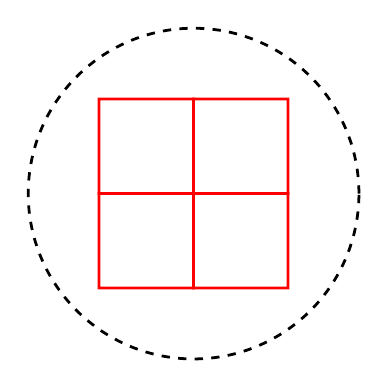
\begin{tikzpicture}[scale=0.6, blend group = normal]
        \draw[-, black, dashed] (0,0) circle (3.5);
        \foreach \i in {-2,0} {
            \foreach \j in {-2,0} {
                \draw[-, red] (\i,\j) rectangle (\i+2, \j+2);
            }
        }
    \end{tikzpicture}
    \\
    $\mathcal{G}_1$
    \end{center}
\end{minipage}
%G_2
\begin{minipage}{0.50\textwidth}
    \begin{center}
        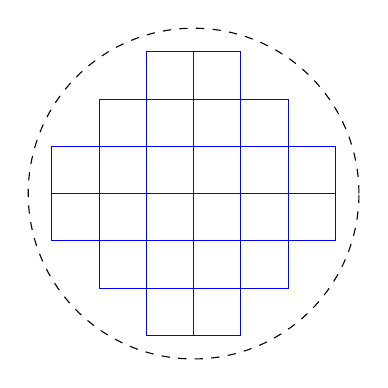
\begin{tikzpicture}[scale=0.6]
            \draw[-, black, dashed] (0,0) circle (3.5);
            \path[draw=blue]
            \foreach \i in {-2,...,1} {
                \foreach \j in {-2,...,1} {
                    (\i,\j) rectangle (\i+1,\j+1)
                }
            }
            \foreach \i in {-1,0} {
                \foreach \j in {-3,2} {
                    (\i,\j) rectangle (\i+1,\j+1)
                    (\j,\i) rectangle (\j+1,\i+1)
                }
            };
        \end{tikzpicture} \\
        $\mathcal{G}_2$
    \end{center}
\end{minipage}
\\[5ex]
%H_1
\begin{minipage}{0.33\textwidth}
    \begin{center}
    \begin{tikzpicture}[scale=0.6]
        \draw[-, black, dashed] (0,0) circle (3.5);
        \foreach \i in {-2,0} {
            \foreach \j in {-2,0} {
                \draw[-, red] (\i,\j) rectangle (\i+2, \j+2);
            }
        }
    \end{tikzpicture}
    $\mathcal{H}_1 = \mathcal{G}_1$
    \end{center}
\end{minipage}
%H_2
\begin{minipage}{0.33\textwidth}
    \begin{center}
        \begin{tikzpicture}[scale=0.6]
            \draw[-, black, dashed] (0,0) circle (3.5);
            \foreach \i in {-1,0} {
                \foreach \j in {-3,2} {
                    \draw[-, blue] (\i,\j) rectangle (\i+1, \j+1);
                    \draw[-, blue] (\j,\i) rectangle (\j+1, \i+1);
                }
            }
        \end{tikzpicture}
        $\mathcal{H}_2$
    \end{center}
\end{minipage}
%H_1 \cup H_2
\begin{minipage}{0.33\textwidth}
    \begin{center}
        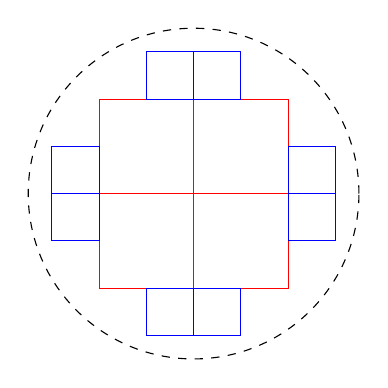
\begin{tikzpicture}[scale=0.6]
            \draw[-, black, dashed] (0,0) circle (3.5);
            \foreach \i in {-2,0} {
                \foreach \j in {-2,0} {
                    \draw[-, red] (\i,\j) rectangle (\i+2, \j+2);
                }        
            }
            \foreach \i in {-1,0} {
                \foreach \j in {-3,2} {
                    \draw[-, blue] (\i,\j) rectangle (\i+1, \j+1);
                    \draw[-, blue] (\j,\i) rectangle (\j+1, \i+1);
                }
            }
        \end{tikzpicture}
        $\mathcal{H}_1 \cup \mathcal{H}_2$
    \end{center}
\end{minipage}
\\[6ex]
Probaremos que \hspace{1mm}
$O = \displaystyle \bigcup_{n \in \N} \hspace{1mm} \bigcup_{C \in \mathcal{H}_n} \hspace{-1mm} C$
\hspace{1mm} por doble contenido.

\begin{tcolorbox}[Subset-contingency]
    $\supseteq$ \hspace{4mm} Por definición de $\mathcal{H}_n$, \hspace{2mm}
    $\forall n \in \N$ se tiene $C \in \mathcal{H}_n \Rightarrow C \subsetneq \overline{C} \subsetneq  O$
\end{tcolorbox}
\begin{tcolorbox}[Subset-contingency]
    $\subseteq $ \hspace{4mm}
    Sea $x_0 \in O \subseteq \R^N$ cualquiera, podemos expresarlo como $x_0 = (x_1, \ldots, x_N)$.
\end{tcolorbox}
Al ser $O$ abierto en $(\R^N, \tau_{\R^N}(d))$, existe $n_0 \in \N$ que verifica:
$$x_0 \in \prod_{i=1}^N \left(x_i - \frac{1}{2^{n_0}},\hspace{1mm}  x_i + \frac{1}{2^{n_0}}\right) \subset \prod_{i=1}^N \left[x_i - \frac{1}{2^{n_0}}, \hspace{1mm} x_i + \frac{1}{2^{n_0}}\right] \subset O$$
Además, para cada coordenada $1 \leq i \leq N$ tenemos que $\exists ! j_i \in \Z : x_i \in \left[\frac{j_i -1}{2^{n_0}}, \frac{j_i}{2^{n_0}} \right)$.
Así, para cada $i \in {1, \ldots, N}$ se tiene que:
\begin{align*}
    \left. \begin{array}{l}
        \frac{j_i - 1}{2^{n_0}} \leq x_i \Rightarrow \frac{j_i}{2^{n_0}} \leq x_i + \frac{1}{2^{n_0}} \\
        x_i < \frac{j_i}{2^{n_0}} \Rightarrow x_i - \frac{1}{2^{n_0}} < \frac{j_i - 1}{2^{n_0}}
    \end{array} \right\} \textstyle
    \Rightarrow \left[\frac{j_i -1}{2^{n_0}}, \frac{j_i}{2^{n_0}} \right) \subset \left(x_i - \frac{1}{2^{n_0}}, x_i + \frac{1}{2^{n_0}} \right)
\end{align*}
De este modo, $D_0 := \displaystyle \prod_{i=1}^{N}\left[\frac{j_i-1}{2^{n_0}}, \frac{j_i}{2^{n_0}} \right) \subsetneq \prod_{i=1}^{N}\left[x_i - \frac{1}{2^{n_0}}, x_i + \frac{1}{2^{n_0}} \right] \subsetneq O$.

\vspace{3mm} \noindent
Y por tanto, $x_0 \in D_0 \subsetneq \overline{D_0} \subsetneq O$. A su vez, como $D_0 \in \mathcal{G}_{n_0}$, hemos demostrado también
que el siguiente conjunto es no vacío: \\[-2.5ex]
$$\mathcal{A}_{x_0} := \Big\{n \in \N : \exists \hspace{1mm} C \in \mathcal{G}_n \text{ tal que } x_0 \in C\Big\} $$

\vspace{4mm}
Al ser $A_{x_0}$ un subconjunto no vacío de $\N$, podemos afirmar que tiene mínimo, al que denotaremos $m_0$. Así, ha de existir $C_0 \in \mathcal{G}_{m_0}$ tal que $x_0 \in C_0$, veamos
que $C_0 \in \mathcal{H}_{m_0}$. Por definición de $\mathcal{H}_{m_0}$, $C_0 \notin \mathcal{H}_{m_0} \Rightarrow C_0 \in \mathcal{G}_n$ para cierto $n < m_0$. Esto contradice
que $m_0$ sea el mínimo de $\mathcal{A}_{x_0}$. Hemos demostrado que $C_0 \in \mathcal{H}_{m_0}$.

\newpage
\chapter{Series dobles}
El álgebra contempla únicamente la suma como operación binaria. Por la propiedad asociativa, es posible expresar cualquier suma finita como sumas binarias sucesivas.
No obstante, el álgebra por sí misma no nos basta para sumar series.

\vspace{4mm}
\result{Definición de sucesión doble}
\hspace{3mm} Llamamos ``sucesión doble'' a cualquier aplicación
\begin{flalign*}
    \hspace{2mm} \gamma : \N \times \N &\longrightarrow \overline{\R} = \R \cup \{+\infty -\infty\} &&\\
    \hspace{2mm} n, m &\longmapsto \gamma(n,m) = a_{nm} &&
\end{flalign*} \\[-5ex]
Diremos que $a_{nm}$ es el término general de la sucesión.

\vspace{4mm}
\result{Definición de serie doble}
\hspace{3mm} Dada una sucesión doble de término general $a_{nm}$, llamamos ``serie doble de término general $a_{nm}$''
a la expresión $\displaystyle \sum_{n,m} a_{nm}$ (que equivale a $\displaystyle \sum_{\substack{n = 1\\m=1}}a_{nm}$ \hspace{2mm}).

\vspace{4mm}
Diremos que $\sum_{n,m}a_{nm}$ es convergente si sus sumas parciales convergen a un número real. Es decir, si:
$\exists s \in \R $ que verifica: \\[-4ex]
$$ \forall\hspace{1mm}\varepsilon > 0 \hspace{2mm} \exists \hspace{1mm} n_0 \in \N \text{ tal que }\hspace{2mm}  n,m \geq n_0 \Rightarrow
\left|s - \sum_{\substack{1\leq i \leq n\\1\leq j \leq m}}a_{ij}\right| < \varepsilon$$
En este caso, diremos que este $s$ es el ``valor de la suma de la serie''.

\vspace{4mm}
Diremos que $\sum_{n,m} a_{nm}$ es divergente a $+\infty (-\infty)$ si $\forall K\hspace{1mm} \in \R$
$\exists \hspace{1mm} n_0  \in \N$ tal que dados $n, m \geq n_0$ se cumple: \\[-5ex]
\begin{align*}
    \sum_{\substack{1\leq i \leq n\\1 \leq j \leq m}}a_{ij} > K &&
    \left(\sum_{\substack{1\leq i \leq n\\1 \leq j \leq m}}a_{ij} < K\right)
\end{align*}
En este caso, diremos que el valor de la suma de la sucesión es $+\infty (-\infty)$.

Es importante distinguir la igualdad de series como sucesiones y como valores. Veamos un ejemplo
con series simples: \\[-5ex]
\begin{align*}
    \sum_{n=1}^\infty a_n = 1 +0+0+0+\ldots &&
    \sum_{n=1}^\infty b_n = \frac{1}{2} + \frac{1}{4} + \frac{1}{8} + \frac{1}{16} + \ldots
\end{align*} \\[-4ex]
Es claro que las series no tienen el mismo término general (no son iguales como series), pero sí tienen el mismo valor de suma (que es 1).

\vspace{6mm}
\result{Teorema de series dobles no negativas}
\hspace{3mm} Dada una sucesión doble $\gamma : \N \times \N \longrightarrow [0, +\infty]$ de término general $a_{nm}$,
dada una biyección cualquiera $g : \N \longrightarrow \N \times \N$, se cumple:
\begin{align*}
    \sum_{n,m} a_{nm} = \sum_{n = 1}^{\infty}a_{g(n)} = \sum_{n=1}^{\infty}\sum_{m=1}^{\infty}a_{nm} = \sum_{m=1}^{\infty}\sum_{n=1}^{\infty}a_{nm} \in[0, +\infty]
\end{align*}
\dem Probaremos primero la igualdad respecto de la reordenación y después respecto de las series anidadas.

\vspace{2mm}
Si existe algún término $a_{n_0m_0} = +\infty$, entonces la igualdad se cumple trivialmente al estar las sumas bien definidas ($\gamma(\N \times \N) \subseteq[0, +\infty])$.
Supongamos entonces que todos los términos son finitos, veamos qué casos pueden darse:

\vspace{5mm}
$\bullet$ Primer caso: Supongamos que $\displaystyle{\sum_{n=1}^{\infty}a_{g(n)}} = s \in \R$.

\noindent
Por definición, $\forall \varepsilon > 0 \hspace{1mm} \exists \hspace{1mm} n_0 \in \N : \hspace{2mm} s - \displaystyle{\sum_{k=1}^{n}a_{g(k)}} < \varepsilon \hspace{2mm} \forall n \geq n_0$.
Sea $\varepsilon > 0$ cualquiera pero fijo, fijamos también el $n_0$ asociado.
Como $g$ es biyectiva, $\exists \hspace{1mm} m_0 \in \N$ tal que $g(\{1,\ldots,n_0\}) \subseteq \{1,\ldots, m_0\} \times \{1,\ldots,m_0\}$.
Al tratarse de series de términos no negativos, dados $n,m \in \N$ con $n\geq n_0, m\geq n_0$, se cumple:
$$\sum_{k=1}^{n_0}a_{g(k)} \leq \sum_{\substack{1\leq i \leq n\\1\leq j \leq m}}a_{ij}
\Rightarrow 0 \overset{(*)}{\leq} s -  \sum_{\substack{1\leq i \leq n\\1\leq j \leq m}}a_{ij} \leq s - \sum_{k=1}^{n_0}a_{g(k)} < \varepsilon$$
(*) La desigualdad se deduce de que la suma parcial de la serie doble es una reordenación de la suma parcial de la serie simple, siendo esta última absolutamente convergente.
Como podemos hacer $\varepsilon$ arbitrariamente pequeño, concluimos que las dos series tienen el mismo límite.

\vspace{4mm}
$\bullet$ Segundo caso: $\smallsum_{n=1}^\infty a_{g(n)} = +\infty$.

\vspace{2mm}
Sea $K \in \R$, por definición, $\exists \hspace{1mm} n_0 \in \N \text{ tal que } \smallsum_{k=1}^{n} a_{g(k)} > K \hspace{2mm} \forall \hspace{1mm} n \geq n_0$.
Al ser $g$ biyectiva, $\exists \hspace{1mm} m_0 \in \N \text{ tal que } g({1,\ldots,n_0}) \subseteq \{1,\ldots, m_0\} \times \{1,\ldots,m_0\}$. Así, dados $n \geq m_0, m\geq m_0$ se tiene:
\\[-3ex] $$K < \sum_{k=1}^{n_0} a_{g(k)} \leq \sum_{\substack{1\leq i \leq n\\1\leq j \leq m}} a_{ij}$$
Es claro que la serie doble diverge a $+\infty$.

\vspace{4mm}
Queda probar la igualdad entre la serie doble y las series anidadas cuando todos los términos son finitos. Veamos qué ocurre según el carácter de la serie doble.

\vspace{4mm}
$\bullet$ Primer caso: $\sum_{n,m}a_{nm} = s \in [0,+\infty)$.

\vspace{2mm}
Sea $\varepsilon > 0$. Por definición de convergencia, sabemos que
$\exists \hspace{1mm} n_0 \in \N \text{ tal que dados } n\geq n_0, m\geq n_0$ se tiene:
$$\left|\hspace{1mm} s - \sum_{\substack{1\leq i \leq n\\1\leq j \leq m}} a_{ij} \hspace{1mm} \right| < \varepsilon$$
\\[1mm]
Nótese que debido a las propiedades algebraicas de la suma, en el caso finito se da la igualdad; es decir:
\\[-3.5ex]
$$\sum_{\substack{1\leq i \leq n\\1\leq j \leq m}} a_{ij} = \sum_{i=1}^n\sum_{j=1}^m a_{ij} = \sum_{j=1}^m\sum_{i=1}^n a_{ij}$$
De este modo, sustituyendo en la definición de convergencia, dados $n \geq n_0, m\geq n_0$ obtenemos:
\begin{flalign*}
    \left|\hspace{1mm}s- \sum_{j=1}^m\sum_{i=1}^n a_{ij} \hspace{1mm}\right| < \varepsilon
    \Rightarrow \varepsilon \geq \lim_n \left|\hspace{1mm} s - \sum_{j=1}^m\sum_{i=1}^n a_{ij} \hspace{1mm}\right|
    = \left|\hspace{1mm} s - \sum_{j=1}^m \lim_n \left( \sum_{i=1}^n a_{ij} \right)\hspace{1mm}\right|
\end{flalign*}
La igualdad se debe a aplicar las propiedades del límite con funciones continuas. Como la serie doble converge por hipótesis,
también han de hacerlo las series de filas y columnas. Es por ello que podemos afirmar que el último límite existe.

\vspace{2mm}
La igualdad anterior se cumple para cualquier $\varepsilon > 0$ y para cualquier $m \geq n_0$. Haciendo $\varepsilon$
arbitrariamente pequeño y tomando límites en $m$ llegamos al resultado. El razonamiento para la otra serie anidada es análogo; así, concluimos:
\begin{flalign*}
    \sum_{m=1}^\infty\sum_{n=1}^\infty a_{nm} = \sum_{n=1}^{\infty}\sum_{m=1}^{\infty}a_{nm} = \sum_{n,m}a_{nm}
\end{flalign*}

\vspace{4mm}
$\bullet$ Segundo caso: $\sum_{n,m}a_{nm} = +\infty$. Si hubiese algún $n\in \N$ verificando $\sum_{m=1}^\infty a_{nm} = +\infty$ 
o si existiese algún $m \in \N$ tal que $\sum_{n=1}^{\infty}a_{nm} = +\infty$, las series anidadas divergerían trivialmente.
Supongamos que no es el caso para ver que también se cumple el resultado.

\vspace{2mm}
Sea $K \in \R$ cualquiera, por definición de divergencia se cumple:
\begin{flalign*}
    \exists \hspace{1mm} n_0 \in \N \text{ tal que } \forall \hspace{1mm} n \geq n_0, \forall m \geq n_0 \text{ se cumple } \sum_{j=1}^{m}\sum_{i=1}^n a_{ij} > K
\end{flalign*}
Nótese que hemos utilizado la igualdad entre la serie doble y las series anidadas para el caso finito. Además, dados $n \geq n_0, m \geq n_0$, se cumple:
\begin{flalign*}
    \sum_{j=1}^{m}\sum_{i=1}^{n} a_{ij} > K
    \Rightarrow K \leq \lim_n \sum_{j=1}^{m}\sum_{i=1}^{n} a_{ij}
    = \sum_{j=1}^{m} \left( \sum_{i=1}^{\infty} a_{ij}\right)
\end{flalign*}
Las series de suma de filas y columnas existen por hipótesis, luego la igualdad se cumple para todo $m \geq n_0$. Tomando límites en $m$ podemos observar que
$\sum_{m=1}^\infty \sum_{n=1}^\infty a_{nm} \geq K$. Como el $K$ escogido fue arbitrario, se cumple para cualquier $K$ real.
Así, las series anidadas divergen a $+\infty$ (análogo para la otra serie anidada).

\newpage
\unit{Teoría de la medida}

\vspace{2mm}
\chapter{Espacios de medida}
\result{Definición de \texorpdfstring{$\sigma$}{s}-álgebra}
\hspace{3mm} Sea $X$ un conjunto cualquiera, diremos que $\Sigma \subseteq \mathcal{P}(X)$ es una $\sigma$-álgebra si cumple las siguientes propiedades:
\begin{enumerate}[label=S.\arabic*)]
    \item $\varnothing \in \Sigma$
    \item $\left\{E_i : i\in \N\right\} \subseteq \Sigma \Rightarrow \displaystyle{\bigcup_{i \in \N}{E_i}} \in \Sigma$
    \item $E \in \Sigma \Rightarrow E^c := X \backslash E \in \Sigma$
\end{enumerate}
Nótese que no es necesario exigir que $X$ tenga ningún tipo de estructura (ni topológica, ni algebraica...).

\vspace{4mm}
\result{Propiedades de las \texorpdfstring{$\sigma$}{s}-álgebras}
\hspace{3mm} Sea $X$ un conjunto, sea $\Sigma$ una $\sigma$-álgebra de $X$.
Sea $\{E_i : i \in \N\} \subseteq \Sigma$, y $E,F \in \Sigma$. Entonces, se cumple:
\begin{enumerate}[label=\roman*)]
    \item $\displaystyle{\bigcap_{i\in\N}{E_i}} \in \Sigma$
    \item $E\cup F \in \Sigma$
    \item $E \cap F \in \Sigma$
    \item $E \backslash F \in \Sigma$
\end{enumerate}

\vspace{2mm} \dem

\vspace{2mm}
$\romannumeral 1)$ Por la propiedad $(S.3)$ y la involución del complementario, un conjunto pertenece a una $\sigma$-álgebra si y solo si su complementario pertenece a ella.
Por tanto, basta ver que: \hspace{2mm}
$X \setminus \left(\bigcap_{i\in\N}{E_i}\right)
= \displaystyle{\bigcup_{i\in\N}{\left(X \setminus E_i\right)}} \in \Sigma$.

Por la propiedad $(S.3)$, para cada $i \in \N$ tenemos que $X\setminus E_i \in \Sigma$, pues $E_i \in \Sigma$ por hipótesis.
Finalmente, aplicando $(S.1)$ tenemos que su unión numerable se encuentra en $\Sigma$.

\vspace{4mm}
$\romannumeral 2)$ Reescribiremos $E\cup F$ para hacer uso del resultado que acabamos de probar.
Por $(S.1)$ sabemos que $\varnothing \in \Sigma$ luego podemos considerar la colección numerable de conjuntos de $\Sigma$,
$\{A_i : i \in \N\}$ donde $A_1 = E, \hspace{2mm} A_2 = F$, y $ A_n = \varnothing  \hspace{2mm} \forall \hspace{1mm} n > 2$.

\vspace{2mm} \noindent
De este modo, $E \cup F = E \cup F \cup \varnothing  \cup \varnothing \cup \ldots = \displaystyle{\bigcup_{i \in \N}{A_i}} \in \Sigma$.

\vspace{4mm}
$\romannumeral 3)$ Como consecuencia de $(S.1)$ y de $(S.3)$, sabemos que $X \in \Sigma$.
Así, basta considerar $B_1 = E,$ $B_2 = F$, $B_n = X \hspace{2mm} \forall \hspace{1mm} n > 2$.

\vspace{2mm} \noindent
Aplicando el apartado $(\romannumeral 1)$, $E \cap F = E \cap F \cap X \cap X \cap \ldots
= \displaystyle{\bigcap_{i \in \N}{B_i}} \in \Sigma$.

\vspace{4mm}
$\romannumeral 4)$ Por definición de complementario, $E\setminus F = E \cap (X \setminus F)$.
Por hipótesis, $E,F\in \Sigma$. Aplicando $(S.3)$, $(X\setminus F)\in \Sigma$.
Finalmente, aplicando el apartado $(\romannumeral 3)$, $E \cap (X \setminus F) \in \Sigma$.

\vspace{6mm}
\result{Definición de espacio de medida}
\hspace{3mm} Sea $X$ un conjunto cualquiera y $\Sigma$ una $\sigma$-álgebra de $X$, diremos que \newline
$\mu : \Sigma \longrightarrow [0,+\infty]$ es una medida sobre $\Sigma$ si verifica las siguientes propiedades:
\begin{enumerate}[label=M.\arabic*)]
    \item $\mu(\varnothing) = 0$
    \item Sean $\{E_i : i\in \N\} \subseteq \Sigma$ tales que $i \neq j \Rightarrow E_i \cap E_j = \varnothing $; entonces,
    $$\mu\left(\bigcup_{i\in \N} E_i\right) = \sum_{i\in \N} \mu(E_i)$$
\end{enumerate}

\vspace{2mm}
A la tríada $(X, \Sigma, \mu)$ se la denomina ``espacio de medida'', y a los conjuntos
de $\Sigma$ se los llama ``conjuntos ($\mu$-)medibles de $X$''.

\result{Propiedades de los espacios de medida}
\hspace{3mm} Sea $(X,\Sigma,\mu)$ un espacio de medida, se cumple:
\begin{enumerate}[label=\roman*)]
    \item Sean $E,F\in \Sigma$ con $F \subseteq E$, se cumple $\mu(F) \leq \mu(E)$.
    \newline \noindent
    Si además se tiene que $\mu(F) < +\infty$, entonces $\mu(E \setminus F) = \mu(E) - \mu(F)$.
    
    \item Sean $\{E_i : i \in \N\} \subseteq \Sigma$ tales que $E_i \subseteq E_{i+1} \hspace{2mm}\forall \hspace{1mm} i \in \N$.
    \newline\noindent
    Entonces, $\mu (\smallcup_{i \in \N}{E_i}) = \displaystyle{\lim_n \mu(E_n)}$.
    
    \item Sean $\{E_i : i \in \N\} \subseteq \Sigma$ tales que $E_{i+1} \subseteq E_{i} \hspace{2mm}\forall \hspace{1mm} i \in \N$, y $\mu(E_1) < +\infty$.
    \newline \noindent
    Entonces, $\mu(\smallcap_{i\in\N}E_i) = \mlim{n} \hspace{1mm} \mu(E_n)$.
\end{enumerate}

\vspace{2mm} \dem

\vspace{2mm}
$\romannumeral 1)$ Reescribiendo como unión numerable
de conjuntos disjuntos de $\Sigma$, \\[-5ex]
\begin{flalign*}
    E = (E \setminus F) \cup F \cup \varnothing \cup \varnothing \cup\ldots 
\end{flalign*}
\\[-5ex]
Aplicando $(M.3)$ y evaluando $\mu$ a ambos lados obtenemos:
\\[-5ex]
\begin{flalign*}
    \mu(E) = \mu(E \setminus F) + \mu(F) + \mu(\varnothing) + \mu(\varnothing) + \ldots    
\end{flalign*}
Aplicando $(M.1)$ se deduce que $\mu(E) = \mu(E \setminus F) + \mu(F)$.
Por la no negatividad de $\mu$, se tiene que $\hspace{1mm} \mu(E \setminus F) \geq 0 \Rightarrow \mu(F) \leq \mu(F)$.

\vspace{2mm} \noindent
Si además $\mu(F) < +\infty$, podemos despejar sin que ocurran indeterminaciones; así, $\mu(E \setminus F) = \mu(E) - \mu(F)$.

\vspace{8mm}
$\romannumeral 2)$ Una vez más, reescribimos el conjunto a partir de uniones disjuntas:
$$\bigcup_{i\in \N} E_i = E_1 \cup \Big(E_2 \setminus E_1\Big) \cup \Big(E_3 \setminus (E_2 \cup E_1)\Big)
\cup \Big(E_4 \setminus (E_1 \cup E_2 \cup E_3)\Big) \cup \ldots$$
Como $E_i \subseteq E_{i+1}$ por hipótesis, podemos simplificar esta expresión: \\[-3ex]
$$\bigcup_{i\in \N}E_i = E_1 \cup (E_2 \setminus E_1) \cup (E_3 \setminus E_2)
\cup (E_4 \setminus E_3)\cup \ldots = E_1 \cup \left(\bigcup_{i \in \N}(E_{i+1}\setminus E_i)\right)$$
Así, $\hspace{2mm} \displaystyle \mu\left(\bigcup_{i\in\N}E_i\right)= \mu(E_1) + \sum_{i=2}^{\infty}\mu(E_{i}\setminus E_{i-1}) = (*)$.

\noindent
Distinguimos dos casos en función de la medida de los $E_i$:

\vspace{2mm}
$\romannumeral 2.a)$ Existe cierto $j \in \N$ tal que $\mu(E_j) = +\infty$.
Como $E_j \subseteq E_n \hspace{2mm} \forall \hspace{1mm} n \geq j$, aplicando \hyperref[result:1.1.4]{las propiedad $(i)$ de la medida},
se tiene que $\mu(E_n) = +\infty \hspace{2mm} \forall \hspace{1mm} n \geq j$,
luego ha de cumplirse $\mlim{n} \hspace{1mm}\mu(E_n) = +\infty$.
Por otro lado, como $E_j \subseteq \smallcup_{i\in \N} E_i$, se tiene que
$+\infty = \mu(E_j) \leq \mu(\smallcup_{i\in\N}E_i)$,
luego, $\mlim{n} \hspace{1mm} \mu(E_n) = \mu(\smallcup_{i\in\N}E_i) = +\infty$.

\vspace{4mm}
$\romannumeral 2.b)$ En caso contrario al anterior, $\mu(E_i) < +\infty \hspace{2mm} \forall \hspace{1mm} i \in \N$. Desarrollando en $(*)$,
\begin{flalign*}
    \mu\Big(\smallcup_{i\in\N} &E_i\Big) = \mu(E_1) + \sum_{i=2}^{\infty}\mu(E_{i}\setminus E_{i-1})
    = \mu(1) + \lim_n \sum_{i=2}^{n}\mu(E_i \setminus E_{i-1}) = \\
    &= \lim_n \Big(\mu(E_1) + \mu(E_2 \setminus E_1) + \mu(E_3 \setminus E_2) + \ldots + \mu(E_{n} \setminus E_{n-1}) \Big) = \\
    &= \lim_n \Big(\mu(E_1) + \big(\mu(E_2) - \mu(E_1)\big) + \ldots + \big(\mu(E_n) - \mu(E_{n-1})\big)\Big) = \\
    &= \lim_n \mu(E_n)
\end{flalign*}
Hemos podido simplificar porque todas las medidas son finitas; de lo contrario, podrían producirse indeterminaciones.

\vspace{8mm}
$\romannumeral 3)$ Por hipótesis, $E_{i+1} \subseteq E_i \hspace{2mm} \forall \hspace{1mm} i \in \N$, y $\mu(E_1) < +\infty$.
De este modo, como todos los $E_i$ son subconjuntos de $E_1$ han de tener medida finita también (\hyperref[result:1.1.4]{propiedad $(i)$ de la medida}).
Expresamos la intersección según el complementario respecto de $E_1$ como sigue:
$\hspace{2mm} E_1 \setminus \big(\smallcap_{i\in\N}E_i\big) = \smallcup_{i\in\N}\big(E_1 \setminus E_i\big)$.

\vspace{4mm} \noindent
Por hipótesis, $E_{i+1} \subseteq E_i \Rightarrow (E_1 \setminus E_i) \subseteq (E_1\setminus E_{i+1})$.
Como consecuencia, aplicando los apartados anteriores de este resultado,
\begin{flalign*}
    \mu(E_1) - \mu\Big(\smallcap_{i\in\N}E_i\Big)
    &=\mu\Big(E_1 \setminus\big(\smallcap_{i\in\N}E_i\big)\Big)
    = \mu\Big(\smallcup_{i\in\N}(E_1 \setminus E_i)\Big) =\\[1ex]
    &= \lim_n \mu(E_1 \setminus E_n)
    = \mu(E_1) - \lim_n \mu(E_n)
\end{flalign*}
Como todas las medidas son finitas, podemos despejar sin indeterminaciones: 
$$\mu\Big(\smallcap_{i\in\N}E_i\Big) = \lim_n \mu(E_n)$$

\result{Espacio de medida inducido}
\hspace{3mm} Dado un espacio de medida $(X, \Sigma, \mu)$. Sea $A \in \Sigma$ cualquiera,
definimos la siguiente colección $\Sigma(A) := \{B\cap A : B \in \Sigma\}$. Entonces, $(A, \Sigma(A), \mu_{|\Sigma(A)})$ es un espacio de medida.

\vspace{4mm}
\dem Comencemos comprobando que $\Sigma(A)$ es en efecto una $\sigma$-álgebra.

\vspace{2mm}
$(S.1)$ Por ser $\Sigma$ una $\sigma$-álgebra, $\varnothing \in \Sigma$.
Así, basta tomar $B = \varnothing$. De este modo, $\varnothing = A \cap \varnothing \in \Sigma(A)$.

\vspace{4mm}
$(S.2)$ Sean $\{E_i : i \in \N\} \subseteq \Sigma(A)$, buscamos $\smallcup_{i \in \N} E_i \in \Sigma(A)$.
Por definición de $\Sigma(A)$, cada $E_i$ será de la forma $A\cap F_i$ con $F_i \in \Sigma$. Así, se tiene:
\\[-4ex]\begin{flalign*}
    \bigcup_{i\in\N}E_i = \bigcup_{i\in\N}A\cap F_i = A\cap \left(\bigcup_{i\in\N}F_i\right) \in \Sigma(A)
\end{flalign*} \\[-4ex]
Consideramos $B = \smallcup_{i\in\N}F_i \in \Sigma$ al aplicar $(S.2)$ en $\Sigma$.

\vspace{6mm}
$(S.3)$ Sea $E \in \Sigma(A)$, buscamos $A \setminus E \in \Sigma(A)$. Por definición de $\Sigma(A)$,
podemos afirmar que $E = A \cap B$ para cierto $B \in \Sigma$. Aplicando $(S.3)$, por ser $\Sigma$ una
$\sigma$-álgebra de $X$, $B \in \Sigma \Rightarrow X \setminus B \in \Sigma$.
Así, $A \setminus E = A \cap (X \setminus B) \in \Sigma(A)$.

\vspace{4mm} \noindent
Queda ver que $\mu_{|\Sigma(A)}$ es una medida. Como $\Sigma(A) \subseteq \Sigma$, las propiedades de $\mu$ se trasladan
trivialmente a $\mu_{|\Sigma(A)}$.

\vspace{4mm}
\nota Para definir una $\sigma$-álgebra inducida basta tomar $A \subseteq X$ cualquiera.
No obstante, para que $\mu_{|\Sigma(A)}$ sea una medida, necesitamos que $\Sigma(A) \subseteq \Sigma$, y
para ello es necesario exigir $A \in \Sigma$.

\newpage
\result{Medida de contar}
Veamos dos ejemplos de espacios de medida:

\vspace{4mm}
$\bullet (\N, \mathcal{P}(\N), m)$ donde $m$ es la ``medida de contar'' y se define como
\begin{flalign*}
    m(A) = \begin{cases}
        \card A &\text{ si } A \text{ es finito}\\
        +\infty &\text{ en otro caso}
    \end{cases}
\end{flalign*}

\vspace{2mm}
$\bullet (\R, \mathcal{P}(\R), \mu)$ donde $\mu(B) = m(B \cap\N)$.

\vspace{4mm}
Al ser el conjunto de partes una $\sigma$-álgebra trivialmente, basta ver que las medidas cumplen $(M.1)$ y $(M.2)$,
lo que es evidente en vista de su definición.

\vspace{4mm}
En este tema buscamos establecer una medida en $\R^N$ basada en la longitud de los intervalos. Hemos de definir
adecuadamente la $\sigma$-álgebra asociada, pues ha de incluir a todos los intervalos (y por tanto a todos los abiertos) y 
a sus complementarios (luego todos los cerrados). Sin embargo, como veremos más adelante, no es posible tomar simplemente $\mathcal{P}(\R^N)$.

\vspace{6mm}
\result{Subaditividad en espacios de medida}
\hspace{3mm} Sea $(X, \Sigma, \mu)$ un espacio de medida, sean $\{E_i : i \in \N\} \subseteq \Sigma$.
Entonces, se cumple: \\[-3ex]
$$\mu(\smallcup_{i \in \N} E_i) \leq \smallsum_{i \in\N}\mu(E_i)$$

\vspace{4mm}
\dem Expresaremos $\smallcup_{i\in\N}E_i$ como unión de conjuntos disjuntos.

\vspace{4mm}
Definimos $F_1 := E_1 \in \Sigma$. Para todo $n \in \N$, $E_1 \cup E_2 \cup \ldots \cup E_n \in \Sigma$.
Así, $F_{n+1} := E_{n+1} \setminus (E_1 \cup \ldots \cup E_n) \in \Sigma$.
Veamos que $\smallcup_{i\in\N}F_i = \smallcup_{i\in\N}E_i$ por doble contenido.

\vspace{4mm}
\begin{tcolorbox}[Subset-contingency]
    $\subseteq$ \hspace{3mm} $\forall \hspace{1mm} i \in \N$, $F_i \subseteq E_i \Rightarrow \smallcup_{i\in\N}F_i \subseteq \smallcup_{i\in\N}E_i$.
\end{tcolorbox}
\begin{tcolorbox}[Subset-contingency]
    $\supseteq$ \hspace{3mm} Sea $x_0 \in \smallcup_{i\in\N} E_i$; por definición, $\exists \hspace{1mm} i_0 \in \N$ tal que $x_0 \in E_{i_0}$.
\end{tcolorbox}
Por tanto, el siguiente conjunto $\mathcal{A}_{x_0}$ es no vacío:
$ \mathcal{A}_{x_0} := \left\{n \in \N : x_0 \in E_n\right\}$.
Al ser un subconjunto no vacío de $\N$, podemos afirmar que existe $m_0 := \min \mathcal{A}_{x_0}$.
Por definición de $\mathcal{A}_{x_0}$
\begin{flalign*}
    \left. \begin{array}{l}
        x_0 \in E_{m_0} \\
        x_0 \notin E_i \hspace{2mm} \forall \hspace{1mm} i < m_0
    \end{array} \right\}
    \Rightarrow x_0 \in F_{m_0} \subseteq \smallcup_{i\in\N} F_i
\end{flalign*}
\vspace{2mm}
Volviendo al problema de la subaditividad, se cumple: \\[-6ex]
\begin{flalign*}
    \mu(\smallcup_{i\in\N}E_i) = \mu(\smallcup_{i\in\N}F_i) = \mu(F_1) + \mu(F_2) + \ldots
    \leq \mu(E_1) + \mu(E_2) + \ldots = \smallsum_{i\in\N} \mu(E_i)
\end{flalign*} \\[-4ex]
La desigualdad se debe a que $\forall \hspace{1mm} i \in \N, F_i \subseteq F_i \Rightarrow \mu(F_i) \leq \mu(E_i)$.

\vspace{6mm}
\result{Definición de espacio de medida completo}
\hspace{3mm} Sea $(X, \Sigma, \mu)$ un espacio de medida, diremos que es un ``completo''
(o que $\Sigma$ es completo respecto de $\mu$) si se cumple: \\[-4ex]
\begin{flalign*}
    \forall \hspace{1mm} B \in \Sigma \text{ con } \mu(B) = 0,
    \hspace{2mm} \forall \hspace{1mm} A \subseteq B \text{ se tiene que } A \in \Sigma
    \text{ y por tanto } \mu(A) = 0
\end{flalign*}

\vspace{6mm}
\result{Compleción de un espacio de medida}
\hspace{3mm} Sea $(X, \Sigma, \mu)$ un espacio de medida cualquiera. Existe una $\sigma$-álgebra $\tilde{\Sigma}$ de $X$ con $\Sigma \subseteq \tilde{\Sigma}$.
y una medida $\tilde{\mu}$ sobre $\tilde{\Sigma}$ tales que $\tilde{\mu}_{|\Sigma} = \mu$
\hspace{1mm} y \hspace{1mm} $(X, \tilde{\Sigma},\tilde{\mu})$ es completo.

\vspace{2mm}
De hecho, podemos hallar $\tilde{\Sigma}$ y $\tilde{\mu}$ para que $(X, \tilde{\Sigma}, \tilde{\mu})$ sea el
menor espacio completo que contiene a $(X, \Sigma, \mu)$. Es decir, sea $(X, \Omega, \nu)$ un espacio de medida completo
tal que $\Sigma \subseteq \Omega$ \hspace{1mm} y \hspace{1mm} $\nu_{|\Sigma} = \mu$; entonces, $\tilde{\Sigma} \subseteq \Omega$.

\vspace{2mm} \noindent
En tal caso, diremos que $(X, \tilde{\Sigma}, \tilde{\mu})$ es la ``compleción de $(X, \Sigma, \mu)$''.

\newpage
\dem Definiremos el siguiente conjunto auxiliar: \\[-3ex]
$$\mathcal{N} := \{N \in \mathcal{P}(X) : \exists \hspace{1mm} B \in \Sigma \text{ tal que } N \subseteq B \text{ y } \mu(B) = 0\} $$
\\[-4ex]
Intuitivamente, $\mathcal{N}$ contiene todos los conjuntos que podrían faltarle a $\Sigma$ para que $(X, \Sigma, \mu)$ fuese un espacio de medida completo.
Veamos cómo expandir $\Sigma$ incluyendo estos conjuntos sin introducir otros nuevos que necesitemos completar.

\vspace{2mm} \noindent
Basta considerar la siguiente definición de $\tilde{\Sigma}$: \\[-2.5ex]
$$\tilde{\Sigma} := \{A \cup N : A \in \Sigma, N \in \mathcal{N}\}$$

Para verificar que $\tilde{\Sigma}$ cumple las propiedades que deseamos, introduciremos la siguiente observación:
Sean $A \in \Sigma, N \in \mathcal{N}$. Existen $N_0 \in \mathcal{N}$, $M \in \Sigma$ tales que:
\\[-5ex]
\begin{flalign*}
    A \cup N = A \cup N_0 &&
    N_0 \subseteq M &&
    \mu(M) = 0 &&
    A \cap M = \varnothing
\end{flalign*}
\\[-6ex]
Veamos la demostración:
%Observación dentro de una demostración mayor
\begin{adjustwidth}{0.10\textwidth}{}
    Al considerar $N_0 := N \setminus A$ es claro que $A \cup N = A \cup (N \setminus A) = A \cup N_0$.
    \newline
    Como $N\in \mathcal{N}$, se tiene que $\exists \hspace{1mm} B \in \Sigma$ con $N \subseteq B$ y $\mu(B) = 0$. 
    \newline
    Así, tomando $M := B \setminus A \in \Sigma$ se cumple $A \cap M = \varnothing$.
    \newline
    Además, $N \subseteq B \Rightarrow N_0 = N \setminus A \subseteq B \setminus A = M$.
    \newline
    Finalmente, $M \subseteq B \Rightarrow 0 \leq \mu(M) \leq \mu(B) = 0 \Rightarrow \mu(M) = 0$.
\end{adjustwidth}
\vspace{4mm}
Comprobemos ahora que $\tilde{\Sigma}$ es en efecto una $\sigma$-álgebra de $X$.

\vspace{4mm} \noindent
$(S.1)$ Buscamos $\varnothing \in \tilde{\Sigma}$
\begin{adjustwidth}{0.10\textwidth}{}
    Para ello hay que expresar $\varnothing = A \cup N$ con $A \in \Sigma$, $N \in \mathcal{N}$.
    \newline \noindent
    Tenemos que $\varnothing \in \Sigma$ por ser $\Sigma$ una $\sigma$-álgebra.
    \newline \noindent
    Además, $\varnothing \subseteq \varnothing$ con $\varnothing \in \Sigma$ y $\mu(\varnothing) = 0$.
    \newline \noindent
    Por tanto, tenemos que $\varnothing \in \mathcal{N}$ al tomar $B = \varnothing$ en la definición de $\mathcal{N}$.
    \newline \noindent
    Así, tomando $A = N = \varnothing$, \hspace{1mm}$\varnothing = A \cup N= \varnothing \cup \varnothing \in \tilde{\Sigma}$.
\end{adjustwidth}
\vspace{4mm}\noindent
$(S.2)$ Sean $\{E_i : i \in \N\} \subseteq \tilde{\Sigma}$, buscamos $\smallcup_{i\in\N}E_i \in \tilde{\Sigma}$.
\begin{adjustwidth}{0.1\textwidth}{}
    Por definición de $\tilde{\Sigma}$, $\forall \hspace{1mm} j \in \N :$ $E_j = A_j \cup N_j$ con $A_j \in \Sigma$, $N_j \in \mathcal{N}$.
    \vspace{2mm}\newline\noindent
    Entonces, \hspace{1mm} $\smallcup_{i \in \N}E_i = \smallcup_{i\in\N}(A_i \cup N_i) = \big(\smallcup_{i\in\N}A_i\big)\cup\big(\smallcup_{i\in\N}N_i\big)$.
    \vspace{3mm} \newline \noindent
    Se tiene $\smallcup_{i\in\N}A_i \in \Sigma$. Queda ver $\smallcup_{i\in\N}N_i \in \mathcal{N}$ para llegar al resultado.
    \newpage \noindent
    Por definición de $\mathcal{N}$, $\forall \hspace{1mm} j \in \N :$  $\exists \hspace{1mm} B_j \in \Sigma$ con $N_j \subseteq B_j$ y $\mu(B_j) = 0$.
    \vspace{3mm} \newline \noindent
    Así, $\smallcup_{i\in\N}N_i \subseteq \smallcup_{i\in\N}M_i$ y $0 \leq \mu(\smallcup_{i\in\N}B_i) \leq \smallsum_{i\in\N}\mu(B_i) = 0$ por subaditividad.
    \vspace{2mm} \newline \noindent
    Por todo lo anterior, $\smallcup_{i\in\N}N_i \in \mathcal{N} \Rightarrow \smallcup_{i\in\N}E_i \in \tilde{\Sigma}$.
\end{adjustwidth}

\vspace{4mm} \noindent
$(S.3)$ Sea $E \in \tilde{\Sigma}$, buscamos $E^c = X \setminus E \in \tilde{\Sigma}$.
\begin{adjustwidth}{0.1\textwidth}{}
    Razonando como antes, $E = A \cup N$ con $A \in \Sigma, N \in \mathcal{N}$.
    \newline
    Por la observación anterior, sabemos que:
    $\exists \hspace{1mm} M \in \Sigma$, $N_0 \in \mathcal{N}$ tales que:
    \\[-5ex]\begin{align*}
        E = A \cup N = A \cup N_0 &&
        N_0 \subseteq M &&
        M \cap A = \varnothing &&
        \mu(M) = 0
    \end{align*}
    Así, $E = A \cup N_0 = A \cup (M\cap N_0) = (A \cup M)\cap (A \cup N_0)$.

    Aplicando las leyes de De Morgan, $E^c = (A \cup M)^c \cup (A \cup N_0)^c$.

    Centrándonos en este segundo término, como $N_0 \subseteq M$, se tiene:
    \vspace{-2.5ex}
    \begin{flalign*}
        (A \cup N_0)^c &= A^c \cap N_0^c = A^c \cap \big((M \setminus N) \cup M^c\big) = \\
        &= \big(A^c \cap (M \setminus N_0)\big) \cup (A^c \cap M^c) = (M \setminus N_0) \cup (A \cup M)^c
    \end{flalign*}
    De este modo, $E^c = (A \cup M)^c \cup (M \setminus N_0)$.
    \vspace{1mm} \newline
    Como $(A \cup M)^c \in \Sigma$, y $(M \setminus N_0) \in \mathcal{N}$, se tiene que $E^c \in \tilde{\Sigma}$.
\end{adjustwidth}
\vspace{6mm}
Veamos ahora cómo extender $\mu$ a $\tilde{\mu}$ para que abarque $\tilde{\Sigma}$.
\\[-4ex]
\begin{align*}
    \tilde{\mu} : \tilde{\Sigma} : \longrightarrow [0, + \infty] &&
    E \longmapsto \tilde{\mu}(E) := \mu(A) \text{ donde } E = A \cup N \text{ con } A \in \Sigma, N \in \mathcal{N}
\end{align*}

Veamos en primer lugar que $\tilde{\mu}$ está bien definida. Es decir, un mismo conjunto $E \in \tilde{\Sigma}$ tiene siempre
la misma medida sin importar la descomposición que consideremos. Sea $E = A_1 \cup N_1 = A_2 \cup N_2 \in \tilde{\Sigma}$ con
$A_1, A_2 \in \Sigma$, $N_1, N_2 \in \mathcal{N}$, buscamos comprobar que $\mu(A_1) = \mu(A_2)$.
\vspace{2mm}
\begin{adjustwidth}{0.1\textwidth}{}
    Para cada $i=1,2$ $N_i \in \mathcal{N} \Rightarrow \exists \hspace{1mm} B_i \in \Sigma$ tal que $N_i \subseteq B_i$ y $\mu(B) = 0$.
    \newline
    Así, $A_1 \subseteq A_1 \cup N_1 = A_2 \cup N_2 \subseteq A_2 \cup B_2$.
    \newline
    Por tanto, $\mu(A_1) \leq \mu(A_2 \cup B_2) \leq \mu(A_2) + \mu(B_2) = \mu(A_2)$.
    \newline
    Análogamente, $\mu(A_2) \leq \mu(A_1)$ luego $\mu(A_1) = \mu(A_2)$.
\end{adjustwidth}

\vspace{4mm}
Veamos ahora que $\tilde{\mu}$ es en efecto una medida.

\vspace{2mm}
$(M.1)$ Buscamos $\tilde{\mu}(\varnothing) = 0$.
\begin{adjustwidth}{0.1\textwidth}{}
    Basta ver tomar $A = N = \varnothing$ en la definición de $\tilde{\Sigma}$.
    \newline
    Aplicando $(M.1)$ en $\mu$, $\tilde{\mu}(\varnothing) = \mu(\varnothing) = 0$.
\end{adjustwidth}

\vspace{5mm}
$(M.2)$ Sean $\{E_i : i \in \N\} \subseteq \tilde{\Sigma}$ disjuntos, buscamos $\tilde{\mu}(\smallcup_{i\in\N}E_i) = \smallsum_{i\in\N}\tilde{\mu}E_i$.
\begin{adjustwidth}{0.1\textwidth}{}
    \vspace{1mm}
    Para cada $i \in \N$, existen $A_i\in \Sigma$, $N_i \in \mathcal{N}$ tales que $E_i = A_i \cup N_i$.
    \vspace{1mm}\newline
    Así, aplicando la definición de $\tilde{\mu}$ y aplicando $(M.2)$ en $\mu$,
    \\[-3ex]
    $$\tilde{\mu}(\smallcup_{i\in\N}E_i) = \tilde{\mu}(\smallcup_{i\in\N}A_i \cup N_i) = \mu(\smallcup_{i\in\N}A_i) = \smallsum_{i\in\N}\mu(A_i) = \smallsum_{i\in\N}\tilde{\mu}(E_i)$$
\end{adjustwidth}

\vspace{4mm}
Es claro que $\tilde{\mu}_{|\Sigma} = \mu$ pues se cumple:
\\[-3ex]
$$ A \in \Sigma \Rightarrow A = A \cup \varnothing \text{ con } \mu(\varnothing) = 0 \text{ luego } \tilde{\mu}(A) = \mu(A)$$

\vspace{2mm}
Comprobemos ahora que $(X, \tilde{\Sigma}, \tilde{\mu})$ es un espacio de medida completo.
Sean $E \subseteq F \in \tilde{\Sigma}$ con $\tilde{\mu}(F) = 0$, buscamos $E \in \tilde{\Sigma}$.
\begin{adjustwidth}{0.1\textwidth}{}
    \vspace{1mm}
    Por definición, $F = A \cup N$ para ciertos $A \in \Sigma, N \in \mathcal{N}$.
    \newline
    Además, $N \in \mathcal{N} \Rightarrow \exists \hspace{1mm} B \in \Sigma$ tal que $N \subseteq B$ y $\mu(B) = 0$.
    \newline
    Por hipótesis, $\tilde{\mu}(F) := \mu(A) = 0$.
    \newline
    Así, $E \subseteq F = A \cup N \subseteq A \cup B$, \hspace{1mm} y \hspace{1mm} $\mu(A\cup B) \leq \mu(A) + \mu(B) = 0$.
    \newline
    Por tanto, $E \in \mathcal{N} \subseteq \tilde{\Sigma}$.
\end{adjustwidth}

\vspace{6mm}
Por último, queda comprobar que la compleción es el mínimo espacio de medida completo que contiene al original. Sea $(X, \Omega, \nu)$ un espacio de medida completo tal que $\Sigma \subseteq \Omega$ y $\nu_{|\Sigma} = \mu$. Entonces, $\tilde{\Sigma} \subseteq \Omega$.
\begin{adjustwidth}{0.1\textwidth}{}
    Por ser $(X, \Omega, \nu)$ completo, $\mathcal{N} \subseteq \Omega$.
    \newline
    Además, $\Sigma \subseteq \Omega$ por hipótesis.
    \newline
    De este modo, se cumple:
    \begin{flalign*}
        \left. \begin{array}{l}
            A \in \Sigma \\ N \in \mathcal{N}
        \end{array}\right\} A \cup N \in \Omega \text{ aplicando }(S.2) \text{ en } \Omega
    \end{flalign*}
    Concluimos que $\tilde{\Sigma} \subseteq \Omega$.
\end{adjustwidth}
\vspace{2mm}
Hemos demostrado que se cumplen todas las hipótesis.

\newpage
\chapter{El espacio de medida de Lebesgue \texorpdfstring{$(R^N, \mathfrak{M}_N, \mu_N)$}{(R\^N, M\_N, mu\_n))}}
\result{Definiciones de intervalos y cubos}
\hspace{3mm} Llamaremos ``intervalo degenerado'' a cualquier conjunto vacío o unitario (unipuntual). Por ejemplo $\varnothing = (2, -1)$, $\{a\} = [a,a] \hspace{2mm} \forall \hspace{1mm} a \in \R$.

\vspace{2mm}
Denominamos ``cubo de $\R^N$'' a cualquier conjunto $C = I_1 \times \ldots \times I_N$ donde $I_i$ es un intervalo $\hspace{2mm} \forall \hspace{1mm} i \in \{1,\ldots, N\}$.
Si al menos uno de los intervalos que forman el cubo es degenerado, diremos que es un ``cubo degenerado de $\R^N$''.

\vspace{4mm}
\result{Definición del volumen de un cubo}
Sea $C = I_1 \times \ldots \times I_N$ un cubo de $\R^N$ con $a_j, b_j \in \overline{\R}$ los extremos de cada intervalo $I_j$. Llamaremos ``volumen de $C$'' a su imagen por la siguiente función:
\begin{flalign*}
    v_N(C) := \begin{cases}
        0 &\text{ si } C \text{ es degenerado} \\
        \smallprod_{i = 1}^{N} |b_i - a_i| &\text{ en caso contrario}
    \end{cases}
\end{flalign*}

\vspace{4mm}
\result{Definición de medida exterior}
\hspace{3mm} Sea $A$ un subconjunto cualquiera de $\R^N$, se define su medida exterior como el número dado por:
$$\mu_N^* (A) := \inf \left\{\sum_{i=1}^{\infty}v_N(I_i) : \{I_i : i \in \N\} \text{ cubos abiertos que recubren }A\right\} \in [0, +\infty]$$
Donde $v_N$ es la el \hyperref[result:1.2.2]{volumen de los cubos anterior}.

\vspace{3mm}
\nota A pesar de su nombre, la medida exterior no es una medida.

\newpage
\result{Corolario de la definición anterior}
\hspace{3mm} Sea $A$ un conjunto cualquiera, introducimos la siguiente notación:
$$\mathcal{M}(A) := \left\{\sum_{i=1}^{\infty}v_N(I_i) : \{I_i : i \in \N\} \text{ cubos abiertos que recubren }A\right\}$$

Por definición, $\mu^*_N(A) := \inf \mathcal{M}(A)$. Así, sean $\{I_i : i \in\N\}$ cubos abiertos tales que $A \subseteq \smallcup_{i\in\N}I_i$;
entonces $\smallsum_{i=1}^\infty v_N(I_i) \in \mathcal{M}(A)$ luego $\mu^*_N(A) \leq \smallsum_{i=1}^\infty v_N(I_i)$ por definición de ínfimo.

\vspace{2mm} De manera similar, sea $\varepsilon > 0$, si $\mu^*_N(A) < \infty$, podemos encontrar $\{I_i : i\in\N\}$ cubos abiertos con $A \subseteq \smallcup_{i\in\N}I_i$
tales que $\smallsum_{i=1}^\infty v_N(I_i) < \mu^*_N(A) + \varepsilon$.
De no ser así, se contradiría la definición de ínfimo. Si $\mu^*_N(A) = +\infty$, la desigualdad ha de ser no estricta.

\vspace{6mm}
\result{Ejemplos básicos de medida exterior}
$\romannumeral 1)$ $\mu^*_N(\varnothing) = 0 \hspace{1mm}$  pues $\varnothing \subseteq \varnothing \cup \varnothing \cup \ldots \hspace{2mm}$
Así, $0 \leq \mu^*_N(\varnothing) \leq \smallsum_{i=1}^{\infty}v_N(\varnothing) = 0$.

\vspace{4mm} \noindent
$\romannumeral 2)$ Sea $C = I_1 \times \ldots \times I_N$ un cubo degenerado acotado; entonces $\mu^*_N(C) = 0$.
\begin{adjustwidth}{0.07\textwidth}{}
    Si $C = \varnothing$ ya se tiene por el apartado anterior.
    \newline En caso contrario, $\exists \hspace{1mm} j \in \{1,\ldots,N\}$ tal que $I_j$ = $\{a\}$ para cierto $a \in \R$.
    \newline Supongamos $j=1$ por simplicidad (el resto de casos son análogos).
    \newline Para cada $I_k$ denotamos $a_k$ y $b_k$ a sus extremos izquierdo y derecho.
    \newline Sea $\varepsilon > 0$, $C \subseteq C_\varepsilon := (a - \varepsilon, a + \varepsilon) \times (a_2 - \varepsilon, b_2 + \varepsilon) \times \ldots \times (a_N - \varepsilon, b_N + \varepsilon)$.
    \newline Así, $0 \leq \mu^*_N(C) \leq v_N(C\varepsilon) = 2\varepsilon \cdot (b_2 -a_2 +2\varepsilon)  \cdot \ldots \cdot (b_N - a_N + 2\varepsilon) \xrightarrow{\varepsilon \to 0}0$
\end{adjustwidth}

\vspace{4mm} \noindent
$\romannumeral 3)$ Sea $A$ numerable (puede ser no acotado); entonces, $\mu^*_N(A) = 0$.
\begin{adjustwidth}{0.07\textwidth}{}
    Por ser $A$ numerable, es de la forma $A = \{a_n : n \in \N\}$.
    \newline Sea $\varepsilon > 0$ cualquiera pero fijo, se cumple: $\varepsilon = \frac{\varepsilon}{2} + \frac{\varepsilon}{4} + \ldots = \smallsum_{n=1}^{\infty}\frac{\varepsilon}{2^n}$.
    \newline Para cada $a_n$ tomamos un cubo abierto $I_n$ de volumen $\frac{\varepsilon}{2^n}$ tal que $a_n \in I_n$.
    \newline Así, $0 \leq \mu^*_N(A) \leq \smallsum_{i=1}^{\infty}v_N(I_i) = \smallsum_{n=1}^{\infty}\frac{\varepsilon}{2^n} = \varepsilon \xrightarrow{\varepsilon \to 0}0$.
\end{adjustwidth}

\newpage
\result{Proposición de propiedades de \texorpdfstring{$\mu^*_N$}{mu\^*\_N}}
\hspace{1mm} $\mu^*_N$ cumple las siguientes propiedades:
\begin{enumerate}[label=\roman*)]
    \item Monotonía: Sean $A \subseteq B \subseteq \R^N$. Entonces, $\mu^*_N(A) \leq \mu^*_N(B)$.
    \item Subaditividad: $\{A_i : i \in \N\} \subseteq \mathcal{P}(\R^N) \Rightarrow \mu^*_N(\smallcup_{i\in\N}A_i) \leq \smallsum_{i=1}^{\infty}\mu^*_N(A_i)$
\end{enumerate}

\vspace{3mm} \dem

\vspace{2mm} \noindent
$\romannumeral 1)$ Seguiremos la notación del \hyperref[result:1.2.4]{corolario 1.2.4}.
\begin{adjustwidth}{0.07\textwidth}{}
    Como $A \subseteq B$ por hipótesis, todo recubrimiento por cubos abiertos de $B$ es un recubrimiento de $A$ también.
    \newline De este modo, $\mathcal{M}(B) \subseteq \mathcal{M}(A)$.
    \newline Por tanto, $\mu^*_N(A) = \inf \mathcal{M}(A) \leq \inf \mathcal{M}(B) = \mu^*_N(B)$.
\end{adjustwidth}
\vspace{4mm} $\romannumeral 2)$ Veamos que se cumple la subaditividad.
\begin{adjustwidth}{0.07\textwidth}{}
    Sea $\varepsilon > 0$ cualquiera pero fijo, $\varepsilon = \smallsum_{n=1}^{\infty} \frac{\varepsilon}{2^n} = \smallsum_{n=1}^{\infty}\varepsilon_n$.
    \vspace{2mm} \newline Para cada $A_n$ y cada $\varepsilon_n$, aplicando el \hyperref[result:1.2.4]{colorario 1.2.4} $\exists \hspace{1mm} \{I_{n,i} : i \in \N\}$ cubos abiertos tales que $A_n \subseteq \smallcup_{i\in\N}I_{n,i}$ y $\smallsum_{i=1}^{\infty}v_N(I_{n,i}) \leq \mu^*_N(A_N) + \varepsilon_n$.
    \vspace{1mm} \newline Se cumple $\smallcup_{n\in\N}A_n \subseteq \smallcup_{n\in\N}\smallcup_{i\in\N}I_{n,i} \hspace{1mm}$ con $\hspace{1mm} \{I_{n,i} : n,i \in \N\}$ numerable.
    \newline Por todo lo anterior,
    \begin{flalign*}
        \mu^*_N(A_n) &\leq \smallsum_{n,i}\mu^*_N(I_{n,i}) \overset{(*_1)}{=} \smallsum_{n=1}^\infty \smallsum_{i=1}^\infty v_N(I_{n,i}) \leq \smallsum_{n=1}^\infty \mu^*_N(A_n) + \varepsilon_n \overset{(*_2)}{=}\\
        &\overset{(*_2)}{=} \sum_{n=1}^{\infty} \mu^*_N(A_n) + \sum_{n=1}^{\infty}\varepsilon_n = \varepsilon + \sum_{n=1}^{\infty} \mu^*_N(A_n) \xrightarrow{\varepsilon \to 0} \sum_{n=1}^{\infty}\mu^*_N(A_n)
    \end{flalign*}
    $(*_1)$ Se debe a la no negatividad de los términos sumados.
    \newline $(*_2)$ Al ser no negativas, las series o convergen o divergen, luego podemos descomponer en dos sumatorios distintos.
\end{adjustwidth}

\newpage
\result{Volumen de un intervalo real}
\hspace{3mm} Sea $C = [a,b]$ con $a\leq b$ un intervalo real compacto. Entonces, se cumple:
\\[-2ex]
$$\mu^*(C) = v(C) = v(\mathring{C}) = \mu^*(\mathring{C})$$
Donde $v = v_1$, $\mu^* = \mu^*_1$, y $\mathring{C} = \operatorname{int} C = (a,b)$.

\vspace{4mm}
\dem Vemos el caso $N = 1$ aunque el resto son análogos.

\vspace{2mm}
Por definición, $v(C) =b-a= v(\mathring{C})$. Veamos que $\mu^*(C) = \mu^*(\mathring{C})$. Por la \hyperref[result:1.2.6]{monotonía}, $\mathring{C} \subseteq C \Rightarrow$.
Aplicando la \hyperref[result:1.2.6]{subaditividad}: \\[-4ex]
\begin{flalign*}
    \mu^*(\mathring{C}) \leq \mu^*(C) = \mu^*(\mathring{C} \cup \{a,b\}) \leq \mu^*(\mathring{C}) + \mu^*(\{a,b\})) = \mu^*(\mathring{C}) + 0
\end{flalign*}
\\[-5ex]
Queda ver que $v(C) = \mu^*(C)$ para llegar a la conclusión deseada. Sabemos que $\mu^*(C) \leq v(C)$ por el \hyperref[result:1.2.4]{colorario 1.2.4}, luego basta ver que $\mu^*(C) \geq v(C)$.

\vspace{4mm}
Sea $\varepsilon > 0$ cualquiera pero fijo, \hyperref[result:1.2.4]{por (1.2.4)} existen $\{I_i : i\in\N\}$ intervalos abiertos tales que $C \subseteq \smallcup_{i\in\N}I_i$ y $\mu^*(C) + \varepsilon \geq \smallsum_{i=1}^\infty v(I_i)$. Nótese que debido a esta última condición han de ser todos acotados.

\vspace{4mm}
Por ser $C$ compacto, podemos fijar $n \in \N$ tal que $C \subseteq \smallcup_{i=1}^n I_i$. Por ser acotados, cada $I_k$  con $k \in \{1,\ldots,n\}$ va a ser de la forma $(a_k, b_k)$. El conjunto de extremos de estos intervalos es finito, luego el siguiente conjunto también lo será:
$$\mathcal{A} := [a,b] \cap \left(\Big\{a_k,b_k : k \in \{1,\ldots, n\} \Big\} \cup \{a,b\}\right) $$

Este conjunto contiene los extremos del intervalo $C$ original, así como los extremos de los $I_k$ que se encuentren dentro de $C$. Como $\mathcal{A}$ es finito, fijamos $m\in\N$ tal que $\card{\mathcal{A}} = m+1$.
Podemos ordenar este conjunto; es decir, podemos renombrar sus elementos para que se cumpla:
\begin{align*}
    \mathcal{A} = \Big\{x_i : i \in \{0,1,\ldots,m\} \Big\} &&
    \text{ donde } a = x_0 < x_1 < x_2 <\ldots < x_{m-1} < x_m = b
\end{align*}

Sea $j \in \{1,\dots,m\}$ cualquiera pero fijo, $x_j \in C \subseteq \smallcup_{i=1}^n I_i$, luego $\exists k \in \{1,\ldots,n\}$ tal que $x_j \in I_k$. Veamos que $(x_{j-1}, x_j) \subseteq I_k$.

\noindent
Ambos conjuntos son conexos y abiertos, luego su intersección ha de serlo también:
\\[-4ex]
\begin{align*}
    (x_{j-1}, x_j) \cap I_k = (u,v) &&
    \text{ donde } \hspace{2mm} u = \max\{x_{j-1}, a_k\}, \hspace{1mm} v = \min\{x_j, b_k\}
\end{align*}
\begin{enumerate}
    \item Como $x_j \in I_k = (a_k, b_k)$, tenemos necesariamente $v = x_j < b_k$.
    \item Si $u = a_k$, se tiene que $x_{j-1} < a_k < x_j$ siendo los tres extremos de intervalos.
\end{enumerate}
En vista del segundo punto, se tiene que hay un extremo de $I_k$ en $(x_{j-1}, x_j)$, lo que contradice la definición de $\mathcal{A}$.
Por tanto, $x_{j-1}, x_j \in I_k \Rightarrow (x_{j-1}, x_j) \subseteq I_k$. Veamos una ilustración de cómo se obtienen los elementos de $\mathcal{A}$
a partir de los $I_k$:

{%Bloque con variables locales
%Colores del bucle
\def\cdraw{DarkOliveGreen4}
\def\cdrawL{DodgerBlue2}
\def\cdrawR{HotPink2}
\vspace{6mm}
\begin{center}
\begin{tikzpicture}
     
        %Definición de variables locales
        \def\radioC{5}
        \def\radioR{7}

        %Dibujamos la recta real
        \draw[<->,black,dashed] (-\radioR,0) -- (\radioR,0);
        % Dibujamos C = (a,b)
        \draw[-,black,thick] (-\radioC,0) -- (\radioC,0);
        \draw[-, black, thick] (0.1403733-\radioC, -0.38567) arc [start angle = 40, end angle = -40, radius=-0.6] node[anchor = north, yshift=-8mm] {$a$};
        \draw[-, black, thick] (-0.1403733 +\radioC, 0.38567) arc [start angle = 40, end angle = -40, radius=0.6] node [anchor=south, yshift =-6mm] {$b$};
        
    
    
        
        %Dibujamos los intervalos como izq/der/altura
        \foreach \lbound/\rbound/\dheight in {-6/-4/3, -4.5/-2/2, -3/0/3, -1/1.5/2, 1/2.5/3, 2.3/4/2, 3.5/6/3} {
            \draw[-, \cdraw] (\lbound, \dheight) -- (\rbound, \dheight);
            \draw[-, thick, \cdrawL] (0.0935822 + \lbound, -0.25711 + \dheight) arc [start angle = 40, end angle = -40, radius=-0.4];
            \draw[-, thick, \cdrawR] (-0.0935822 +\rbound, 0.25711 + \dheight) arc [start angle = 40, end angle = -40, radius=0.4];

            \ifdim \lbound pt > -\radioC pt
                \draw[-, \cdrawL, dashed] (\lbound, \dheight) -- (\lbound, 0);
            \fi
            \ifdim \rbound pt < \radioC pt
                \draw[-, \cdrawR, dashed] (\rbound, \dheight) -- (\rbound, 0);
            \fi
        }
\end{tikzpicture}
\end{center}
Los elementos de $\mathcal{A}$ son los extremos \textcolor{\cdrawL}{izquierdos} y \textcolor{\cdrawR}{derechos} de los \textcolor{\cdraw}{intervalos $I_k$} que se encuentren dentro de $C = (a,b)$. Gráficamente, podemos obtenerlos ``proyectando'' como en la figura anterior.
} %Fin del bloque de variables locales


\vspace{4mm} \noindent
De este modo, se cumple: \\[-2ex]
$$v(C) =  v([a,b]) = \sum_{i=1}^{m}x_i - x_{i-1} \leq \sum_{k=1}^n v(I_k) \leq \sum_{k=1}^{\infty}v(I_k)  \leq \mu^*(C) + \varepsilon \xrightarrow{\varepsilon\to 0}\mu^*(C)$$

\vspace{6mm} %TODO actualizar referencia
\nota Esta demostración puede extenderse análogamente para cubos compactos de dimensión $N$ finita arbitrariamente grande. Alternativamente, un resultado de la hoja de ejercicios permite extender esta proposición habiendo demostrado únicamente el caso $N=1$.

\newpage
\result{Definición de conjunto medible Lebesgue}
\hspace{3mm}
Diremos que $E \subseteq \R^N$ es un conjunto medible Lebesgue si para todo cubo abierto acotado $C$ se cumple 
$ V_N(C) = \mu^*_N(C \cap E) + \mu^*_N(C \cap E^c)$.

\vspace{4mm}
Como $v_N(C) = \mu^*_N (C) \leq \mu^*(C \cap E) + \mu^*(C \cap E^c)$ por la subaditividad, bastaría comprobar que $v_N(C) \geq \mu^*(C \cap E) + \mu^*(C\cap E^c)$.

\vspace{4mm} \noindent
A la colección de todos los conjuntos medibles de $\R^N$ la denotamos $\mathfrak{M}_N$.

\vspace{6mm}
\result{Definición de semiespacio de \texorpdfstring{$\R^N$}{R\^N}}
\hspace{3mm}
Diremos que $S = I_1 \times \ldots \times I_N \subseteq \R^N$ es un semiespacio si $\exists j \in \{1,\ldots,N\}$ tal que $k \neq j \Rightarrow I_k = \R$
y además $I_j$ es de la forma $(-\infty, a)$, $(-\infty, a]$, $[a, +\infty)$, o $\hspace{1mm} (a, +\infty)$, para cierto $a \in \R$.

\vspace{6mm}
\result{Conjuntos que pertenecen a \texorpdfstring{$\mathfrak{M}_N$}{M\_N}}
\begin{enumerate}[label=\roman*)]
    \item $\mu^*_N(E) = 0 \Rightarrow E \in \mathfrak{M}_N$. En particular, $\varnothing \in \mathfrak{M}_N$.
    \item $E \in \mathfrak{M}_N \Rightarrow E^c \in \mathfrak{M}_N$
    \item Todo semiespacio abierto en $\R^N$ es medible Lebesgue.
\end{enumerate}
\dem

\vspace{2mm}
$\romannumeral 1)$ Sea $E \subseteq \R^N$ con $\mu^*_N(E) = 0$, sea $C$ un cubo abierto acotado de $\R^N$.
Se tiene que $C \cap E \subseteq E$ luego este conjunto es también de medida exterior nula. Así, vemos que se cumple la definición aplicando la subaditividad: \\[-2ex]
$$\mu^*_N(C \cap E) + \mu^*_N(C \cap E^c) = \mu^*_N(C \cap E^C) \leq \mu^*_N(C) = v_N(C)$$

\vspace{4mm}
$\romannumeral 2)$ Sea $E \in \mathfrak{M}_N$, sea $C$ cubo abierto y acotado de $\R^N$, se cumple: \\[-3ex]
$$v_N(C) \overset{E \in \mathfrak{M}_N}{=} \mu^*_N(C \cap E) + \mu^*_N \big(C \cap E^c\big) = \mu^*_N(C \cap E^c) + \mu^*_N(C \cap (E^c)^c)$$
\\[-4ex]Tenemos que $E^c \in \mathfrak{M}_N$ por definición.

$\romannumeral 3)$ Sea $H = (a, +\infty) \times \R \times\overset{N-1}{\ldots} \times \R$ un semiespacio abierto  de $\R^N$ (el resto de casos son análogos).
Sea $C = (a_1, b_1) \times \ldots \times (a_N,b_N)$ un cubo abierto acotado cualquiera. Se tiene:

\vspace{-2mm}
\begin{minipage}{0.5\textwidth}
    $$C \cap H = I_1 \times (a_2, b_2) \times (a_N, b_N)$$
    \\[-10ex]
    \begin{flalign*}
        \text{ donde } I_1 =
        \begin{cases}
            (a_1, b_1)  &\text{ si } a \leq a_1\\
            (a, b_1)    &\text{ si } a_1 < a < b_1\\
            \varnothing &\text{ si } a \geq b_1
        \end{cases}&&
    \end{flalign*}
\end{minipage}
\begin{minipage}{0.5\textwidth}
    $$C \cap H^c = I_1 \times (a_2, b_2) \times (a_N, b_N)$$
    \\[-10ex]
    \begin{flalign*}
        \text{ donde } J_1 =
        \begin{cases}
            \varnothing  &\text{ si } a \leq a_1\\
            (a_1, a]    &\text{ si } a_1 < a < b_1\\
            (a_1, b_1) &\text{ si } a \geq b_1
        \end{cases}&&
    \end{flalign*}
\end{minipage}
\\[2ex]
De los tres posibles casos, solo $a_1 < a <b_1$ es no trivial. En tal caso,
$\mu^*_N(C \cap H) = v_N(C\cap H)$, $\mu^*_N(C \cap H^c) = v_N(C \cap H^c)$. Por tanto:
\begin{flalign*}
    \mu^*_N(C \cap H)& + \mu^*_N(C \cap H^c) = (b_2 - a_2) \cdot \ldots \cdot (b_N - a_N) \cdot (b_1 - a + a - a_1) =\\
    =& (b_1 - a_1) \cdot (b_2 - a_2) \cdot \ldots \cdot (b_N - a_N) = v_N(C)
\end{flalign*}
Tenemos que $H \in \mathfrak{M}_N$ por definición.

\vspace{6mm}
\result{Caracterización de \texorpdfstring{$\mathfrak{M}_N$}{M\_n} por conjuntos cualesquiera}
\hspace{3mm} Dado $E \subseteq \R^N$, los siguientes enunciados son equivalentes:
\begin{enumerate}[label=\roman*)]
    \item $E \in \mathfrak{M}_N$
    \item $\forall A \subseteq \R^N$ se cumple $\mu^*_N(A) = \mu^*_N(A \cap E) + \mu^*_N(A \cap E^c)$
    \item $\forall A \subseteq \R^N$ se cumple $\mu^*_N(A) \geq \mu^*_N(A \cap E)+ \mu^*_N(A \cap E^c)$
\end{enumerate}
\vspace{2mm}
\dem Se tiene que $(\romannumeral 2)$ y $(\romannumeral 3)$ son equivalentes por la subaditividad.

\begin{tcolorbox}[Implication-number]
    $\romannumeral 1 \Rightarrow \romannumeral 2$ \hspace{3mm}
    Si $\mu^*_N(A) = +\infty$ se cumple trivialmente. Veamos el caso finito.
\end{tcolorbox}
Si $\mu^*_N(A)<+\infty$, dado $\varepsilon > 0$, existen $\{I_i\}_{i \in \N}$ cubos abiertos tales que $A \subseteq \smallcup_{i\in\N}I_i$ y $\smallsum_{i=1}^{\infty}v_N(I_i) < \mu^*_N(A) + \varepsilon$.
Esta segunda condición garantiza que los $I_i$ son todos acotados. Además, como $E \in \mathfrak{M}_N$, podemos reescribir la expresión como:
\\[-3ex]
\begin{align*}
    \mu^*_N(&A) + \varepsilon \geq \sum_{i=1}^{\infty}v_N(I_i) \overset{E \in \mathfrak{M}_N}{=} \sum_{i=1}^{\infty}\mu^*_N(I_i \cap E) + \mu^*_N(I_i \cap E^c) \geq\\
    &\geq \mu^*_N\left(\smallcup_{i\in\N}(I_i \cap E)\right) + \mu^*_N\left(\smallcup_{i\in\N}(I_i \cap E^c)\right) = \mu^*_N\left((\smallcup_{i\in\N} I_i) \cap E\right) + \mu^*_N\left((\smallcup_{i\in\N}I_i) \cap E^c\right) \geq \\
    &\geq \mu^*_N(A \cap E) + \mu^*_N(A \cap E^c)
\end{align*}
Hemos utilizado la subaditividad y la monotonía para deducir las desigualdades. Para ver el resultado basta tomar límite cuando $\varepsilon \to 0$.

\vspace{4mm}
\begin{tcolorbox}[Implication-number]
    $\romannumeral 2 \Rightarrow \romannumeral 1$ \hspace{3mm} Se cumple trivialmente.
\end{tcolorbox}

\vspace{6mm}
\result{Propiedades de \texorpdfstring{$\mathfrak{M}_N$}{M\_N}}
\hspace{3mm} Sean $E, F \in \mathfrak{M}_N$, entonces se cumple:
\begin{align*}
    \romannumeral 1) E \cup F \in \mathfrak{M}_N &&
    \romannumeral 2) E \cap F \in \mathfrak{M}_N &&
    \romannumeral 3) E \setminus F \in \mathfrak{M}_N
\end{align*}

\dem

\vspace{2mm}
$\romannumeral 1)$ Sea $A \subseteq \R^N$ cualquiera, aplicaremos la \hyperref[result:1.2.11]{caracterización anterior}.
Como $E \in \mathfrak{M}_N$ por hipótesis, 
$\mu^*_N(A) = \mu^*_N(A \cap E) + \mu^*_N(A \cap E^c)$. Como $F \in \mathfrak{M}_N$ también, aplicamos la \hyperref[result:1.2.11]{caracterización} en $A \cap E^c$ como sigue:
\begin{flalign*}
    \mu^*_N(A) &= \mu^*_N(A \cap E) + \mu^*_N\big(A \cap (E^c \cap F)\big) + \mu^*_N\big(A \cap (E^c \cap F^c)\big) =\\
    &= \mu^*_N(A \cap E) + \mu^*_N\big(A \cap (F \setminus E)\big) + \mu^*_N\big(A \cap (E \cup F)^c\big) \geq \\
    &\geq \mu^*_N\big(A \cap (E \cup F \setminus E)\big) + \mu^*_N\big(A \cap (E \cup F)^c\big) = \\
    &= \mu^*_N\big(A \cap (E\cup F)\big) + \mu^*_N\big(A \cap (E \cup F)^c\big)
\end{flalign*}
Las desigualdades se deducen de la subaditividad y la monotonía de la medida exterior.

\vspace{4mm}
$\romannumeral 2)$ Como sabemos que $\mathfrak{M}_N$ es \hyperref[result:1.2.10]{cerrado respecto del complementario}, se tiene
$E \cap F \in \mathfrak{M}_N \iff (E \cap F)^c = E^c \cup F^c \in \mathfrak{M}_N$. Aplicando este mismo resultado, se tiene:
\vspace{-3ex}
\begin{align*}
    E \in \mathfrak{M}_N \Rightarrow E^c \in \mathfrak{M}_N &&
    F \in \mathfrak{M}_N \Rightarrow F^c \in \mathfrak{M}_N
\end{align*}
\\[-4ex]
Finalmente, aplicando el apartado anterior llegamos al resultado.

\vspace{4mm}
$\romannumeral 3)$ De manera similar, tenemos $E \setminus F = E \cap F^c$.
Así, $F \in \mathfrak{M}_N \Rightarrow F^c \in \mathfrak{M}_N$. Aplicando el apartado inmediatamente anterior llegamos al resultado.

\vspace{6mm}
\result{Aditividad finita de conjuntos en \texorpdfstring{$\mathfrak{M}_N$}{M\_N} disjuntos}
\hspace{3mm}
Sean $\{E_i\}_{i\in\N} \subseteq \mathfrak{M}_N$ tales que $i \neq j \Rightarrow E_i \cap E_j = \varnothing$. Sea $A \subseteq \R^N$ cualquiera.
Entonces, para cada $n \in \N$ se cumple $\mu^*_N\big(A \cap (\smallcup_{i=1}^n E_i)\big) = \smallsum_{i=1}^{n}\mu^*_N(A \cap E_i)$.

\vspace{4mm} \dem Lo demostraremos por inducción. Para $n = 1$ es trivial.

\vspace{2mm} 
Supongamos que se cumple para $n$ y probemos que se cumple para $n+1$.
Como $E_{n+1} \in \mathfrak{M}_N$ por hipótesis, se tiene que:
$$\mu^*_N\big(A \cap \smallcup_{i=1}^{n+1}E_i \big) = \mu^*_N\big(A \cap \smallcup_{i=1}^{n+1}E_i \cap E_{n+1}\big) + \mu^*_N\big(A \cap \smallcup_{i=1}^{n+1}E_i \cap E_{n+1}^{\hspace{1mm} c}\big)$$

\vspace{2mm}
Sabemos además que $i \neq j \Rightarrow E_i \cap E_j = \varnothing$ por hipótesis, luego se tiene que:
\begin{flalign*}
    \mu^*_N\big(& A \cap \smallcup_{i=1}^{n+1}E_i \big) = \mu^*_N(A \cap E_{n+1}) + \mu^*_N\Big(A \cap \smallcup_{i=1}^nE_i\Big) =\\
    &= \mu^*_N(A \cap E_{n+1}) + \smallsum_{i=1}^n \mu^*_N(A \cap E_i) = \smallsum_{i=1}^{n+1} \mu^*_N(A \cap E_i)
\end{flalign*}
La segunda igualdad se deduce de aplicar la hipótesis de inducción.

\newpage
\result{Teorema del espacio de medida de Lebesgue}
\hspace{3mm} Para $\mu_N := \mu^*_{N|\mathfrak{M}_N}$ se tiene que $(\R^N, \mathfrak{M}_N, \mu_N)$ es un espacio de medida completo.
Además, $\tau_{\R^N} \subseteq \mathfrak{M}_N$ y $\mu_N(C) = v_N(C)$ para todo cubo abierto C.

\vspace{4mm} \dem

\vspace{2mm} En primer lugar, veamos que $\mathfrak{M}_N$ es una $\sigma$-álgebra. Sabemos que cumple $(S.1)$ y $(S.3)$ gracias al \hyperref[result:1.2.10]{resultado 1.2.10}, luego queda comprobar que cumple $(S.2)$.
Sean $\{E_i\}_{i\in\N} \subseteq \mathfrak{M}_N$, buscamos $\smallcup_{i\in\N}E_i \in \mathfrak{M}_N$.
\begin{adjustwidth}{0.07\textwidth}{} %TODO: añadir explicaciones a la derecha
    Disjuntificamos: $F_1 := E_1$, $F_{n+1} := E_{n+1}\setminus \smallcup_{i=1}^nE_i$.
    \newline De este modo, se tiene que $\smallcup_{i=1}^n E_i = \smallcup_{i=1}^n F_i \hspace{2mm} \forall \hspace{1mm} n \in \N$, luego $\smallcup_{i\in\N}E_i = \smallcup_{i\in\N}F_i$.
    \newline Sea $A \subseteq \R^N$ cualquiera, $\smallcup_{i=1}^n E_i \in \mathfrak{M}_N \hspace{2mm} \forall \hspace{1mm} n \in \N$. Por tanto,
    \begin{flalign*}
        \mu^*_N(A) &= \mu^*_N(A \cap \smallcup_{i=1}^n E_i) + \mu^*_N\big(A \cap (\smallcup_{i=1}^n E_i)^c\big) \geq \\
        &\geq \mu^*_N(A \cap \smallcup_{i=1}^n F_i) + \mu^*_N\big(A \cap (\smallcup_{i\in\N} E_i)^c\big) \overset{\hyperref[result:1.2.13]{1.2.13}}{=} \\
        &= \sum_{i = 1}^{n} \mu^*_N(A \cap F_i) + \mu^*_N\big(A \cap (\smallcup_{i\in\N} E_i)^c\big) \xrightarrow{n \to \infty}\\
        &\xrightarrow{n \to \infty} \sum_{i=1}^\infty \mu^*_N(A \cap F_i) + \mu^*_N\big(A \cap (\smallcup_{i\in\N} E_i)^c\big) \geq \\
        &\geq \mu^*_N\big(A \cap \smallcup_{i\in\N}F_i\big) + \mu^*_N\big(A \cap (\smallcup_{i\in\N} E_i)^c\big) = \mu^*_N\big(A \cap \smallcup_{i\in\N}E_i\big) + \mu^*_N\big(A \cap (\smallcup_{i\in\N} E_i)^c\big)&&
    \end{flalign*}
    Llegamos a la conclusión deseada.
\end{adjustwidth}

\vspace{2mm}
Hemos visto que $\mathfrak{M}_N$ es una $\sigma$-álgebra de $\R^N$. Veamos que $\mu_N$ es una medida.
Sabemos que se cumple $(M.1)$ por el resultado $\hyperref[result:1.2.10]{1.2.10}$, luego falta probar que cumple $(M.2)$.
Sean $\{E_i\}_{i\in\N} \subseteq \mathfrak{M}_N$ tales que $i\neq j \Rightarrow E_i \cap E_j = \varnothing$, buscamos $\mu_N(\smallcup_{i\in\N}E_i) = \smallsum_{i=1}^{\infty}\mu_N(E_i)$.
\begin{adjustwidth}{0.07\textwidth}{}
    \vspace{2mm} Aplicando el \hyperref[result:1.2.13]{resultado anterior}, sea $n \in \N$, se cumple:
    \begin{flalign*}
        \sum_{i=1}^{n}\mu_N(E_i) \overset{\hyperref[result:1.2.13]{1.2.13}}{=} \mu_N(\smallcup_{i=1}^n E_i) \overset{\text{Monotonía}}{\leq} \mu_N(\smallcup_{i\in\N}E_i) \overset{\text{Subaditividad}}{\leq} \sum_{i = 1}^{\infty} \mu_N(E_i)
    \end{flalign*}
\end{adjustwidth}

Tomando límite cuando $n \to \infty$ podemos deducir que $\mu_N$ es, en efecto, una medida. Veamos que $(\R^N, \mathfrak{M}_N, \mu_N)$ es un espacio de medida completo.
Sea $E \in \mathfrak{M}_N$ tal que $\mu_N(E) = 0$, sea $F \subseteq E$. Buscamos $F \in \mathfrak{M}_N$.
\begin{adjustwidth}{0.07\textwidth}{}
    Por monotonía, $F \subseteq E \Rightarrow 0 \leq \mu^*_N(F) \leq \mu^*_N(E) = 0$.
    \newline Al ser un conjunto de medida exterior nula, \hyperref[result:1.2.10]{sabemos que} $F \in \mathfrak{M}_N$.
\end{adjustwidth}

\vspace{4mm}
Hemos comprobado que es un espacio métrico completo. Veamos que pertenecen a él todos los conjuntos abiertos; es decir, $\tau_{\R^N} \subseteq \mathfrak{M}_N$.
\begin{adjustwidth}{0.07\textwidth}{}
    Todo cubo abierto $C$ es intersección finita de \hyperref[result:1.2.9]{semiespacios abiertos de $\R^N$}.
    \newline Como \hyperref[result:1.2.10]{estos son medibles Lebesgue}, $C \in \mathfrak{M}_N$.
    \newline Definimos $\mathcal{A} := \big\{(p_1,q_1) \times \ldots \times (p_N, q_N) : p_i, q_i \in \Q \hspace{2mm} \forall i \in \{1,\ldots,N\}\big\}$.
    \newline Se tiene que $\mathcal{A}$ es una base numerable de $\tau_{\R^N}$.
    \newline Por tanto, todo abierto $O \in \tau_{\R^N}$ es unión numerable de elementos de $\mathcal{A}$.
    \newline Además $\mathcal{A} \subseteq \mathfrak{M}_N$ al estar formada por cubos abiertos.
    \newline Aplicando las propiedades de $\sigma$-álgebra, $\tau_{\R^N} \subseteq \mathfrak{M}_N$.
\end{adjustwidth}

\vspace{4mm} %TODO actualizar referencia
Queda únicamente por comprobar que la medida de todo cubo abierto $C$ coincide con su volumen. Se cumple trivialmente, pues $\mu_N(C) = \mu^*_N(C) = v_N(C)$ por definición y por el \hyperref[result:1.2.7]{resultado 1.2.7}.

\vspace{6mm}
\result{\texorpdfstring{$\sigma$}{s}-álgebra de Borel en \texorpdfstring{$\R^N$}{R\^N}}
\hspace{3mm} Sea $\mathcal{S}$ el conjunto de todas las $\sigma$-álgebras de $\R^N$ que contienen a todos los abiertos de la topología usual; es decir,
\\[-3ex]
$$ \mathcal{S} := \{\Sigma : \tau_{\R^N} \subseteq \Sigma \text{ con } \Sigma \hspace{2mm} \sigma\text{-álgebra de } \R^N\} $$
Definimos la $\sigma$-álgebra de Borel en $\R^N$ como $\mathfrak{B}_N := \smallcap_{\Sigma \in \mathcal{S}} \Sigma$. Veamos que $\mathfrak{B}_N$ es la menor $\sigma$-álgebra de $\R^N$ que contiene a $\tau_{\R^N}$.

\vspace{4mm} \dem Veamos en primer lugar que $\mathfrak{B}_N$ es una $\sigma$-álgebra de $\R^N$.

\noindent
$(S.1)$ Buscamos ver que $\varnothing \in \mathfrak{B}_N$.
\begin{adjustwidth}{0.07\textwidth}{}
    Para cada $\Sigma\in\mathcal{S}$, tenemos que $\varnothing \in \Sigma$ aplicando $(S.1)$ en $\Sigma$.
    \newline Por tanto, $\varnothing \in \smallcap_{\Sigma \in \mathcal{S}} \Sigma = \mathfrak{B}_N$.
\end{adjustwidth}

\newpage
\noindent $(S.2)$ Sean $\{E_i\}_{i \in \N} \subseteq \mathfrak{B}_N$, buscamos $\smallcup_{i\in\N}E_i \in \mathfrak{B}_N$.
\begin{adjustwidth}{0.07\textwidth}{}
    \vspace{1mm} Para cada $i \in \N$, $E_i \in \mathfrak{B}_N = \smallcap_{\Sigma \in \mathcal{S}} \Sigma \Rightarrow E_i \in \Sigma \hspace{2mm} \forall \hspace{1mm} \Sigma \in \mathcal{S}$.
    \vspace{1mm} \newline Sea $\Sigma \in \mathcal{S}$ cualquiera, aplicando $(S.2)$, $\{E_i \}_{i \in \N} \subseteq \Sigma \Rightarrow \smallcup_{i\in\N}E_i \in \Sigma$.
    \vspace{1mm} \newline Por tanto, $\smallcup_{i\in\N} E_i \in \Sigma \hspace{2mm} \forall \hspace{1mm} \Sigma \in \mathcal{S} \Rightarrow \smallcup_{i\in\N} E_i \in \mathfrak{B}_N$.
\end{adjustwidth}

\vspace{3mm}
\noindent $(S.3)$ Sea $E \in \mathfrak{B}_N$, buscamos $E^c \in \mathfrak{B}_N$.
\begin{adjustwidth}{0.07\textwidth}{}
    Para cualquier $\Sigma \in \mathcal{S}$ se tiene $E \in \Sigma \Rightarrow E^c \in \Sigma$ \hspace{1mm} por $(S.3)$.
    \newline Así, $E^c \in \Sigma \hspace{2mm} \forall \hspace{1mm} \Sigma \in \mathcal{S} \Rightarrow E^c \in \mathfrak{B}_N$.
\end{adjustwidth}

\vspace{4mm}
Hemos comprobado que $\mathfrak{B}_N$ es, en efecto, una $\sigma$-álgebra de $\R^N$. Queda comprobar que es la menor que contiene a $\tau_{\R^N}$. Sea $\mathcal{D}$ una $\sigma$-álgebra de $\R^N$ tal que $\tau_{\R^N} \subseteq \mathcal{D}$, veamos que $\mathfrak{B}_N \subseteq \mathcal{D}$.
Para ello, basta notar que $\mathcal{D} \in \mathcal{S}$ por definición, luego $\mathfrak{B}_N \subseteq \mathcal{D}$ por definición.

\vspace{6mm}
\result{Teorema de caracterización topológica de \texorpdfstring{$\mathfrak{M}_N$}{M\_N}}
\hspace{3mm} Sea $E \subseteq \R^N$, los siguientes enunciados son equivalentes:
\begin{enumerate}[label=\roman*)]
    \item $E \in \mathfrak{M}_N$
    \item $\forall \hspace{1mm} \varepsilon > 0$ $\exists \hspace{1mm} O \subseteq \R^N$ abierto tal que $E \subseteq O$ y $\mu_N^*(O \setminus E) < \varepsilon$.
    \item $\forall \hspace{1mm} \varepsilon > 0$ $\exists \hspace{1mm} C \subseteq \R^N$ cerrado tal que $C \subseteq E$ y $\mu_N^*(E \setminus C) < \varepsilon$.
    \item $\forall \hspace{1mm} \varepsilon > 0$ $\exists \hspace{1mm} O \subseteq \R^N$ abierto $\exists \hspace{1mm} C \subseteq \R^N$ cerrado, tales que $C \subseteq E \subseteq O$ y además $\mu_N(O\setminus C) < \varepsilon$.
\end{enumerate}

\vspace{3mm} \dem

\vspace{2mm}
\begin{tcolorbox}[Implication-number]
    $\romannumeral 1 \Rightarrow \romannumeral 2$ \hspace{3mm} Sea $E \in \mathfrak{M}_N$, $\forall \hspace{1mm} \varepsilon > 0$ $\exists \hspace{1mm} \{I_i\}_{i\in\N}$ colección de cubos abiertos tales que
\end{tcolorbox}
$E \subseteq \smallcup_{i\in\N} I_i \hspace{1mm}$ y $ \hspace{1mm}\smallsum_{i=1}^{\infty} v_N(I_i) \leq \mu_N(E) + \varepsilon$.

\vspace{2mm}
Definimos $O := \smallcup_{i\in\N} I_i$. Se tiene $E \subseteq O$ con $O \in \tau_{\R^N}$. Según el valor de $\mu_N(E)$ podemos distinguir dos casos.

\vspace{2mm}
$\bullet$ Si $\mu_N(E) < +\infty$, se cumple: \\[-3ex]
$$\mu_N(O \setminus E) = \mu_N(O) - \mu_N(E) \leq \mu_N(E) + \varepsilon - \mu_N(E) = \varepsilon$$

\vspace{2mm}
$\bullet$ Si $\mu_N(E) = +\infty$, consideramos los cubos $C_n := [-n,n]^N$ con $n \in \N$.
\newline Definimos $D_1 := C_1$, $D_{n+1} = C_{n+1} \setminus C_n$, \hspace{1mm} luego $\{D_i\}_{i \in \N} \subseteq \mathfrak{M}_N$.
\newline Además, se tiene $i \neq j \Rightarrow D_i \cap D_j = \varnothing$, \hspace{1mm} y \hspace{1mm} $\mu_N(D_i) < +\infty \hspace{2mm} \forall i \in \N$.
\newline Para cada $n \in \N$ definimos $E_n := E \cap D_n \in \mathfrak{M}_N$. Por tanto, verifican: \\[-5ex]
\begin{align*}
    E = \smallcup_{i\in\N} E_i && i \neq j \Rightarrow E_i \cap E_j = \varnothing && \mu_N(E_i) < +\infty \hspace{2mm} \forall \hspace{1mm} \in \N
\end{align*}

Fijado $\varepsilon > 0 $ cualquiera, aplicando el caso anterior, tenemos que para cada $E_n$ existe un abierto $O_n$ tal que $E_n \subseteq O_n$ y $\mu_N(O_n \setminus E_n) < \frac{\varepsilon}{2^n}$.
Sea $O := \smallcup_{i\in\N} O_i$, se cumple $E \subseteq O$ y además: \\[-5ex]
\begin{flalign*}
    \mu_N(O \setminus E) = \mu_N \Big(\smallcup_{i\in\N} O_i \setminus \smallcup_{i\in\N} E_i\Big) \leq \sum_{i=i}^{\infty} \mu_N (O_i \setminus E_i) < \sum_{n=1}^\infty \frac{\varepsilon}{2^n} = \varepsilon
\end{flalign*}

\vspace{4mm}
\begin{tcolorbox}[Implication-number]
    $\hspace{-2mm} \romannumeral 1 \Rightarrow \romannumeral 3$ \hspace{3mm} Sea $E \in \mathfrak{M}_N$, sea $\varepsilon >0$, sabemos que $E^c \in \mathfrak{M}_N$ y que $(\romannumeral 1 \Rightarrow \romannumeral 2)$, luego
\end{tcolorbox}
existe $O \in \tau_{\R^N}$ tal que $E^c \subseteq O$ y además $\mu_N(O \setminus E^c) < \varepsilon$.
\newline Sea $C := O^c$ cerrado, se tiene $E^c \subseteq O \Rightarrow O^c = C \subseteq (E^c)^c = E$.
\newline Finalmente, $\varepsilon > \mu_N(O \setminus E^c) = \mu_N\big(O \cap (E^c)^c\big) = \mu_N(E \cap C^c) = \mu_N(E \setminus C)$.

\vspace{4mm}    
\begin{tcolorbox}[Implication-number]
    $\romannumeral 1 \Rightarrow \romannumeral 4$ \hspace{3mm} Sea $E \in \mathfrak{M}_N$, sea $\varepsilon > 0$. Aplicando $(\romannumeral 1 \Rightarrow \romannumeral 2)$ y $(\romannumeral 1 \Rightarrow \romannumeral 3)$, se tiene:
\end{tcolorbox}
$\exists \hspace{1mm} O$ abierto, $\exists \hspace{1mm} C$ cerrado tales que $C \subseteq E \subseteq O$ y $\mu_N(O \setminus E) < \frac{\varepsilon}{2}$ y $\mu(E \setminus C) < \frac{\varepsilon}{2}$.
\newline Así, $\mu_N(O \setminus C) \leq \mu_N\Big((O \setminus E) \cup (E \setminus C)\Big) \leq  \mu_N(O \setminus E) + \mu_N(E \setminus C) < \varepsilon$.

\vspace{6mm}
\begin{tcolorbox}[Implication-number]
   \hspace{-3mm} $\romannumeral 4 \Rightarrow \substack{\romannumeral 2\\\romannumeral 3}$ \hspace{3mm} Por hipótesis, dado $\varepsilon > 0$, $\exists \hspace{1mm} O \subseteq \R^N$ abierto, $\exists \hspace{1mm} C \subseteq \R^N$ cerrado 
\end{tcolorbox}
\hspace{-3mm} con $C \subseteq E \subseteq O$ tales que $\mu_N(O \setminus C) < \varepsilon$.

\vspace{2mm}
Entonces, $E \subseteq O \Rightarrow (E \setminus C) \subseteq (O \subseteq C) \Rightarrow \mu_N(E \setminus C) \leq \mu_N(O \setminus C) < \varepsilon$.
\newline Del mismo modo, $C \subseteq E \Rightarrow (O \setminus E) \subseteq (O \setminus C) \Rightarrow \mu_N(O \setminus E) \leq \mu_N(O \setminus C) < \varepsilon$.

\vspace{6mm}
\begin{tcolorbox}[Implication-number]
    \hspace{-2mm} $\romannumeral 2 \Rightarrow \romannumeral 1$ \hspace{1mm} Por hipótesis, $\forall \hspace{1mm} n \in \N$ existe $O_n$ abierto con $E \subseteq O_n$ y $\mu^*_N(O_n \setminus E) < \frac{1}{n}$.
\end{tcolorbox}
Consideramos los abiertos $G_n := \smallcap_{i=1}^n O_i$, luego $G_{n+1} \subseteq G_n$ y $E \subseteq G_n$ $\forall \hspace{1mm} n \in \N$.
\vspace{1mm} \newline Además, $\mu^*_N(G_n \setminus E) \leq \mu^*_N(O_n \setminus E) < \frac{1}{n}$.
\vspace{1mm} \newline Sea $G := \smallcap_{i\in\N} G_i$, se tiene que $G \in \mathfrak{M}_N$ y $E \subseteq G$. Veamos que $G \setminus E \in \mathfrak{M}_N$.
\vspace{1mm} \newline $\mu^*_N(G \setminus E) \leq \mu^*_N(G_n \setminus E) < \frac{1}{n} \xrightarrow{n \to \infty} 0$. Así, $G \setminus E \in \mathfrak{M}_N$ al tener medida nula.
\vspace{1mm} \newline De este modo, $E = G \setminus (G \setminus E) \in \mathfrak{M}_N$ por ser diferencia de conjuntos de $\mathfrak{M}_N$.

\vspace{6mm}
\begin{tcolorbox}[Implication-number]
    \hspace{-4mm} $\romannumeral 3 \Rightarrow \romannumeral 1$ \hspace{2mm} Por hipótesis, $\forall \hspace{1mm}  n \in \N$
    $\exists \hspace{1mm} C_n$ cerrado con $C_n \subseteq E$ tal que $\mu^*_N(E \setminus C) < \frac{1}{n}$.
\end{tcolorbox}
Definimos $D_n := \smallcup_{i=1}^n C_i$, luego $D_n \subseteq D_{n+1} \subseteq E$ y $\mu_N(E \setminus D_n) < \frac{1}{n} \hspace{2mm} \forall \hspace{1mm} n \in \N$.
\vspace{1mm} \newline Consideramos $D:= \smallcup_{i\in\N} D_i$ luego $D \subseteq E$ y $D \in \mathfrak{M}_N$ al estar $C_n \in \mathfrak{M}_N \hspace{2mm} \forall \hspace{1mm} n \in \N$.
\vspace{1mm} \newline Se cumple $\mu^*_N(E \setminus D) \leq \mu^*_N(E \setminus D_n) < \frac{1}{n} \xrightarrow{n \to \infty} 0$, luego $E \setminus D \in \mathfrak{M}_N$.
\vspace{1mm} \newline Finalmente, $E = D \cup (E \setminus D) \in \mathfrak{M}_N$ al ser unión de conjuntos de $\mathfrak{M}_N$.

\vspace{6mm}
\result{Observación sobre cómo expresar conjuntos de \texorpdfstring{$\mathfrak{M}_N$}{M\_n}}
\hspace{3mm} En vista de la demostración anterior, sabemos que es posible expresar todo $E \in \mathfrak{M}_N$ de las siguientes formas:
\begin{align*}
    E = \left(\bigcap_{n=1}^\infty G_n\right) \setminus N && E = \left(\bigcup_{n=1}^\infty D_n\right) \cup M
\end{align*}
Donde $N := G \setminus E$ y $M := E \setminus D$ según la notación de la demostración anterior (ambos con medida exterior nula).

\vspace{2mm}
Nótese que $(G_n)_n$ es una sucesión de abiertos decreciente y que su intersección numerable es un boreliano. Análogamente, $(D_n)_n$ es una sucesión creciente de cerrados cuya unión numerable es un conjunto boreliano.

\newpage
\result{Relación por compleción entre \texorpdfstring{$\mathfrak{B}_N$}{B\_N} y \texorpdfstring{$\mathfrak{M}_N$}{M\_N}}
\hspace{3mm} Considerando la misma medida (la medida de Lebesgue), se tiene que el espacio de medida de Lebesgue es la compleción del espacio de medida boreliano; es decir,
$$\Big(\R^N, \mathfrak{M}_N, \mu_N\Big) = \left(\R^N, \overset{\sim}{\mathfrak{B}_N}, \widetilde{\mu_{N|\mathfrak{B}_N}}\right) $$

\dem Basta comprobar que $\mathfrak{M}_N = \overset{\sim}{\mathfrak{B}_N}$ por doble contenido.

\vspace{2mm} Recordando la notación del \hyperref[result:1.1.9]{resultado 1.1.9} para este caso, consideramos:
$$\mathcal{N} := \big\{M \in \mathcal{P}(\R^N) : \hspace{1mm} \exists \hspace{1mm} B \in \mathfrak{B}_N \hspace{1mm} \text{ tal que } M \subseteq B \text{  y } \mu_{N|\mathfrak{B}_N}(B) = 0 \big\}$$

\begin{tcolorbox}[Subset-contingency]
    $\supseteq$ \hspace{3mm} Sea $E \in \overset{\sim}{\mathfrak{B}_N}$ cualquiera, podemos expresarlo como $E = A \cup M$
\end{tcolorbox} \vspace{-2ex}
para ciertos $A \in \mathfrak{B}_N$, $M \in \mathcal{N}$ (se comprobó en el \hyperref[result:1.1.9]{resultado 1.1.9}).

\vspace{2mm}
Al tener medida nula, $M \in \mathfrak{M}_N$. Además, $A \in \mathfrak{B}_N \subseteq \mathfrak{M}_N$ por la definición de $\mathfrak{B}_N$ pues $\tau_{\R^N} \subseteq \mathfrak{M}_N$. De este modo, $E = A \cup M \in \mathfrak{M}_N$.

\vspace{4mm}
\begin{tcolorbox}[Subset-contingency]
    $\subseteq$ \hspace{3mm} Sea $E \in \mathfrak{M}_N$, por la \hyperref[result:1.2.17]{observación anterior}, podemos expresarlo como
\end{tcolorbox} \vspace{-2ex}
$E = D \cup M$, para ciertos $D \in \mathfrak{B}_N$ y $\mu_N(M) = 0$.

\vspace{2mm} Como $\mu_N(M) = 0$, existe una secuencia de abiertos $\{O_i\}_{i\in\N}$ tales que $\forall \hspace{1mm} n \in \N$  se cumple $M \subseteq O_{n+1} \subseteq O_n$ y $\mu_N(O_n) = \frac{1}{n}$.
Al ser abiertos, $O_n \in \mathfrak{B}_N \hspace{2mm} \forall \hspace{1mm} n \in \N$. Por tanto, el siguiente conjunto a definir es boreliano también: $G := \smallcap_{i\in\N} O_i \in \mathfrak{M}_N$ y cumple $M \subseteq G$. Dado $n \in \N$ cualquiera, se tiene:
\begin{flalign*}
    G \subseteq O_n \Rightarrow \mu_N(G) \leq \mu_N(O_n) = \frac{1}{n} \xrightarrow{n \to \infty} 0
\end{flalign*} \indent
De este modo, $M \subseteq G$ con $G \in \mathfrak{B}_N$ tal que $\mu_N(G) = 0$ luego $M \in \mathcal{N}$ por definición. Al estar trabajando con la compleción, $\mathcal{N} \subseteq \overset{\sim}{\mathfrak{B}_N}$.
Por todo lo anterior, $$E = \underbracket{\hspace{1mm} D \hspace{1mm} }_{\in \mathfrak{B}_N} \cup \underbracket{\hspace{1mm} M \hspace{1mm}}_{\in \mathcal{N}} \in \widetilde{\mathfrak{B}}_N$$

\newpage
\chapter{Funciones medibles}
\vspace{2mm}
\result{Definición de función medible}
\hspace{3mm} Dado un espacio de medida $(X, \Sigma, \mu)$ y una función $f : X \longrightarrow \overline{\R}$. Diremos que $f$ es medible si cumple cualquiera de las siguientes afirmaciones (son equivalentes):

\vspace{5mm}
\begin{minipage}{0.5\textwidth}
    \begin{enumerate}[leftmargin=0mm, label=\roman*)]
        \item $\forall \hspace{1mm} \alpha \in \R : \{x \in X : f(x) < \alpha \} \in \Sigma$
        \item $\forall \hspace{1mm} \alpha \in \R : \{x \in X : f(x) \leq \alpha \} \in \Sigma$
        \item $\forall \hspace{1mm} \alpha \in \R : \{x \in X : f(x) > \alpha \} \in \Sigma$
        \item $\forall \hspace{1mm} \alpha \in \R : \{x \in X : f(x) \geq \alpha \} \in \Sigma$
    \end{enumerate}
\end{minipage}
\begin{minipage}{0.5\textwidth}
    \begin{enumerate}[leftmargin=6mm, label=\roman*')]
        \item $\forall \hspace{1mm} \beta \in \overline{\R} : \{x \in X : f(x) < \beta \} \in \Sigma$
        \item $\forall \hspace{1mm} \beta \in \overline{\R} : \{x \in X : f(x) \leq \beta \} \in \Sigma$
        \item $\forall \hspace{1mm} \beta \in \overline{\R} : \{x \in X : f(x) > \beta \} \in \Sigma$
        \item $\forall \hspace{1mm} \beta \in \overline{\R} : \{x \in X : f(x) \geq \beta \} \in \Sigma$
    \end{enumerate}
\end{minipage}

\vspace{8mm}
\dem Sean $\alpha\in \R$, $\beta \in \overline{\R}$ fijos.

\vspace{2mm}
\begin{tcolorbox}[Implication-number-ds]
    $\romannumeral 1 \Rightarrow \romannumeral 2$ \hspace{3mm} $\left\{x \in X : f(x) \leq \alpha \right\} = \displaystyle \bigcap_{n \in \N} \left\{x \in X : f(x) < \alpha  + \frac{1}{n}\right\} \in \Sigma$
\end{tcolorbox}


\vspace{1mm}
\begin{tcolorbox}[Implication-number]
    \hspace{-5mm} $\romannumeral 2 \Rightarrow \romannumeral 3$ \hspace{3mm} $\left\{x \in X : f(x) > \alpha \right\} = \Big(\{x \in X : f(X) \leq \alpha\}\Big)^c  \in \Sigma$
\end{tcolorbox}

\vspace{1mm}
\begin{tcolorbox}[Implication-number-ds]
   \hspace{-6mm} $\romannumeral 3 \Rightarrow \romannumeral 4$ \hspace{3mm} $\left\{x \in X : f(x) \geq \alpha \right\} = \displaystyle \bigcap_{n \in \N} \left\{x \in X : f(x) > \alpha  - \frac{1}{n}\right\} \in \Sigma$
\end{tcolorbox}

\vspace{1mm}
\begin{tcolorbox}[Implication-number]
    \hspace{-4mm} $\romannumeral 4 \Rightarrow \romannumeral 1$ \hspace{3mm} $\left\{x \in X : f(x) < \alpha \right\} = \Big(\{x \in X : f(X) \geq \alpha\}\Big)^c \in \Sigma$
\end{tcolorbox}
\vspace{4mm} \noindent
Como $ R \subseteq\overline{\R}$, basta considerar $\beta \in \overline{\R}\setminus \R = \{+\infty, -\infty\}$ para los siguientes casos.

\begin{tcolorbox}[Implication-number]
    \hspace{-2mm} $\romannumeral 1 \Rightarrow \romannumeral 1'$ \hspace{3mm} $\{x \in X : f(x) < +\infty\} = \smallcup_{n\in\N} \{x \in X : f(x) < n\} \in \Sigma$ 
\end{tcolorbox}
$\{x \in X : f(x) < - \infty\} = \varnothing \in \Sigma$

\begin{tcolorbox}[Implication-number]   
    $\hspace{-2mm} \romannumeral 1' \Rightarrow \romannumeral 2'$ \hspace{3mm} $\{x \in X : f(x) \leq \infty\} = X \in \Sigma$  
\end{tcolorbox}
$\{x \in X : f(x) \leq - \infty\} = \smallcup_{n\in\N} \{x \in X : f(x) < -n\} \in \Sigma$

\vspace{2mm}
\begin{tcolorbox}[Implication-number]   
    $\hspace{-5mm} \romannumeral 2' \Rightarrow \romannumeral 3'$ \hspace{3mm} $\{x \in X : f(x) > \beta\} = \Big(\{x \in X : f(x) \leq \beta\}\Big)^c \in \Sigma$  
\end{tcolorbox}

\vspace{2mm}
\begin{tcolorbox}[Implication-number]   
    $\hspace{-5mm} \romannumeral 3' \Rightarrow \romannumeral 4'$ \hspace{3mm} $\{x \in X : f(x) \geq \infty\} = \smallcup_{n\in\N} \{x \in X : f(x) > n\} \in \Sigma$  
\end{tcolorbox}
$\{x \in X : f(x) \geq -\infty\} = X \in \Sigma$

\vspace{4mm}
\begin{tcolorbox}[Implication-number]   
    $\hspace{-5mm} \romannumeral 4' \Rightarrow \romannumeral 1'$ \hspace{3mm} $\{x \in X : f(x) < \beta\} = \Big(\{x \in X : f(x) \geq \beta\}\Big)^c \in \Sigma$  
\end{tcolorbox}

\vspace{6mm}
\result{Ejemplos de funciones medibles}
\begin{enumerate}[label=\roman*)]
    \item Toda función $f : X \rightarrow \overline{\R}$ es medible en $(X, \mathcal{P}(X), \mu)$.
    \item Toda función continua $f: \R^N \longrightarrow \R$ es medible en $(\R^N, \mathfrak{M}_N, \mu_N)$ y en $(\R^N, \mathfrak{B}_N, \mu_{N|\mathfrak{B}_N})$.
    \item Si $f: X \longrightarrow \overline{\R}$ es medible en $(X, \Sigma, \mu)$; entonces, $f_{|A}$ es medible en $(A, \Sigma(A), \mu_{|\Sigma(A)})$ para $A \in \Sigma$ cualquiera.
\end{enumerate}

\vspace{2mm} \dem

\vspace{1mm} $\romannumeral 1)$ Se cumple trivialmente por ser la $\sigma$-álgebra $\mathcal{P}(X)$.

\vspace{4mm} $\romannumeral 2)$ Sea $\alpha \in \R$ cualquiera, por continuidad de $f$ sabemos que
\\[-2ex] $$f^{-1}\bigg((-\infty, \alpha)\bigg) = \{x \in \R^N : f(x) < \alpha\} \in \tau_{\R^N} \subseteq \mathfrak{B}_N \subseteq \mathfrak{M}_N$$ \\[-3ex]
Tenemos que $f$ es medible en ambos espacios de medida por definición.

\newpage
$\romannumeral 3)$ Sea $\alpha \in \R$ cualquiera, sabemos que $\{x \in X : f(x) < \alpha\} \in \Sigma$ al ser $f$ medible en $(X, \Sigma, \mu)$.
Sea $A \in \Sigma$ cualquiera, se tiene:
$$f_{|A}^{-1}\bigg((-\infty, \alpha)\bigg) = \{a \in A : f_{|A}(a) < \alpha\} = \underbracket{\{x \in X : f(x) < \alpha\}}_{\in \Sigma} \cap A \in \Sigma(A)$$
El conjunto está en la $\sigma$-álgebra inducida por \hyperref[result:1.1.5]{definición}.

\vspace{6mm}
\result{Medibilidad por imagen inversa de abiertos}
\hspace{3mm} Dado un espacio de medida $(X, \Sigma, \mu)$. Dada una función $f : X \longrightarrow \overline{\R}$. Las siguientes afirmaciones son equivalentes:
\begin{enumerate}[label=\roman*)]
    \item $f$ es medible
    \item Para todo $O \in \tau_{\overline{\R}}$ se cumple $f^{-1}(O) \in \Sigma$
\end{enumerate}
\dem
\begin{tcolorbox}[Implication-number]
    $\romannumeral 2 \Rightarrow \romannumeral 1$ \hspace{3mm} Trivial, basta tomar $O = [-\infty, \alpha)$ abierto de $\overline{\R}$ con $\alpha \in \R$.
\end{tcolorbox}
\vspace{2mm}
\begin{tcolorbox}[Implication-number]
    $\romannumeral 1 \Rightarrow \romannumeral 2$ \hspace{3mm} Sea $O$ un abierto cualquiera de $\overline{\R}$, sabemos que es unión de sus
\end{tcolorbox}
\noindent
componentes conexas, habiendo un número a lo sumo numerable (pues hay una base numerable y son abiertas) de ellas. Así, tenemos $O = \smallcup_{i\in I} J_i$ con $I \subseteq \N$.
Además, $i \neq j \Rightarrow J_i \cap J_j = \varnothing$ por ser disjuntas las componentes conexas. En $\overline{R}$, los conjuntos conexos son precisamente los intervalos, luego $\forall \hspace{1mm} i \in I$ $J_i$ ha de ser de una de las siguientes formas:
\begin{flalign*}
    J_i = \overline{\R} && J_i = [-\infty, \beta_i) &&  J_i = (\alpha_i, \infty] && J_i = (\alpha_i, \beta_i) = [-\infty, \beta_i) \cap (\alpha_i, \infty]
\end{flalign*}
Donde $-\infty \leq \alpha_i < \beta_i \leq \infty$. En cualquier caso, se tiene $f^{-1}(J_i) \in \Sigma$ por ser $f$ medible por definición de medible.

\vspace{2mm}
\noindent Por tanto, $f^{-1}(O) = f^{-1}\Big(\smallcup_{i\in I}J_i\Big) = \smallcup_{i\in I} \underbracket{f^{-1}(J_i)}_{\in\Sigma} \in \Sigma$.

\result{Medibilidad de máximo, mínimo, supremo e ínfimo}
\hspace{3mm} Sea $(X, \Sigma, \mu)$ un espacio de medida. Sea $\{f_n : X \to \overline{\R}\}_{n\in\N}$ una sucesión de funciones medibles en él. Entonces, se cumple:
\begin{enumerate}[label=\roman*)]
    \item $\max \{f_1, \ldots, f_n\}$ es medible $\hspace{2mm} \forall \hspace{1mm} n \in \N$.
    \item $\min \{f_1, \ldots, f_n\}$ es medible $\hspace{2mm} \forall \hspace{1mm} n \in \N$.
    \item $\sup \{f_i : i \in \N\}$ es medible.
    \item $\inf \{f_i : i \in \N\}$ es medible.
    \item $\linf{n} \{f_n : n \in \N\} := \liminf_n \{f_n : n \in \N\}$ es medible.
    \item $\displaystyle \overline{\lim_n} \{f_n : n \in \N\} := \limsup_n \{f_n : n \in \N\}$ es medible.
    \item Si $\exists \hspace{1mm} \mlim{n} f_n(x)  \hspace{2mm} \forall \hspace{1mm} x \in X$; entonces, $\mlim{n} f_n$ es medible.
\end{enumerate}

\vspace{2mm}
\dem Fijamos $\alpha \in \R$ cualquiera.

\vspace{2mm}
$\romannumeral 1)$ Sea $n \in \N$ cualquiera, podemos expresar la preimagen como:
\\[-2ex] $$ \Big\{x \in X : \max \{f_1(x), \ldots , f_n(x)\} < \alpha \Big\} = \bigcap_{i=1}^n \underbracket{\{x  \in X : f_i(x) < \alpha\}}_{\in \Sigma} \in \Sigma$$

\vspace{2mm}
$\romannumeral 2)$ Del mismo modo, sea $n \in \N$ cualquiera,
\\[-2ex] $$ \Big\{x \in X : \min \{f_1(x), \ldots , f_n(x)\} > \alpha \Big\} = \bigcap_{i=1}^n \underbracket{\{x  \in X : f_i(x) > \alpha\}}_{\in \Sigma} \in \Sigma$$

\vspace{2mm}
$\romannumeral 3)$ Utilizando desigualdades no estrictas (importante), te tiene:
\\[-2ex] $$ \Big\{x \in X : \sup \{f_i(x) : i \in \N\} \leq \alpha \Big\} = \bigcap_{i \in \N} \underbracket{\{x  \in X : f_i(x) \leq \alpha\}}_{\in \Sigma} \in \Sigma$$

\vspace{2mm}
$\romannumeral 4)$ Análogamente,
\\[-2ex] $$ \Big\{x \in X : \inf \{f_i(x) : i \in \N\} \geq \alpha \Big\} = \bigcap_{i \in \N} \underbracket{\{x  \in X : f_i(x) \geq \alpha\}}_{\in \Sigma} \in \Sigma$$

\newpage
$\romannumeral 5)$ Por definición, $\linf{n}f_n(x) = \sup_{n\in\N} \inf_{k \geq n} f_k(x) = \sup_{n\in\N} g_n(x)$ para $g_n (x)= \inf_{k \geq n} f_k(x)$, que es medible por el apartado anterior. Aplicando el apartado $(\romannumeral 4)$ respecto de las $g_n$ llegamos al resultado.

\vspace{4mm}
$\romannumeral 6)$ Análogamente, $\displaystyle \overline{\mlim{n}} f_n = \inf_{n\in\N} \sup_{k \geq n} f_k(x)$.

\vspace{4mm}
$\romannumeral 7$) Si existe, el límite coincide con los límites superior e inferior, que son funciones medibles.

\vspace{6mm}
\result{Suma, producto por escalares y cuadrado de funciones medibles}
\hspace{3mm} Sea $(X, \Sigma, \mu)$ un espacio de medida, sean $f, g : X \longrightarrow \overline{\R}$ funciones medibles en él. Se cumplen los siguientes enunciados:
\begin{enumerate}[label=\roman*)]
    \item $f + g$ es medible (si está bien definida para todo $x \in X$).
    \item $\lambda \in \R \Rightarrow \lambda \hspace{1mm} f$ es medible (si está bien definida).
    \item $f^2$ es medible (siempre está bien definida).
\end{enumerate}

\dem Fijamos $\alpha \in \R$ cualquiera.
\vspace{2mm}    

$\romannumeral 1)$ Se cumple (importante utilizar desigualdad estricta):
\begin{flalign*}
    \{x &\in X : (f+g)(x) < \alpha \} = \{x \in X : f(x) < \alpha - g(x)\} = && \Q \text{ es denso en } \R \\
    &= \bigcup_{q \in \Q} \{x \in X : f(x) < q < \alpha - g(x)\} = \\
    &= \bigcup_{q\in\Q}\Big(\{x \in X : f(x) < q\} \cap \{x \in X : q < \alpha - g(x)\} \Big) \in \Sigma && \Q \text{ numerable}
\end{flalign*}

\vspace{2mm}
$\romannumeral 2)$ Si $\lambda = 0$, $\lambda \hspace{0.5mm} f \equiv 0$ es medible trivialmente.
\begin{itemize}
    \item Si $\lambda > 0$, $\{x \in X : \lambda \hspace{0.5mm} f(x) < \alpha\} = \{x \in X : f(x) < \frac{\alpha}{\lambda}\} \in \Sigma$.
    \item Si $\lambda < 0$, $\{x \in X : \lambda \hspace{0.5mm} f(x) < \alpha\} = \{x \in X : f(x) > \frac{\alpha}{\lambda}\} \in \Sigma$.
\end{itemize}

$\romannumeral 3)$ Distinguimos dos casos:
\begin{itemize}
    \item \hspace{-3mm}  Si $\alpha \leq 0$, $\{x \in X : f^2(x) < \alpha\} = \varnothing \in \Sigma$.
    \item Si $\alpha > 0$, entonces se cumple:
\end{itemize}
\vspace{-1ex}
$$\{x \in X : f^2(X) < \alpha\} = \underbracket{\{x \in X : f(x) < \sqrt{\alpha}\}}_{\in \Sigma} \cap \underbracket{\{x \in X : f(x) > - \sqrt{\alpha}\}}_{\in \Sigma} \in \Sigma$$

\vspace{6mm}    
\result{Medibilidad del límite cuando no existe}
Sea $(X, \Sigma, \mu)$ un espacio de medida, sea $\{f_n : X \to \overline{\R}\}_{n\in\N}$ una sucesión de funciones medibles en él.
Definimos $A := \{x \in X : \nexists \hspace{1mm} \mlim{n}f_n(x)\}$. Se tiene que $A$ es medible.

\vspace{2mm} \dem

\vspace{2mm} Por el \hyperref[result:1.3.4]{resultado 1.3.4}, sabemos que $\linf{n} f_n$ y que $\overline{\mlim{n}}f_n$ son funciones medibles.
Así, aplicando el \hyperref[result:1.3.5]{resultado anterior}, tenemos que $g := \linf{n} f_n - \overline{\mlim{m}}f_m$ es también medible.

\vspace{2mm} Para ver $A \in \Sigma$ basta ver $A^c \in \Sigma$. El límite existe si y solo si los límites superior e inferior coinciden. Por tanto, se cumple: \vspace{-2ex}
$$A^c = g^{-1}(\{0\}) = \underbracket{\{x \in X : g(x) \leq 0\}}_{\in \Sigma} \cap \underbracket{\{x \in X : g(x) \geq 0\}}_{\in \Sigma} \in \Sigma$$

\vspace{6mm}
\result{Composición de funciones medibles}
\hspace{3mm} En general, no siempre tiene sentido hablar de medibilidad respecto de funciones compuestas. No obstante, existen casos donde sí lo tiene. Por ejemplo, existen funciones medibles en $(\R^N, \mathfrak{M}_N, \mu_N)$ cuya composición no es medible en este espacio, aunque en ocasiones la composición sí puede respetar la medibilidad.

\vspace{2mm} Sea $(X, \Sigma, \mu)$ un espacio de medida. Sea $f : X \longrightarrow A \subseteq \overline{\R}$ una función medible. Sea $g : A \longrightarrow \overline{\R}$ continua. Entonces, $(g \circ f)$ es medible.

\newpage \dem Sea $\alpha \in \R$ cualquiera; entonces,
$$(g \circ f)^{-1}\Big([-\infty, \alpha)\Big) = f^{-1}\bigg(\underbracket{g^{-1}\Big([-\infty, \alpha)\Big)}_{\in \hspace{1mm} \tau_{\hspace{0.5mm} \overline{\R}}}\bigg) \in \Sigma$$
\indent Por continuidad de $g$, la preimagen del abierto $[-\infty, \alpha)$ de $\overline{\R}$ es también un abierto. Aplicando ahora el \hyperref[result:1.3.3]{resultado 1.3.3.}, por ser $f$ medible, tenemos que la preimagen de este abierto por $f$ pertenece a $\Sigma$.

\vspace{6mm}
\result{Operaciones en \texorpdfstring{$\overline{\R}$}{R}}
Sea $k \in \R$, se cumple,  $+\infty + k = +\infty$, \hspace{1mm}$-\infty + k = -\infty$. \hspace{1mm} Además,
\begin{align*}
    +\infty \cdot k = +\infty &\text{ si } k \in (0, +\infty] & 
    +\infty \cdot k = -\infty &\text{ si } k \in [-\infty, 0) \\
    -\infty \cdot k = -\infty &\text{ si } k \in (0, +\infty] & 
    -\infty \cdot k = +\infty &\text{ si } k \in [-\infty, 0)    
\end{align*}
Las operaciones $0 \cdot +\infty$ y $0 \cdot -\infty$ no están definidas. Nótese que $\overline{\R}$ no es un cuerpo.

\vspace{6mm}
\result{Cociente de una función medible}
\hspace{3mm} Sea $(X, \Sigma, \mu)$ un espacio de medida. Sea $f: X \longrightarrow \overline{\R}\setminus\{0\}$ medible. Entonces, $\frac{1}{f}$ es también medible.

\vspace{4mm} \dem Consecuencia directa del \hyperref[result:1.3.7]{resultado 1.3.7}. Se tiene $\frac{1}{f} = g \circ f$ con $g : \overline{\R}\setminus\{0\} \longrightarrow \overline{\R}$ continua.

\vspace{6mm} \result{Composición de funciones medibles en \texorpdfstring{$\mathfrak{B}_1$}{B\_1}}
\hspace{3mm} Sean $f,g : \R \longrightarrow \R$ medibles en $(\R, \mathfrak{B}_1, \mu_1)$. Entonces, $g \circ f$ es también medible en este espacio de medida.
\newpage \dem Definimos el siguiente conjunto $\mathcal{A}$. Veamos que $\tau_{\R} \subseteq \mathcal{A}$.
$$\mathcal{A} := \{B \in \mathfrak{B}_1 : f^{-1}(B) \in \mathfrak{B}_1\}$$
Sea $O \in \tau_{\R}$; por ser $f$ medible \hyperref[result:1.3.5]{sabemos} $f^{-1}(O) \in \mathfrak{B}_1$, luego $O \in \mathcal{A}$ por definición.
\vspace{2mm} Veamos que $\mathcal{A}$ es una $\sigma$-álgebra:
\newline \indent $(S.1)$ $\varnothing = f^{-1}(\varnothing)$ con $\varnothing \in \mathfrak{B}_1$, luego $\varnothing \in \mathcal{A}$.
\vspace{3mm}\newline \indent $(S.2)$ Sean $\{E_i\}_{i\in\N} \subseteq \mathcal{A}$, \hspace{1mm}$f^{-1}\Big(\smallcup_{i\in\N} E_i\Big) = \smallcup_{i\in\N} \underbracket{f^{-1}(E_i)}_{\in \mathfrak{B}_1} \in \mathfrak{B}_1$.
\vspace{1mm} \newline \indent $(S.3)$ Sea $E \in \mathcal{A}$, $f^{-1}(E^c) = \big(f^{-1}(E)\big)^c \in \mathfrak{B}_1$.

\vspace{4mm} Por tanto, tenemos que $\mathcal{A}$ es una $\sigma$-álgebra de $\R$ con $\tau_{\R} \subseteq \mathcal{A}$. Por definición de $\mathfrak{B}_1$, se cumple $\mathfrak{B}_1 \subseteq \mathcal{A}$. Por definición de $\mathcal{A}$, se tiene además $\mathcal{A} \subseteq \mathfrak{B}_1$ luego se cumple la igualdad. Por tanto, sea $O \in \tau_{\R}$ cualquiera, sea cumple:
$$(g \circ f)^{-1}(O) = f^{-1} \Big(\underbracket{g^{-1}(O)}_{\in \mathfrak{B}_1}\Big) \in \mathfrak{B}_N$$

\nota Esta caracterización de medibilidad funciona para $\mathfrak{B}_1$, pero no para $\mathfrak{M}_N$.

\vspace{6mm}
\result{Definición de función característica}
\hspace{3mm} Dado un conjunto cualquiera $X$, sea $A \subseteq X$ cualquiera. Llamaremos ``función característica de $A$ en $X$'' (o ``indicadora'') a la siguiente función (se denota por $1_A$ o $X_A$):
\begin{align*}
    1_A, X_A : X \longrightarrow \overline{\R} &&
    x \longmapsto 1_A(x) = X_A(x) :=
    \begin{cases}
        1 &\text{ si } x \in A \\
        0 &\text{ si } x \notin A
    \end{cases}
\end{align*}

\newpage
\result{Medibilidad según función característica}
\hspace{3mm} Sea $(X, \Sigma, \mu)$ un espacio de medida, sea $A \subseteq X$. Se cumple:
$$ X_A \text{ es medible} \iff A \in \Sigma$$

\vspace{2mm} \dem
\begin{align*}
    X_A^{-1}\Big([\alpha, \infty]\Big) = 
    \begin{cases}
        X &\text{ si } \alpha \leq 0  \hspace{2mm} \text{ siempre en } \Sigma \\
        A &\text{ si } \alpha \in (0,1] \\
        \varnothing &\text{ si } \alpha > 1 \hspace{2mm} \text{ siempre en } \Sigma 
    \end{cases}
\end{align*}
Tenemos que $X_A$ es medible si y solo si $X_A^{-1}\Big([\alpha, \infty]\Big) \in \Sigma \hspace{2mm} \forall \hspace{1mm} \alpha \in (0,1]$, lo que a su vez equivale a exigir $A \in \Sigma$.

\vspace{6mm}
\result{Definición de función simple}
\hspace{3mm} Llamamos ``función simple'' $s : X \longrightarrow \overline{\R}$ a cualquier función cuya imagen es un conjunto finito.

\vspace{2mm} Denotando $s(X) = \{\lambda_1 < \ldots < \lambda_n\}$ con $n \in \N$ fijo, llamaremos ``expresión canónica'' de $s$ a la siguiente expresión:
\begin{align*}
    s = \sum_{i=1}^n \lambda_i \cdot X_{A_i} && \text{ donde } A_i = s^{-1}\Big(\{\lambda_i\}\Big) \hspace{2mm} \forall \hspace{1mm} i \in \{1,\ldots,n\}
\end{align*}
Nótese que $X = \smallcup_{i=1}^n A_i$ y que $i \neq j \Rightarrow A_i \cap A_j = \varnothing$.

\vspace{6mm}    
\result{Medibilidad de funciones simples}
\hspace{3mm} Sea $(X, \Sigma, \mu)$ un espacio de medida. Sea $s: X \longrightarrow \overline{\R}$ una función simple tal que $s(X) = \{\lambda_i\}_{i=1}^n$ con $\lambda_1 < \ldots < \lambda_n$. Entonces, los siguientes enunciados son equivalentes:
\begin{enumerate}[label=\roman*)]
    \item $s$ es medible
    \item $A_i := s^{-1}(\{\lambda_i\}) \in \Sigma \hspace{2mm} \forall \hspace{1mm} i \in \{1,\ldots,n\}$
\end{enumerate}
\vspace{2mm} \dem
\begin{tcolorbox}[Implication-number]
    $\romannumeral 2 \Rightarrow \romannumeral 1$ \hspace{3mm} Como los $A_i$ son medibles por hipótesis, aplicando el \hyperref[result:1.3.12]{resultado 1.3.12},
\end{tcolorbox}
\noindent tenemos que las funciones características $X_{A_i}$ son medibles. Aplicando ahora el \hyperref[result:1.3.5]{resultado 1.3.5}, concluimos que:
\vspace{-2ex}$$s = \sum_{i=1}^n \lambda_i \cdot X_{A_i}  \hspace{2mm} \text{ es medible}$$

\begin{tcolorbox}[Implication-number]
    $\hspace{-7mm} \lnot \romannumeral 2 \Rightarrow \lnot \romannumeral 1$ \hspace{1mm} Por hipótesis, $\exists \hspace{1mm} j \in \{1,\ldots,n\}$ tal que $A_j \notin \Sigma$.
\end{tcolorbox}
\noindent Veamos que $s$ no es medible.
En caso de serlo, se cumpliría: $$\underbracket{s^{-1}\Big([-\infty, \lambda_j]\Big)}_{\in \Sigma} \cap \underbracket{s^{-1}\Big([\lambda_j, +\infty]\Big)}_{\in \Sigma} \in \Sigma$$
Como la preimagen respeta la intersección, se tiene:
$$s^{-1}\Big([-\infty, \lambda_j]\Big) \cap s^{-1}\Big([\lambda_j, +\infty]\Big) = s^{-1}\Big([-\infty, \lambda_j] \cap [\lambda_j, +\infty]\Big) = s^{-1}(\{\lambda_j\}) = A_j \in \Sigma $$

\noindent Hemos llegado a una contradicción. Por tanto, $s$ no puede ser medible. 


\vspace{6mm}
\result{Producto de funciones medibles}
\hspace{3mm} Sea $(X, \Sigma, \mu)$ un espacio de medida. Sean $f,g : X \longrightarrow \overline{\R}$ medibles. Si $f \cdot g$ está bien definida para todo $x \in X$; entonces, es medible.

\vspace{2mm} \dem Hemos de considerar varios casos.

\vspace{2mm} Si $f+g$ está bien definida, se cumple: $f \cdot g = \frac{1}{2} \Big((f+g)^2 -f^2 -g^2\Big)$. En esta región, a la que denotaremos $A_0$, $f \cdot g$ es medible como consecuencia del \hyperref[result:1.3.5]{resultado 1.3.5}. La expresión anterior no está definida para los $x$ pertenecientes a los siguientes conjuntos:

\newpage
\begin{minipage}{0.5\textwidth}
    \begin{flalign*}
        &A_1 := f^{-1}\big(\{+\infty\}\big) \cap g^{-1}\Big([-\infty, 0)\Big) \\
        &A_2 := f^{-1}\big(\{+\infty\}\big) \cap g^{-1}\Big((0, +\infty]\Big) \\
        &A_3 := f^{-1}\big(\{-\infty\}\big) \cap g^{-1}\Big([-\infty, 0)\Big) \\
        &A_4 := f^{-1}\big(\{-\infty\}\big) \cap g^{-1}\Big((0, +\infty]\Big)
    \end{flalign*}
\end{minipage}
\begin{minipage}{0.5\textwidth}
    \begin{flalign*}
        &A_5 := g^{-1}\big(\{+\infty\}\big) \cap f^{-1}\Big((-\infty, 0)\Big) \\
        &A_6 := g^{-1}\big(\{+\infty\}\big) \cap f^{-1}\Big((0, +\infty)\Big) \\
        &A_7 := g^{-1}\big(\{-\infty\}\big) \cap f^{-1}\Big((-\infty, 0)\Big) \\
        &A_8 := g^{-1}\big(\{-\infty\}\big) \cap f^{-1}\Big((0, +\infty)\Big)
    \end{flalign*}
\end{minipage}

\vspace{4mm}
Es evidente que $(f \cdot g)_{|A_i} \equiv +\infty$ y que $(f \cdot g)_{|A_j} \equiv -\infty$ para $i \in \{2,3,6,7\}$, y para $j \in \{1,4,5,8\}$. Así, al ser constantes, las restricciones son medibles en $(A_k, \Sigma(A_k), \mu_{|\Sigma(A_k)})$ con $k \in \{1,\ldots,8\}$.

\vspace{3mm} Por tanto, para cada $i \in \{0,1,\ldots, 8\}$ tenemos que $(f\cdot g)_{|A_i}$ es medible en $(A_i, \Sigma(A_i), \mu_{|\Sigma(A_i)})$. Esto equivale a que $f \cdot g \cdot X_{A_i}$ es medible en $(X, \Sigma, \mu)$.
Finalmente, se cumple:
$$ f \cdot g = \sum_{k=0}^8 f \cdot g \cdot X_{A_k} \hspace{3mm} \text{ es medible}$$
Al ser disjuntos los $A_i$, la función está bien definida. Además, es medible en $(X, \Sigma, \mu)$ al ser suma de funciones medibles en este espacio.

\vspace{6mm}
\result{Definición de parte positiva y negativa}
\hspace{3mm} Dada una función $f : X \longrightarrow \overline{\R}$, llamaremos ``parte positiva de $f$'' y ``parte negativa de $f$'', respectivamente, a las siguientes funciones:
\begin{align*}
    f^+(x) = \max \{0, f(x)\} \text{ con }x \in X && f^-(x) = \max\{0, -f(x)\} \text{ con } x \in X
\end{align*}
De este modo, $f = f^+ - f^-$ \hspace{1mm} y \hspace{1mm} $|f| = f^+ + f^-$. Además, para cada $x_0 \in X$, al menos un valor $f^+(x_0)$ ó $f^-(x_0)$ ha de ser nulo. Si $f$ es medible, entonces lo son también $f^+$ y $f^-$.
\vspace{-3ex}
\begin{flalign*}
    (f^+)^{-1}\Big([-\infty, \alpha)\Big) = 
    \begin{cases}
        \varnothing &\text{ si } \alpha \leq 0 \\
        f^{-1}\Big([-\infty, \alpha)\cap [-\infty, 0]\Big) &\text{ si } \alpha > 0
    \end{cases}  
\end{flalign*}
En cualquier caso, el resultado pertenece a $\Sigma$ al ser $f$ medible. Análogo para $f^-$.

\result{Funciones medibles como límite de simples}
\hspace{3mm} Sea $(X, \Sigma, \mu)$ un espacio de medida. Sea $f: X \longrightarrow [0, \infty]$ una función medible en él. Entonces existe una sucesión de funciones simples medibles $s_n : X \longrightarrow [0,+\infty)$ tales que para todo $x \in X$ se cumple:
\begin{enumerate}[label=\roman*)]
    \item $\forall \hspace{2mm} n \in \N : s_n(x) \leq s_{n+1}(x) \hspace{2mm} \forall \hspace{1mm} x \in X$
    \item $\exists \hspace{1mm} \mlim{n} s_n(x) = f(x)$
\end{enumerate}
\nota Este teorema afirma la existencia de una sucesión creciente de funciones (primer apartado) pero las funciones de la sucesión no tienen por qué ser crecientes.

\vspace{2mm} \dem Para cada $n \in \N$ consideramos los siguientes conjuntos:
\begin{flalign*}
    \indent E_n &:= f^{-1}\Big([n, +\infty]\Big) \in \Sigma \\
    \indent E_{n,i} &:= f^{-1} \left(\left[\frac{i-1}{2^n}, \frac{i}{2^n}\right)\right) \in \Sigma \hspace{2mm}  \text{ con } i \in \{1,\ldots, n \cdot 2^n\} &&
\end{flalign*}
Así, para $n$ fijo, $i \neq j \Rightarrow E_{n,i} \cap E_{n,j} = \varnothing$. Además, definiremos la siguiente función:
$$s_n(x) = n \cdot X_{E_n}(x) + \sum_{i = 1}^{n \cdot 2^n}\left( \frac{i-1}{2^n} \cdot X_{E_{n,i}}(x) \right)$$
Esta función asigna a cada $x \in X$ el mínimo del conjunto $E_n$ ó $E_{n,i}$ donde se encuentra $x$. Al tomar un conjunto finito de valores, es una función simple. Además, al ser medibles las preimágenes de sus valores, \hyperref[result:1.3.14]{tenemos que} $s_n$ es también medible.

\vspace{9mm} \noindent
\begin{minipage}{0.5\textwidth}
    \begin{center}
    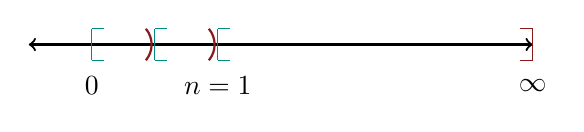
\begin{tikzpicture}[scale=0.8]
        \def\cdraw{Cyan4}
        \def\ddraw{Firebrick4}
        \def\bound{7}
        \def\n{1}
        \def\radius{0.25}
        \def\avlen{0.2}
        \pgfmathparse{\n * 2^\n}
        \let\maxi\pgfmathresult
        \pgfmathparse{\radius / sin(40)}
        \let\circr\pgfmathresult
        \pgfmathparse{\circr * cos(40)}
        \let\circx\pgfmathresult

        \draw[<->, black, thick] (-1,0) -- (\bound,0);
        \node at (0, -\radius -0.4) {$0$};
        \foreach \i in {1,...,\maxi} {
            \pgfmathparse{2*(\i -1)/(2^\n)}
            \let\lbound\pgfmathresult
            \pgfmathparse{2*(\i)/(2^\n)}
            \let\rbound\pgfmathresult
            
            
            \draw[-, \cdraw] (\lbound, -\radius) -- (\lbound, \radius);
            \draw[-, \cdraw] (\lbound, \radius) -- (\lbound + \avlen, \radius);           
            \draw[-, \cdraw] (\lbound, -\radius) -- (\lbound + \avlen, -\radius);
            
            \draw[-, \ddraw, thick] (\rbound - \circr + \circx - 0.05, \radius) arc [start angle =40, end angle = -40, radius=\circr];
        }
        \draw[-, \cdraw] (2*\n, -\radius) -- (2*\n, \radius);
        \draw[-, \cdraw] (2*\n, \radius) -- (2*\n + \avlen, \radius);           
        \draw[-, \cdraw] (2*\n, -\radius) -- (2*\n + \avlen, -\radius);
        \draw[-, \ddraw] (\bound, -\radius) -- (\bound, \radius);
        \draw[-, \ddraw] (\bound, \radius) -- (\bound - \avlen, \radius);           
        \draw[-, \ddraw] (\bound, -\radius) -- (\bound - \avlen, -\radius);
        \node at (2*\n, -\radius -0.4) {$n=\n$};
        \node at (\bound, -\radius -0.4) {$\infty$};
    \end{tikzpicture}
    \end{center}
\end{minipage}
\begin{minipage}{0.5\textwidth}
\begin{center}
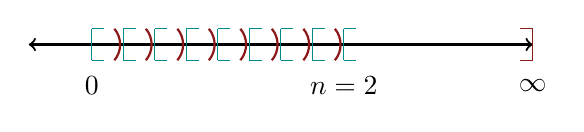
\begin{tikzpicture}[scale=0.8]
    \def\cdraw{Cyan4}
    \def\ddraw{Firebrick4}
    \def\bound{7}
    \def\n{2}
    \def\radius{0.25}
    \def\avlen{0.2}
    \pgfmathparse{\n * 2^\n}
    \let\maxi\pgfmathresult
    \pgfmathparse{\radius / sin(40)}
    \let\circr\pgfmathresult
    \pgfmathparse{\circr * cos(40)}
    \let\circx\pgfmathresult

    \draw[<->, black, thick] (-1,0) -- (\bound,0);
    \node at (0, -\radius -0.4) {$0$};
    \foreach \i in {1,...,\maxi} {
        \pgfmathparse{2*(\i -1)/(2^\n)}
        \let\lbound\pgfmathresult
        \pgfmathparse{2*(\i)/(2^\n)}
        \let\rbound\pgfmathresult
        
        
        \draw[-, \cdraw] (\lbound, -\radius) -- (\lbound, \radius);
        \draw[-, \cdraw] (\lbound, \radius) -- (\lbound + \avlen, \radius);           
        \draw[-, \cdraw] (\lbound, -\radius) -- (\lbound + \avlen, -\radius);
        
        \draw[-, \ddraw, thick] (\rbound - \circr + \circx - 0.05, \radius) arc [start angle =40, end angle = -40, radius=\circr];
    }
    \draw[-, \cdraw] (2*\n, -\radius) -- (2*\n, \radius);
    \draw[-, \cdraw] (2*\n, \radius) -- (2*\n + \avlen, \radius);           
    \draw[-, \cdraw] (2*\n, -\radius) -- (2*\n + \avlen, -\radius);
    \draw[-, \ddraw] (\bound, -\radius) -- (\bound, \radius);
    \draw[-, \ddraw] (\bound, \radius) -- (\bound - \avlen, \radius);           
    \draw[-, \ddraw] (\bound, -\radius) -- (\bound - \avlen, -\radius);
    \node at (2*\n, -\radius -0.4) {$n=\n$};
    \node at (\bound, -\radius -0.4) {$\infty$};
\end{tikzpicture}
\end{center}
\end{minipage}
\\[5mm]
Conjuntos inducidos para los casos $n=1$ y $n = 2$.

\vspace{2mm} Sea $x_0 \in X$ cualquiera, dependiendo del valor de $f(x_0)$ pueden darse dos casos:

\vspace{2mm} $\bullet$ Si $f(x_0) = +\infty$, $f(x_0) \in [n, +\infty]$ $\hspace{1mm} \forall \hspace{1mm} n \in \N$, luego $s_n(x_0) = n \xrightarrow{n\to\infty} \infty = f(x_0)$ de manera creciente.

\newpage $\bullet$ Si $f(x_0) \in (0, +\infty)$, podemos tomar $m := \min\{n \in \N : n > f(x_0)\}$.
Así, se cumple $s_1(x_0) = 1 < s_2(x_0) = 2 < \ldots < s_{m-1}(x_0) = m-1 < s_m(x_0) < m$.

\vspace{4mm} Para $n \geq m$, tenemos que $ \exists ! i_n \in \{1,\ldots, n\cdot 2^n\}$ que verifica: $$f(x_0) \in \left[\frac{i_n-1}{2^n}, \frac{i_n}{2^n}\right) = \left[\frac{2i_n-2}{2^{n+1}}, \frac{2i_n-1}{2^{n+1}}\right) \cup \left[\frac{2i_n-1}{2^{n+1}}, \frac{2i_n}{2^{n+1}}\right)$$
De este modo, $s_n(x_0) = \frac{i_n - 1}{2^n}$ y además $s_{n+1}(x_0) \in \left\{\frac{2i_n-2}{2^{n+1}}, \frac{2i_n-1}{2^{n+1}}\right\}$ luego ha de cumplirse necesariamente $s_n(x_0) \leq s_{n+1}(x_0)$. Al ser una sucesión no decreciente y acotada, podemos afirmar que $\exists \hspace{1mm} l := \mlim{n} s_n(x_0) \in (0, +\infty)$. Veamos que $l = f(x_0)$. Dado $n \geq m$, se cumple:
\begin{flalign*}
    s_n(x) = \frac{i_n - 1}{2^n} \leq f(x_0) < \frac{i_n}{2^n} = \frac{i_n - 1}{2^n} + \frac{1}{2^n} = s_n(x_0) + \frac{1}{2^n}
\end{flalign*}
Tomando límites cuando $n \to \infty$, concluimos que $l \leq f(x_0) \leq l$.

\vspace{6mm}
\result{Convergencia uniforme para funciones acotadas}
\hspace{3mm} Sea $(X, \Sigma, \mu)$ un espacio de medida. Sea $f : X \longrightarrow [0, +\infty)$ una función medible y acotada. Entonces existe una sucesión de funciones simples $s_n : X \longrightarrow [0, \infty)$ tales que:
\begin{enumerate}[label=\roman*)]
    \item $\forall \hspace{1mm}  n \in \N $ $\forall \hspace{1mm} x \in X : $ $ s_n(x) \leq s_{n+1}(x)$
    \item $ s_n \xrightarrow{u} f$
\end{enumerate}
\nota Podemos suponer que $f$ está estrictamente acotada por $1$. En caso contrario, estará estrictamente acotada por cierto $K \in (0,+\infty)$. Podemos aplicar el resultado a $\frac{f}{K}$, que estará acotada por $1$, y multiplicar las funciones simples por $K$ con el fin de que se cumpla para la $f$ original.

\vspace{2mm} \dem

\vspace{2mm} En vista del \hyperref[result:1.3.17]{resultado anterior}, queda comprobar que la convergencia es uniforme. Siguiendo la notación de la demostración anterior,
$$s_n = n \cdot X_{E_n} + \sum_{i = 1}^{n \cdot 2^n} \left(\frac{i-1}{2^n} \cdot X_{E_{n,i}}\right)$$
Al suponer que $f$ está estrictamente acotada por $1$, el primer sumando es siempre nulo. Por tanto, para todo $n \in \N$ se cumple $E_n = f^{-1}\Big([n, +\infty]\Big) = \varnothing$, $\forall \hspace{1mm} x \in X : f(x) \in \left[\frac{i_{n,x}-1}{2^n}, \frac{i_{n,x}}{2^n}\right)$ para cierto $i_{n,x} \in \{1,\ldots, n\cdot 2^n\}$. De este modo,
$$\left|s_n(x) - f(x)\right| \leq \frac{1}{2^n} \xrightarrow{n\to\infty} 0 \hspace{2mm} \text{ uniformemente para cualquier } x \in X$$

\newpage
\unit{Integral de Lebesgue}
\chapter{Integral de Lebesgue para funciones no negativas}
\result{Convenio \texorpdfstring{$0 \cdot \infty$}{0 · infty}}
\hspace{3mm} Consideramos $0 \cdot \infty = 0$ siempre y cuando al menos uno de los dos factores represente la medida de algún conjunto.

\hspace{4mm}
\result{Definición de integral de funciones simples}
\hspace{3mm} Dado un espacio de medida $(X, \Sigma, \mu)$ y una función simple medible
\begin{align*}
    s: X \longrightarrow [0, +\infty) && \text{ con expresión canónica } s = \sum_{i = 1}^n \lambda_i X_{A_i}
\end{align*}
Definimos la integral de Lebesgue de $s$ sobre $X$ como el número:
$$\lbint_X s \,d\mu = \sum_{i=1}^{n} \lambda_i \cdot \mu(A_i)$$

\nota Implícitamente, ya está definida la integral de $s$ sobre $\Sigma(E) \hspace{2mm } \forall \hspace{1mm} E \in \Sigma$:
$$\lbint_E s \,d \mu = \lbint_X s_{|E} \,d\mu = \sum_{i=1}^{n}\lambda_i \cdot \mu(E \cap A_i)$$

\newpage
\result{Linealidad del integrando}
\hspace{3mm} Dado un espacio de medida $(X, \Sigma, \mu)$. Sea $s: X \longrightarrow [0, \infty)$ una función simple y medible. Sean $\{E_i\}_{i\in\N} \subseteq \Sigma$ con $i \neq j \Rightarrow E_i \cap E_j = \varnothing$. Entonces, se cumple:
$$\lbint_{\smallcup_{i\in\N}E_i} s \, d\mu = \sum_{i=1}^\infty \lbint_{E_i}s\,d\mu$$

\vspace{3mm}
\dem Sea $s = \displaystyle \sum_{i=1}^{n} \lambda_i \cdot X_{A_i}$ la expresión canónica de $s$. Entonces,
\begin{flalign*}
    &\lbint_{\smallcup_{i\in\N}E_i}s\,d\mu = \sum_{i=1}^{n} \lambda_i \cdot \mu\big(A_i \cap \smallcup_{i\in\N}E_i\big) = \sum_{i=1}^n \lambda_i \sum_{j=1}^\infty \mu(A_i \cap E_j) = \\
    &= \sum_{i=1}^n \left(\sum_{j=1}^\infty \lambda_i \cdot \mu(A_i \cap E_j) \right) = \sum_{j=i}^\infty \sum_{i=1}^n \lambda_i \cdot \mu(A_i \cap E_j) = \sum_{j=1}^{\infty} \lbint_{E_j}s\,d\mu
\end{flalign*}

\vspace{6mm}
\result{Linealidad parcial}
\hspace{3mm} Sea $(X, \Sigma, \mu)$ un espacio de medida. Sean $s,t : X \longrightarrow [0, \infty)$ funciones simples y medibles. Entonces, se cumple:
$$\lbint_{X}s + t\,d\mu = \lbint_{X}s\,d\mu + \lbint_{X}t\,d\mu$$

\vspace{2mm} \dem Sean sus expresiones canónicas las siguientes:
\begin{align*}
    s = \sum_{i=1}^{n} \alpha_i \cdot X_{A_i} && t = \sum_{j=1}^m \beta_j \cdot X_{B_j}
\end{align*}
Entonces, como $\{A_i\}_{i=1}^n$ y $\{B_j\}_{j=1}^m$ son recubrimientos disjuntos de $X$, se tiene:
\begin{flalign*}
    \lbint_{X}s\,d\mu = \sum_{i=1}^n \alpha_i \sum_{j=1}^{m} \mu(A_i \cap B_j) = \sum_{\substack{1\leq i \leq n \\ 1 \leq j \leq m}} \alpha_i \cdot \mu(A_i \cap B_j) \\
    \lbint_{X}t\,d\mu = \sum_{j=1}^m \beta_j \sum_{i=1}^{n} \mu(A_i \cap B_j) = \sum_{\substack{1\leq i \leq n \\ 1 \leq j \leq m}} \beta_j \cdot \mu(A_i \cap B_j)
\end{flalign*}
Sumando ambas expresiones obtenemos:
\begin{flalign*}
    \lbint_{X}&s\,d\mu + \lbint_{X}t\,d\mu = \sum_{\substack{1\leq i \leq n \\ 1 \leq j \leq m}} (\alpha_i + \beta_j) \cdot \mu(A_i \cap B_j) = \\
    &= \sum_{\substack{1\leq i \leq n \\ 1 \leq j \leq m}} \lbint_{A_i \cap B_j}s + t\,d\mu = \lbint_{X}s+t\,d\mu
\end{flalign*}
La última igualdad se deduce de la \hyperref[result:2.1.3]{linealidad del integrando}.

\hspace{4mm}
\result{Monotonía de la integral simple}
\hspace{3mm} Sea $(X, \Sigma, \mu)$ un espacio de medida. Sean $s, t: X \longrightarrow [0, \infty)$ funciones medibles simples tales que $s(x) \leq t(x) \hspace{2mm} \forall x \in X$. Entonces, se cumple:
$$\lbint_{X}s\,d\mu \leq \lbint_{X}t\,d\mu$$

\vspace{2mm} \dem Sean sus expresiones canónicas: $\displaystyle s= \sum_{i=1}^n \alpha_i \cdot X_{A_i} \hspace{3mm} t = \sum_{j=1}^m \beta_j \cdot X_{B_j}$.
\begin{align*}
    \lbint_{X}s\,d\mu = \sum_{\substack{1\leq i \leq n\\1\leq j \leq m}} \alpha_i \mu(A_i \cap B_j) &&
    \lbint_{X}t\,d\mu = \sum_{\substack{1\leq i \leq n\\1\leq j \leq m}} \beta_j \mu(A_i \cap B_j)
\end{align*}
\indent Por hipótesis, tenemos que $s(x) \leq t(x)$ para todo $x\in X$. De este modo; sean $i \in \{1,\ldots,n\}, j \in \{1,\ldots, m\}$ cualesquiera, tenemos que o bien $\alpha_i \leq \beta_j$ o bien $A_i \cap B_j = \varnothing \Rightarrow \mu(A_i \cap B_j) = 0$. Por tanto, cada sumando del sumatorio de la izquierda va a ser menor o igual que el término de mismos índices del sumatorio de la derecha, hemos demostrado el resultado.

\vspace{6mm}
\result{Linealidad de la integral simple por constantes}
\hspace{3mm} Sea $(X, \Sigma, \mu)$ un espacio de medida. Sea $\displaystyle s = \sum_{i=1}^n \lambda_i \cdot X_{A_i}$ una función simple, medible y no negativa. Entonces:
$$\lbint_{X}c \cdot s\,d\mu = c \cdot \lbint_{X}s\,d\mu \hspace{4mm} \forall c \in \R$$
\vspace{2mm} \dem Distinguimos dos casos:
\begin{itemize}
    \item Si $c = 0$, entonces $s \cdot c \equiv 0$ y se cumple:
    $$\lbint_{X}c \cdot s\,d\mu = \lbint_{X}0\,d\mu = 0 \cdot \mu(X) = 0 = 0 \cdot \lbint_{X}s\,d\mu$$
    \item Si $c \neq 0$, entonces:
    $$\lbint_{X}c\cdot s\,d\mu = \sum_{i=1}^{n} c \cdot \lambda_i \cdot \mu(A_i) = c \cdot \sum_{i=1}^n \lambda_i \cdot \mu(A_i) = c \cdot \sum_{i=1}^n \lambda_i \cdot \mu(A_i) = c \cdot \lbint_{X}s\,d\mu $$
\end{itemize}

\vspace{6mm}
\result{Integral de funciones medibles no negativas}
\hspace{3mm} Sea $(X, \Sigma, \mu)$ un espacio de medida. Sea $f : X \longrightarrow [0, +\infty]$ medible. Se define la integral de Lebesgue de $f$ sobre $X$ como:
$$\int_{X}f\,d\mu = \sup\left\{\lbint_{X}s\,d\mu \hspace{2mm} \text{ con } 0 \leq s \leq f, \hspace{1mm} s \hspace{1mm} \substack{\text{ función simple medible}\\[1ex] s < \infty}\right\} = \sup \mathcal{S}_X(f)$$
Nótese que el conjunto anterior no es vacío, pues $s \equiv 0$ está en él. Además, se puede extender la definición anterior a cualquier subconjunto medible de $X$.

\vspace{6mm}
\result{Ejemplos de integrales}
\hspace{3mm} $\romannumeral 1)$ Función de Dirichlet: $X_\Q$. \newline Consideramos el espacio de medida $\big([0,1], \mathfrak{M}_1([0,1]), \mu_1\big)$. Esta función no es integrable en el sentido de Riemann, pues las sumas inferiores son siempre nulas y las superiores toman valor $1$ (se debe a la densidad de los racionales y los irracionales). Veamos que $X_\Q$ sí es integrable en el sentido de Lebesgue.
\newline \vspace{4mm} \indent Tenemos que $X_\Q$ es una función simple, pues toma el valor $1$ en $[0,1]\cap \Q$, que es numerable, y el valor $0$ en $[0,1]\setminus \Q$, que es medible al ser el complementario del conjunto anterior en este espacio de medida. Su integral viene dada por:
$$\lbint_{[0,1]}X_\Q\,d\mu = 1 \cdot \mu([0,1] \cap \Q) + 0 \cdot \mu([0,1] \setminus \Q) = 1 \cdot 0 + 0 \cdot 1 = 0$$
\vspace{4mm} \indent $\romannumeral 2)$ Consideramos el mismo espacio de medida que en el caso anterior. Veamos que la función de Thomae es integrable. Se define como sigue:
$$f(x) = \begin{cases}
    0 &\text{ si } x \in \Q\cap[0,1] \cup \{0\} \\
    \frac{1}{q} &\text{ si } x = \frac{p}{q} \text{ para }p,q \text{ naturales primos entre sí}
\end{cases} $$
\indent Sabemos por Análisis Matemático II que esta función es integrable-Riemann en $[0,1]$ con valor de su integral igual a $0$. Veamos que ocurre lo mismo con la integral de Lebesgue. Sea $s$ una función simple medible tal que $0 \leq s \leq f$. Se cumple $M := \max s([0,1]) \leq 1$. Los puntos donde $s$ toma valores positivos son a lo sumo numerables, pues se cumple:
$$f^{-1}\big((0, +\infty)\big) = \bigcup_{n\in\N} \hspace{1mm}\bigcup_{i=1}^n \frac{i}{n}$$
Los puntos donde $s$ toma valores positivos han de estar contenidos en el conjunto anterior, que es numerable y tiene por tanto medida nula. De este modo, tenemos:
$$0 \leq \lbint_{[0,1]}s\,d\mu = 0 \cdot \mu\big(s^{-1}(\{0\})\big) + M \cdot \mu\Big(s^{-1}\big((0,M]\big)\Big) = 0$$

\vspace{6mm} \result{Propiedades básicas}
\hspace{3mm}  Sea $(X, \Sigma, \mu)$ un espacio de medida. Sean $f,g : X \rightarrow [0, \infty]$ funciones medibles. Sean $E,F \in \Sigma$. Sea $c \in [0, +\infty)$. Se cumplen los siguientes enunciados:
\begin{enumerate}[label=\roman*)]
    \item $0 \leq f \leq g \Rightarrow \int_{X}f\,d\mu \leq \int_{X}g\,d\mu$
    \item $\int_{X}c \cdot f\,d\mu = c \cdot \int_{X}f\,d\mu$
    \item $f\equiv 0 \Rightarrow \int_{X}f\,d\mu = 0$
    \item $\mu(E) = 0 \Rightarrow \int_{E}f\,d\mu = 0$
    \item Si $E \subseteq F$; entonces, $\int_{E}f\,d\mu = \int_{F}f \cdot X_E\,d\mu$ y $\int_{E}f\,d\mu \leq \int_{F}f\,d\mu$
\end{enumerate}
\vspace{2mm} \dem \newline \vspace{2mm} $\romannumeral 1)$ Sea $s : X \longrightarrow [0, +\infty)$ una función simple medible tal que $s \leq f$. Entonces se cumple $s \leq g$. Por tanto, siguiendo la notación del \hyperref[result:2.1.7]{resultado 2.1.7}, tenemos que $\mathcal{S}_X(f) \subseteq \mathcal{S}_X(g)$ luego ha de cumplirse: $$\int_{X}f\,d\mu = \sup \mathcal{S}_X(f) \leq \sup \mathcal{S}_X(g) = \int_{X}g\,d\mu$$

\vspace{4mm} $\romannumeral 2)$ Distinguimos dos casos: En primer lugar, si $c = 0$ se tiene: $$\int_{X}c \cdot f\,d\mu = \int_{X}0\,d\mu = 0 = 0 \cdot \int_{X}f\,d\mu$$
Si $c \in (0, +\infty)$; entonces, tenemos:
\begin{flalign*}
    c \cdot \int_{X}f\,d\mu & = c \cdot \sup \left\{\lbint_{X}s\,d\mu : \hspace{2mm} 0 \leq s \leq f \hspace{2mm} \text{ con } s \text{ función medible simple}\right\} = c \cdot \sup \mathcal{S}_X(f)\\
    \int_{X}c\cdot f\,d\mu & \sup \left\{\lbint_{X}t\,d\mu : \hspace{2mm} 0 \leq t \leq c\cdot f \hspace{2mm} \text{ con } t \text{ función medible simple}\right\} = \sup \mathcal{S}_X(c\cdot f)
\end{flalign*}
Al cumplirse $c \in (0,+\infty)$, tenemos que $0 \leq f \leq s \iff 0 \leq c \cdot s \leq c \cdot f$ luego las integrales han de coincidir.

\vspace{6mm} $\romannumeral 3$  $\romannumeral 4)$ Trivial.

\vspace{4mm} $\romannumeral 5)$ Comencemos por ver la primera parte. Sea una función simple y medible $s : F \longrightarrow [0, +\infty)$ tal que $s \leq f \cdot X_E$. Entonces se tiene $s_{|E}$ es simple también. Además, se cumple:
$$\lbint_{F}s\,d\mu = \lbint_{E}s_{|E}\,d\mu + \lbint_{F \setminus E}0\,d\mu = \int_{E}s_{|E}\,d\mu$$
De manera similar, sea $t : E \longrightarrow [0,+\infty)$ simple tal que $t \leq f$, podemos extender $t$ a $F$ al considerar $\hat{t}(x) = t(x)$ si $x \in E$ ó $0$ si $x \in F \setminus E$. La función resultante $\hat{t}$ es simple, medible y cumple $\hat{t} \leq f \cdot X_E$. De este modo,
$$\lbint_{F}\hat{t}\,d\mu = \int_{F \setminus E}0\,d\mu + \lbint_{E}\hat{t}\,d\mu = \lbint_{E}t\,d\mu$$
Por tanto, se cumple $\mathcal{S}_E(f) = \mathcal{S}_F(f \cdot X_E)$ luego las integrales coinciden.
\vspace{4mm} \newline \indent Este razonamiento de extender $t$ a $\hat{t}$ demuestra también que $\mathcal{S}_E(f) \subseteq \mathcal{S}_F(f)$ luego por definición de supremo, se tiene:
$$\int_{E}f\,d\mu = \sup \mathcal{S}_E(f) \leq \sup \mathcal{S}_F(f) = \int_{F}f\,d\mu$$
Se cumple también la segunda parte.

\vspace{6mm}
\result{Teorema de la convergencia monótona}
\hspace{3mm} Dado un espacio de medida $(X, \Sigma, \mu)$. Sea $\{f_n : X \longrightarrow [0, +\infty]\}_{n\in\N}$ una sucesión de funciones medibles tales que:
\begin{align*}
    \forall \hspace{1mm} x \in X \hspace{2mm} \forall n \in \N : f_n(x) \leq f_{n+1}(x) && f_n(x) \xrightarrow{n\to\infty} f(x)
\end{align*}
Entonces, existe el límite de las integrales y coincide con la integral de la función límite:
$$\lim_n \int_{X}f_n\,d\mu = \int_{X}\lim_n f_n\,d\mu = \int_{X}f\,d\mu$$
\vspace{2mm} \dem

\vspace{2mm} Como $f_n \leq f_{n+1}$ por hipótesis para todo $n \in \N$. Aplicando la \hyperref[result:2.1.9]{monotonía de la integral}, tenemos:
\begin{flalign*}
    \int_{X}f_n\,d\mu \leq \int_{X}f_{n+1}\,d\mu \Rightarrow \exists \hspace{1mm} \lim_n \int_{X}f_n\,d\mu = \alpha \in [0, +\infty]
\end{flalign*}
Al ser una sucesión monótona, o bien converge o diverge. Es por ello que podemos garantizar la existencia del límite, $\alpha$.
\vspace{2mm} \newline \indent Como $f_n(x) \xrightarrow{n\to\infty} f(x)$ de manera creciente para todo $x \in X$, para cada $n \in \N$ tenemos $f_n \leq f \Rightarrow \int_{X}f_n\,d\mu \leq \int_{X}f\,d\mu \Rightarrow \alpha \leq \int_{X}f\,d\mu$. Queda demostrar $\int_{X}f\,d\mu \leq \alpha$. Para ello, sea $s : X \longrightarrow [0, +\infty]$ una función simple y medible con $s \leq f$, basta ver que $\lbint_{X}s\,d\mu \leq \alpha$.
\vspace{4mm} \newline \indent Sea $\hspace{1mm} c \in [0, 1)$. Para cada $x \in X$ existe $n_x \in \N$ tal que $c \cdot s(x) \leq f_n(x) \leq f(x) \hspace{2mm} \forall n \geq n_x$. Podemos suponer sin pérdida de generalidad que $s(x) < \infty$ para aquellos $x$ con $f(x) = \infty$ par que se cumpla el razonamiento anterior. Para cada $n \in \N$, consideramos el siguiente conjunto:
%TODO preguntar en clase
$$E_n :=  \{x \in X : c \cdot s(x) \leq f_k(x) \leq f(x) \hspace{2mm} \forall k \geq n \} \hspace{2mm} \in \Sigma$$
Al ser $s, f_n, f$ medibles, podemos garantizar que $E_n$ es medible. Por definición, es claro que $E_n \subseteq E_{n+1}$ Además, se tiene $x \in X \Rightarrow x \in E_{n_x} \Rightarrow X = \smallcup_{n\in\N} E_n$.
\vspace{4mm} \newline \indent Sea $\displaystyle s = \sum_{i = 1}^{m} \lambda_i \cdot X_{A_i}$ la expresión canónica de $s$, se cumple:
\begin{flalign*}
    \int_{E_n}c \cdot s\,d\mu \leq \int_{E_n}f_n\,d\mu \leq \int_{E_n}f\,d\mu
\end{flalign*}
Pero por definición de integral simple, se cumple:
$$\int_{E_n}c \cdot s\,d\mu = c \cdot \sum_{i=1}^m \lambda_i \cdot \mu(E_n \cap A_i) \xrightarrow{n \to \infty} c \cdot \sum_{i=1}^m \lambda_i \cdot \mu(A_i) = c\cdot \int_{X}s\,d\mu$$
De este modo, tomando límites en la desigualdad anterior, $c \cdot \int_{X}s\,d\mu \leq \alpha$. Tomando $\mlim{c \to 1^-}$ concluimos que $\int_{X}s\,d\mu \leq \alpha$.

\vspace{6mm}
\result{Integral de la suma}
\hspace{3mm} Sea $(X, \Sigma, \mu)$ un espacio de medida. Sean $f,g : X \longrightarrow [0,+\infty]$ funciones medibles. Entonces, se cumple:
$$\int_{X}f\,d\mu + \int_{X}g\,d\mu = \int_{X}f+g\,d\mu$$
\vspace{2mm}\dem \vspace{2mm} \newline Podemos afirmar que existe una colección de funciones simples y medibles $\{s_n,t_n:X \longrightarrow [0,+\infty]\}_{n\in\N}$ tales que para todo $x \in X$ para todo $n \in \N$ se cumpla:
\begin{align*}
    s_n(x) \leq s_{n+1}(x) \leq f && t_n(x) \leq t_{n+1}(x) \leq g &&
    s_n(x) \xrightarrow{n\to\infty} f(x) && t_n(x) \xrightarrow{n\to\infty} g(x)
\end{align*}
Entonces, tenemos que $s_n + t_n \leq s_{n+1} + t_{n+1}$ y además $(s_n + t_n)(x) \xrightarrow{n\to\infty} (f+g)(x)$. Aplicando el \hyperref[result:2.1.10]{Teorema de la Convergencia Monótona}, tenemos:
\begin{align*}
    \int_{X}f\,d\mu + \int_{X}g\,d\mu = \lim_n \int_{X}s_n\,d\mu + \lim_n \int_{X}t_n\,d\mu = \lim \int_{X}s_n + t_n\,d\mu = \int_{X}f + g\,d\mu
\end{align*}

\vspace{6mm}
\result{Integrales en conjuntos disjuntos}
\hspace{3mm} Sea $(X, \Sigma, \mu)$ un espacio de medida. Sea $f : X \longrightarrow [0, +\infty]$ una función medible. Sean $\{E_i\}_{i\in\N} \subseteq \Sigma$ con $i \neq j \Rightarrow E_i \cap E_j = \varnothing$. Entonces, se cumple:
$$ \int_{\smallcup_{i\in\N} E_i}f\,d\mu = \sum_{i=1}^{\infty} \int_{E_i}f\,d\mu$$
\vspace{2mm} \dem
\begin{flalign*}
    \mathop{\int}_{\smallcup_{i=1}^n E_i}f\,d\mu = \int_{X}f \cdot X_{\smallcup_{i=1}^n E_i}\,d\mu = \int_{X}\sum_{i=1}^{n}f \cdot X_{E_i} \,d\mu \overset{\hyperref[result:2.1.11]{2.1.11}}{=} \sum_{i=1}^{n} \int_{X}f \cdot X_{E_i}\,d\mu
\end{flalign*}
Tomando límites llegamos al resultado:
\begin{flalign*}
    \mathop{\int}_{\smallcup_{i\in\N}E_i}f\,d\mu = \int_{X}\sum_{i=1}^{\infty} f \cdot X_{E_i}\,d\mu = \sum_{i=1}^{\infty} \int_{X}f \cdot X_{E_i}\,d\mu = \sum_{i=1}^{\infty} \int_{E_i}f\,d\mu
\end{flalign*}

\vspace{6mm}
\result{Lema de Fatou}
\hspace{3mm} Sea $(X, \Sigma, \mu)$ un espacio de medida. Sea una sucesión de funciones medibles $\{f_n : X \longrightarrow [0, +\infty]\}_{n\in\N}$. Entonces, se cumple:
$$\int_{X}\linf{n} f_n\,d\mu \leq \linf{n} \int_{X}f_n\,d\mu$$
\vspace{2mm} \dem \vspace{2mm} \newline \indent Por definición, $\linf{n} f_n = \mlim{n} \inf_{k \geq n} f_k(x) = \mlim{n} g_n(x)$ Para $g_n$ medible. Además, $g_n \leq g_{n+1}$. De este modo, estamos en condiciones de aplicar el \hyperref[result:2.1.10]{Teorema de la Convergencia Monótona}:
\begin{flalign*}
    \int_{X} \linf{n} f_n\, d\mu
    = \int_{X} \lim_{n} g_n\, d\mu
    = \lim_{n} \int_{X} g_n\, d\mu
    \overset{(*)}{\leq} \linf{n} \int_{X} f_n\, d\mu
\end{flalign*}
(*) Como $g_n \leq f_n$, tenemos que $g_{k_n} \leq f_{k_n}$ (y por tanto $\int_{X}g_{k_n}\,d\mu \leq \int_{X}f_{k_n}\,d\mu$) para cualquier subsucesión; en particular, para la sucesión que tiene como límite el límite inferior.

\vspace{2mm}
\nota En general, la igualdad no tiene por qué cumplirse:
\begin{align*}
    f_n = X_{[n, +\infty)} &&
    \int_{\R}\lim_n f_n\,d\mu_1 = \int_{\R}0\,d\mu_1 = 0 &&
    \int_{\R}f_n\,d\mu_1 = \infty \xrightarrow{n\to\infty}\infty
\end{align*}

\vspace{6mm}
\result{Definición de igualdad en casi todo punto}
\hspace{3mm} Sea $(X, \Sigma, \mu)$ un espacio de medida. Sean dos funciones $f,g : X \longrightarrow \overline{\R}$. Se dice que $f$ y $g$ ``son iguales en casi todo punto'' si $\exists B \in \Sigma$ con $\mu(B) = 0$ tal que:
$$\{x \in X : f(x) \neq g(x)\} \subseteq B$$
En tal caso, se denotará como $f \overset{\mu-a.e.}{=} g$ ó $f = g \hspace{1mm} \mu-a.e.$, las letras ``a.e.'' vienen del término inglés ``\textit{almost everywhere}''.

\vspace{6mm}
\result{Medibilidad de funciones iguales en casi todo punto}
\hspace{3mm} Sea $(X, \Sigma, \mu)$ un espacio de medida completo. Sean $f,g : X \longrightarrow \overline{\R}$ funciones tales que $f \overset{\mu-a.e.}{=}g$. Si $f$ es medible; entonces, $g$ es medible también.
\vspace{4mm} \dem \vspace{2mm} \newline \indent Sea $A := \{x \in X : f(x) \neq g(x)\}$. Por hipótesis, $f \overset{\mu-a.e.}{=} g$ luego $\exists \hspace{1mm} B \in \Sigma$ con $\mu(B) = 0$ tal que $A \subseteq B$. Al ser $(X, \Sigma, \mu)$ completo por hipótesis, tenemos que $A \in \Sigma$ también. De este modo, sea $\alpha \in \R$ cualquiera,
\begin{flalign*}
    \{x \in X : g(x) < \alpha\} = \underbracket{\{x\in X : f(x) < \alpha\}\cap (X \setminus A)}_{\in\Sigma} \hspace{1mm} \cup \hspace{1mm} \underbracket{\{x \in X : g(x) < \alpha\} \cap A}_{\in \Sigma} \in \Sigma
\end{flalign*}
El primer subconjunto es medible al ser $f$ medible por hipótesis. El segundo conjunto es medible al tener también medida nula por ser un subconjunto de $A$.

\vspace{6mm}  
\result{Integral de funciones iguales en casi todo punto}
\hspace{3mm} Sea $(X, \Sigma, \mu)$ un espacio de medida. Sean $f,g : X \longrightarrow [0, +\infty]$ funciones medibles. Entonces, se cumple:
$$ f \overset{\mu-a.e.}{=} g \Rightarrow \int_{X}f\,d\mu = \int_{X}g\,d\mu$$
\vspace{2mm} \dem \vspace{2mm} Por ser $f,g$ medibles, $A:= \{x \in X : f(x) \neq g(x)\} \in \Sigma$. Además, $f \overset{\mu-a.e.}{=}g$ luego $\mu(A) = 0$. De este modo,
\begin{flalign*}
    \int_{X}&f\,d\mu = \int_{X \setminus A}f\,d\mu + \int_{A}f\,d\mu = \int_{X \setminus A}f\,d\mu + 0 = \\
    &= \int_{X \setminus A}g\,d\mu + 0 = \int_{X \setminus A}g\,d\mu + \int_{A}g\,d\mu = \int_{X}g\,d\mu
\end{flalign*}
\nota Este resultado será también válido para funciones de signo variable.

\vspace{6mm}
\result{Integral de funciones nulas en casi todo punto}
\hspace{3mm} Sea $(X, \Sigma, \mu)$ un espacio de medida. Sea $f : X \longrightarrow [0, +\infty]$ una función medible. Entonces,
$$f \overset{\mu-a.e.}{=} 0 \iff \int_{X}f\,d\mu = 0$$
\vspace{2mm}\dem
\begin{tcolorbox}[Subset-contingency]
    $\Rightarrow$ \hspace{2mm} Se tiene como aplicación directa del \hyperref[result:2.1.16]{resultado anterior}.
\end{tcolorbox}
\begin{tcolorbox}[Subset-contingency]
    $\Leftarrow$ \hspace{2mm} Para cada $n \in \N$ tomamos $E_n := \{x \in X : f(x) \geq \frac{1}{n}\} \hspace{2mm} \overset{f \text{ medible}}{\in} \Sigma$.
\end{tcolorbox}
Sea $E := \smallcup_{n\in\N}E_n \in \Sigma$. Entonces, para cada $n \in \N$ se cumple:
$$0 \leq \frac{1}{n} \cdot \mu(E_n) = \int_{X}\frac{1}{n} \cdot X_{E_n}\,d\mu \leq \int_{E_n}f\,d\mu \leq \int_{X}f\,d\mu = 0$$
Por tanto, $\mu(E_n) = 0$ luego $\mu(E) \leq \displaystyle \sum_{n=1}^\infty \mu(E_n) = 0 \Rightarrow f \overset{\mu-a.e.}{=} 0$.
\vspace{4mm}\newline\nota
\begin{tcolorbox}[Subset-contingency]
    $\Rightarrow$ \hspace{2mm} La implicación es válida para $f : X \longrightarrow \overline{\R}$.
\end{tcolorbox}
\begin{tcolorbox}[Subset-contingency]
    $\Leftarrow$ \hspace{2mm} Es necesario exigir $f \geq 0$. Por ejemplo, $\int_{[0,2\pi]}\sin(x)\,d\mu(x) = 0$.
\end{tcolorbox}

\newpage
\chapter{Integral de Lebesgue para funciones \texorpdfstring{$f:x \longrightarrow \overline{\R}$}{f : X -> R}}
\result{Funciones integrables y sumables}
\hspace{3mm} Sea $(X, \Sigma, \mu)$ un espacio de medida. Sea $f : X \longrightarrow \overline{\R}$ medible. Diremos que ``$f$ es integrable sobre $X$'' si cumple cualquiera de las siguientes dos condiciones:
\begin{align*}
    \int_{X}f^+\,d\mu < \infty && \int_{X}f^-\,d\mu < \infty
\end{align*}
Si $f$ cumple simultáneamente ambas condiciones, diremos que ``$f$ es sumable'' (toda función sumable es integrable). En cualquier caso, podemos definir la integral de $f$ sobre $X$ como:
$$\int_{X}f\,d\mu = \int_{X}f^+\,d\mu - \int_{X}f^-\,d\mu$$
Nótese que como consecuencia inmediata de las definiciones anteriores, los siguientes enunciados son equivalentes:
\begin{enumerate}[label=\roman*)]
    \item $f$ sumable
    \item $f^+$ y $f^-$ sumables
    \item $|f|$ sumable
    \item $\int_{\R}f\,d\mu \in \R$
    \item $\int_{\R}|f|\,d\mu \in \R$
\end{enumerate}

\vspace{6mm}
\result{Desigualdad triangular}
\hspace{3mm} Dado un espacio de medida $(X, \Sigma, \mu)$. Sea $f: X \longrightarrow \overline{\R}$ integrable. Se cumple:
$$ \left|\int_{X}f\,d\mu\right| \leq \int_{X}|f|\,d\mu $$
\vspace{2mm} \dem Basta aplicar la desigualdad triangular de los números reales
\begin{flalign*}
    &\left|\int_{X}f\,d\mu\right| = \left|\int_{X}f^+\,d\mu - \int_{X}f^-\,d\mu\right| \leq \left|\int_{X}f^+\,d\mu\right| + \left|\int_{X}f^-\,d\mu\right| = \\[1ex]
    & \hspace{1mm}= \int_{X}f^+\,d\mu + \int_{X}f^-\,d\mu = \int_{X}|f|\,d\mu
\end{flalign*}

\vspace{6mm} 
\result{Definición de conjunto de funciones sumables}
\hspace{3mm} Sea $(X, \Sigma, \mu)$ un espacio de medida. Denotaremos al conjunto de funciones sumables $f : X \longrightarrow {\R}$ como $\mathcal{L}_1$ o como $\mathcal{L}_1(X, \Sigma, \mu)$. Sea $E \in \Sigma$, utilizaremos la siguiente notación abreviada: $\mathcal{L}_1(E) = \mathcal{L}_1 \big(E, \Sigma(E), \mu_{|\Sigma(E)}\big)$.

\vspace{6mm}
\result{Teorema de estructura de \texorpdfstring{$\mathcal{L}_1$}{L\_1}}
\hspace{3mm} Sea $(X, \Sigma, \mu)$ un espacio de medida, se cumple:
\begin{enumerate}[label=\roman*)]
    \item $\mathcal{L}_1$ es un espacio vectorial.
    \item $\int_{X} : \mathcal{L}_1 \longrightarrow \R$ \hspace{2mm} $ f \longmapsto \int_{X}f\,d\mu$ \hspace{1mm} es una aplicación lineal.
\end{enumerate}
\vspace{2mm} \dem
\vspace{2mm} \newline $\romannumeral 1)$ Sean $f,g \in \mathcal{L}_1$. Sean $\alpha, \beta \in \R$. Veamos que $\alpha \cdot f + \beta \cdot g \in \mathcal{L}_1$.
$$\left|\int_{X}\alpha \cdot f + \beta \cdot g\,d\mu \right| \leq \int_{X}|\alpha \cdot f + \beta \cdot g|\,d\mu = |\alpha| \int_{X}|f|\,d\mu + |\beta| \int_{X}|g|\,d\mu \in \R$$

$\romannumeral 2)$ Sean $\lambda \in \R, f \in \mathcal{L}_1$. Veamos que $\int_{X}\lambda \cdot f\,d\mu = \lambda \cdot \int_{X}f\,d\mu$. Distinguiremos tres casos:
\vspace{2mm} \newline \indent $\bullet$ Si $\lambda = 0$, $\int_{X}\lambda \cdot f\,d\mu = \int_{X}0\,d\mu = 0 = 0 \cdot \int_{X}f\,d\mu$.
\vspace{4mm} \newline \indent $\bullet$ Si $\lambda > 0$, entonces $(\lambda f)^+ = \lambda \cdot f^+$ y $(\lambda f)^- = \lambda \cdot f^-$. Por tanto,
\begin{flalign*}
    \int_{X}&\lambda f\,d\mu = \int_{X}(\lambda f)^+\,d\mu - \int_{X}(\lambda f)^-\,d\mu =  \lambda \int_{X}f^+\,d\mu - \lambda \int_{X}f^-\,d\mu = \\
    &= \lambda \left(\int_{X}f^+\,d\mu - \int_{X}f^-\,d\mu\right) = \lambda \int_{X}f\,d\mu
\end{flalign*}
\\[3ex] \indent $\bullet$ Si $\lambda < 0$, entonces $(\lambda f)^+ = -\lambda \cdot f^-$ y $(\lambda f)^- = -\lambda \cdot f^+$. Por tanto,
\begin{flalign*}
    \int_{X}&\lambda f\,d\mu = \int_{X}(\lambda f)^+\,d\mu - \int_{X}(\lambda f)^-\,d\mu = -\lambda\int_{X}\,f^-d\mu + \lambda \int_{X}f^+\,d\mu = \\
    &= \lambda\left(\int_{X}f^+\,d\mu - \int_{X}f^-\,d\mu\right) = \lambda\int_{X}f\,d\mu
\end{flalign*}
\\[6ex] \indent Sean $f,g \in \mathcal{L}_1 $, veamos que $\int_{X}f+ g\,d\mu = \int_{X}f\,d\mu  \int_{X}g\,d\mu$.
\vspace{2mm} \newline Despejamos para reescribir las partes positiva y negativa de $f+g$ según las de $f$ y las de $g$:
$$(f+g)^+ - (f+g)^- = f+g = f^+ - f^- + g^+ - g^- \Rightarrow (f+g)^+ + f^- + g^- = (f+g)^- + f^+ + g^+ $$
De este modo, se cumple:
\begin{flalign*}
    \int_{X}&(f+g)^+\,d\mu + \int_{X}f^-\,d\mu + \int_{X}g^-\,d\mu = \int_{X}(f+g)^-\,d\mu + \int_{X}f^+\,d\mu + \int_{X}g^-\,d\mu \Rightarrow \\[3ex]
    &\Rightarrow \underbracket{\int_{X}(f+g)^+ \,d\mu - \int_{X}(f+g)^-\,d\mu}_{\int_{X}f+g\,d\mu} = \underbracket{\int_{X}f^+\,d\mu - \int_{X}f^-\,d\mu}_{\int_{X}f\,d\mu} + \underbracket{\int_{X}g^+\,d\mu - \int_{X}g^-\,d\mu}_{\int_{X}g\,d\mu}
\end{flalign*}
\\[2ex] Hemos tenido que estructurar esta última parte de la demostración de esta manera al tener que aplicar la linealidad de la integral para funciones no negativas.

\vspace{6mm}
\result{Integral de funciones sumables en conjuntos disjuntos}
\hspace{3mm} Sea $(X, \Sigma, \mu)$ un espacio de medida. Sea $\{E_i\}_{i\in\N} \subseteq \Sigma$ tal que $i \neq j \Rightarrow E_i \cap E_j = \varnothing$. Sea $f \in \mathcal{L}_1$. Entonces, se cumple:
$$\mathop{\int}_{\smallcup_{i\in\N}E_i}f\,d\mu  = \sum_{i=1}^{\infty}\int_{E_i}f\,d\mu$$
\vspace{2mm} \dem Consecuencia del \hyperref[result:2.1.12]{resultado 2.1.12} y de la definición de $\mathcal{L}_1 $.
\begin{flalign*}
    &\mathop{\int}_{\smallcup_{i\in\N}E_i}f\,d\mu = \mathop{\int}_{\smallcup_{i\in\N}E_i}f^+\,d\mu - \mathop{\int}_{\smallcup_{i\in\N}E_i}f^-\,d\mu = \left(\sum_{i=1}^\infty \int_{E_i}f^+\,d\mu\right) + \left(\sum_{i=1}^\infty \int_{E_i}f^-\,d\mu\right) =\\
    & \hspace{1mm} = \sum_{i=1}^\infty \left(\int_{E_i}f^+\,d\mu - \int_{E_i}f^-\,d\mu\right) = \sum_{i=1}^{\infty}\int_{E_i}f\,d\mu
\end{flalign*}
Hemos necesitado la hipótesis de $f$ sumable para poder agrupar los dos sumatorios en uno solo.

\vspace{6mm}
\result{Funciones \texorpdfstring{$\mu$}{mu}-a.e. a sumables en \texorpdfstring{$\mathcal{L}_1 $}{L\_1}}
\hspace{3mm} Dado un espacio de medida $(X, \Sigma, \mu)$. Sea $f : X \longrightarrow \overline{\R}$ con $f$ sumable. Entonces existe una función $g \in \mathcal{L}_1 $ tal que $f \overset{\mu-a.e.}{=}g$.
\vspace{2mm} \newline \dem Comencemos por aclarar la diferencia entre sumable y $\mathcal{L}_1 $.
\vspace{2mm} \newline Toda función $\mathcal{L}_1 $ es sumable, pero no al revés. No podemos garantizar que $f$ sea $\mathcal{L}_1 $, pues su codominio es $\overline{\R}$ y no $\R$. Por tanto, buscamos una función $g : X \longrightarrow \R$ sumable tal que $f \overset{\mu-a.e.}{=} g$.
\vspace{2mm} \newline Por ser $f$ sumable, los dos siguientes conjuntos tienen medida nula (de no ser así tendríamos que $\int_{A}f^+\,d\mu = \infty$ ó $\int_{B}f^-\,d\mu = -\infty$):
\begin{align*}
    A = \{x \in X : f(x) = +\infty\} && B := \{x \in X : f(x) = -\infty\}
\end{align*}
Por ser $f$ medible, ambos conjuntos son medibles. Basta definir $g$ como sigue:
\begin{flalign*}
    g(x) = \begin{cases}
        f(x) &\text{ si } x \in X \setminus(A \cup B) \\
        0 &\text{ si } x \in A \cup B
    \end{cases} \Rightarrow g = f \cdot X_{X \setminus (A \cup B)} \text{ medible}
\end{flalign*}
De este modo, $f \overset{\mu-a.e.}{=} g$ y aplicando el \hyperref[result:2.1.16]{resultado 2.1.16} tenemos que $g$ es sumable luego $g \in \mathcal{L}_1 $.

\vspace{6mm}
\result{Teorema de Convergencia Dominada}
\hspace{3mm} Dado un espacio de medida $(X, \Sigma, \mu)$. Sea una colección de funciones medibles $\{f_n : X \longrightarrow \R\}_{n\in\N}$ tales que $f_n(x) \xrightarrow{n \to \infty} f(x)$ para todo $x \in X$ para cierta función $f$. Si existe $g \in \mathcal{L}_1$ tal que $|f_n| \leq g \hspace{2mm} \forall n \in \N$. Entonces, se cumple:
\begin{enumerate}[label=\roman*)]
    \item $f \in \mathcal{L}_1$
    \item $\left(\int_{X}|f_n - f|\,d\mu\right) \xrightarrow{n\to\infty}0$
    \item $\int_{X}f_n\,d\mu \xrightarrow{n \to \infty} \int_{X}f\,d\mu$
\end{enumerate}
\vspace{2mm} \dem
\vspace{2mm} \newline $\romannumeral 1)$ $\forall n \in \N \hspace{2mm} \forall x \in X : $ $|f_n(x)| \leq g(x) \Rightarrow |f(x)| \leq g(x) \Rightarrow \int_{X}|f|\,d\mu \leq \int_{X}g\,d\mu < \infty$.
\vspace{4mm} \newline $\romannumeral 2)$ $\forall n \in \N$ \hspace{2mm} $: |f_n - f| \leq |f_n| + |f| \leq 2g$ Luego $f_n + f \in \mathcal{L}_1 $. Despejando, $2g - |fn - f| \geq 0$. Por tanto, estamos en condiciones de aplicar el \hyperref[result:2.1.13]{Lema de Fatou},
$$\int_{X} \linf{n} \hspace{1mm} 2g - |f_n - f|\,d\mu \leq \linf{n} \int_{X}2g - |f_n - f|\,d\mu$$
Por hipótesis, sabemos que existe $\mlim{n}$ $2g - |f_n - f| = 2g$ luego podemos pasar del límite inferior al límite en el primer miembro de la desigualdad. Desglosando la integral de la resta como resta de integrales y aplicando las definiciones de límite inferior y superior:
$$\int_{X}2g\,d\mu \leq \linf{n} \left(\int_{X}2g\,d\mu - \int_{X}|f_n - f|\,d\mu\right) = \int_{X}2g\,d\mu - \overline{\lim_n} \int_{X}|f_n -f|\,d\mu$$
Restando $\int_{X}2g\,d\mu$ en ambos lados:
\begin{flalign*}
    0 \leq -\overline{\mlim{n}} \int_{X}|f_n-f|\,d\mu \Rightarrow  \lim_{n\to\infty}\int_{X}|f_n - f|\,d\mu = 0
\end{flalign*}

\vspace{4mm} $\romannumeral 3)$ Por el apartado anterior, sabemos que $\hspace{2mm} \forall \hspace{1mm} \varepsilon > 0 $ $\exists \hspace{1mm} n_0 \in\N$ tal que $\forall \hspace{1mm} n \geq n_0$ se cumple:
$$\left|\int_{X}f_n \,d\mu - \int_{X}f\,d\mu\right| \overset{(*)}{=} \left|\int_{X}f - f_n\,d\mu\right| \overset{\hyperref[result:2.2.2]{2.2.2}}{\leq} \int_{X}|f_n - f|\,d\mu < \varepsilon$$
(*) Hemos aplicado la \hyperref[result:2.2.4]{linealidad de la integral en $\mathcal{L}_1$} pues $f, f_n \in \mathcal{L}_1 $.


\newpage
\chapter{Cálculo de la integral de Lebesgue en \texorpdfstring{$\R$}{R}}
\result{Equivalencia de las integrales de Riemann y Lebesgue}
\hspace{3mm} Sea $f : [a,b] \longrightarrow \R$ acotada. Entonces, los siguientes enunciados son equivalentes:
\begin{enumerate}[label=\roman*)]
    \item $\mu_1\Big(\{x \in X : f \text{ es discontinua en } x\}\Big) = 0$.
    \item $f$ es integrable Riemann; es decir, $f \in \mathcal{R}\big([a,b]\big)$.
\end{enumerate}
Además, si $f \in \mathcal{R}\big([a,b]\big)$; entonces, $\int_{[a,b]}f\,d\mu = \int_{a}^{b}f$.

\vspace{2mm} \dem \vspace{2mm} \newline \indent Al estar acotada, $\exists \hspace{1mm} M \in [0, +\infty)$ tal que $|f(x)|\leq M$ $\forall \hspace{1mm} x \in [a,b]$. Consideramos una sucesión de particiones de $[a,b]$,
$$P_n = \{x_0^n = a < x_1^n < \ldots < x^n_{k_n} = b\}$$
de modo que para cada $n \in \N$ $P_n$ verifica simultáneamente las siguientes condiciones:
\begin{align*}
    x_i^n - x^n_{i-1} < \frac{1}{n} && P_n \subseteq P_{n+1}
\end{align*}
\vspace{2mm} Sea $n \in \N$, sea $i \in \{1,\ldots,k_n\}$. Introducimos la siguiente notación:
\begin{align*}
    M^n_i := \sup \Big\{f(x) : x \in [x^n_{i-1}, x^n_i]\Big\} &&
    m^n_i := \inf \Big\{f(x) : x \in [x^n_{i-1}, x^n_i]\Big\}
\end{align*}
De este modo, $-M \leq m^n_i \leq M^n_i \leq M$. Además, para cada $n \in \N$ las dos siguientes funciones son simples y $\mu_1$-medibles:
\begin{align*}
    s_n := \sum_{i=1}^{k_n} M^n_i \cdot X_{[x_{i-1}^n, x_i^n]} &&
    t_n := \sum_{i=1}^{k_n} m^n_i \cdot X_{[x_{i-1}^n, x_i^n]}
\end{align*}
Por definición de integral de funciones simples, tenemos que las integrales de $s_n$ y $t_n$ son las sumas superior  e inferior de Darboux de $P_n$, respectivamente. Es decir,
$$\int_{[a,b]}s_n\,d\mu = \sum_{i=1}^{k_n}M^n_i \cdot \mu([x_{i-1}^n, x_i^n]) = \sum_{i=1}^{k_n}M^n_i \cdot (x_{i}^n - x_{i-1}^n) = \overline{S}(f,P_n) < \sum_{i=1}^{k_n}M^n_i \cdot \frac{1}{n}$$ 
$$\int_{[a,b]}t_n\,d\mu = \sum_{i=1}^{k_n}m^n_i \cdot \mu([x_{i-1}^n, x_i^n]) = \sum_{i=1}^{k_n}m^n_i \cdot (x_{i}^n - x_{i-1}^n) = \underline{S}(f,P_n)< \sum_{i=1}^{k_n}m^n_i \cdot \frac{1}{n}$$ 
\vspace{2mm} \indent El conjunto de vértices de todas las particiones $P_n$ es numerable:
$$ V := \Big\{x^n_i : n\in \N, i\in \{1, \ldots, k_n\}\Big\}$$
Además, sea $n \in \N$, por hipótesis, tenemos $P_n \subseteq P_{n+1}$. Sea $x \in [a,b]$, tenemos $s_n(x) \geq s_{n+1}(x)$ y $t_n(x) \leq t_{n+1}(x)$. Al ser funciones monótonas y acotadas, podemos asegurar que existe su límite. Sean $s$ y $t$ los límites de $s_n$ y $t_n$, respectivamente. Sea $x_0 \in [a,b] \setminus V$. Veamos que $f$ es continua en $x_0$ si y solo si $s(x_0) = t(x_0)$.
\begin{adjustwidth}{0.07\textwidth}{}
    \begin{tcolorbox}[Indent-subset-contingency]
        $\Rightarrow$ \hspace{2mm} Por hipótesis, $\forall \hspace{1mm} \varepsilon > 0 \hspace{1mm} \exists \hspace{1mm} \delta > 0 : |x-x_0| < \delta \Rightarrow |f(x) - f(x_0)| < \varepsilon$
    \end{tcolorbox}
    Elegimos $n \in \N$ tal que si $j \in \N$ es tal que $x_0 \in (x^n_{j-1}, x^n_j)$ entonces $(x^n_{j-1}; x^n_j) \subseteq (x_0 - \delta, x_0 + \delta)$. Así, para cualquier $ x \in (x^n_{j-1}, x^n_j)$ se cumple:\\[-3ex]
    $$f(x_0) - \varepsilon \leq m^n_j \leq f(x) \leq M^n_j \leq f(x_0) + \varepsilon$$
    Por tanto, $0 \leq s(x_0) - t(x_0) \leq s_n(x_0) - t_n(x_0) \leq 2\varepsilon \xrightarrow{\varepsilon \to 0} 0$.
    \vspace{3mm}
    \begin{tcolorbox}[Indent-subset-contingency]
        $\Leftarrow$ \hspace{2mm} Supongamos $s(x_0) = f(x_0) = t(x_0)$ para ver $f$ continua en $x_0$.
    \end{tcolorbox}
    \vspace{-3ex}
    $$\lim_n s_n(x_0) = s(x_0) = f(x_0) = t(x_0) = \lim_n t_n(x_0)$$
    Así, sea $\varepsilon > 0$ $\exists \hspace{1mm} n \in \N$ tal que $0 \leq s_n(x_0) - t_n(x_0) < \varepsilon$. Fijamos este $n$. Sea $j\in \{1,\ldots,k_n\}$ el único tal que $x_0 \in (x_{j-1}^n, x_j^n)$. Tomamos $\delta > 0$ suficientemente pequeño como para que $(x_0 - \delta, x_0 + \delta) \subseteq (x_{j-1}^n, x_j^n)$. De este modo, para $x \in (x_0 - \delta, x_0 + \delta)$, se cumple:
    $$f(x_0) - \varepsilon < t_n(x_0) = m^n_j \leq f(x) \leq M^n_j = s_n(x_0) < f(x_0) + \varepsilon$$
    Tenemos que $f$ es continua en $x_0$ por definición.
\end{adjustwidth}
Volvamos al problema principal.
\begin{tcolorbox}[Subset-contingency]
    $\Rightarrow$ \hspace{3mm} Supongamos $\mu\Big(\{x \in X : f \text{ es discontinua en }x\}\Big) = 0$.
\end{tcolorbox}
Denotando $D$ al conjunto anterior, tenemos que $\mu(D) = 0 \Rightarrow \mu(D \cap V) = 0$ para $V$ el conjunto de vértices de las particiones $P_n$. De este modo, $s \overset{\mu-a.e.}{=}t \Rightarrow s - t \overset{\mu-a.e.}{=} 0$. Por tanto, aplicando el \hyperref[result:2.1.16]{resultado 2.1.16},
$$0 = \int_{[a,b]}s-t\,d\mu = \int_{[a,b]}\lim_n s_n - t_n\,d\mu \overset{\hyperref[result:2.2.7]{TCD}}{=} \lim_n \int_{[a,b]}s_n - t_n\,d\mu = \lim_n \overline{S}(f,P_n) - \underline{S}(f,P_n)$$
Según el criterio de Cauchy de integración Riemann, tenemos que $f \in \mathcal{R}([a,b])$.

\vspace{4mm}
\begin{tcolorbox}[Subset-contingency]
    $\Rightarrow$ \hspace{2mm} Por el criterio de Cauchy de integración Riemann, podemos
\end{tcolorbox}
suponer que existe $(P_n)_{n\in\N}$ una sucesión de particiones de $[a,b]$ tales que $\overline{S}(f, P_n) - \underline{S}(f,P_n) < \frac{1}{n}$. Entonces:
$$0 \leq \int_{[a,b]}s-t\,d\mu = \int_{[a,b]}\lim_n s_n - t_n\,d\mu = \lim_n \int_{[a,b]}s_n - t_n\,d\mu = \lim_n \overline{S}(f,P_n) - \underline{S}(f,P_n) = 0$$
De este modo, $s \overset{\mu-a.e.}{=} f \overset{\mu-a.e.}{=}t$ luego al estar en un espacio de medida completo tenemos que $f$ es medible. Por tanto,
\begin{flalign*}
    &\underline{S}(f,P_n) \xrightarrow{n\to\infty} \int_a^b f \\
    &\underline{S}(f,P_n) = \int_{[a,b]}t_n\,d\mu \overset{\hyperref[result:2.2.7]{TCD}}{=} \int_{[a,b]}t\,d\mu = \int_{[a,b]}f\,d\mu
\end{flalign*}

\vspace{6mm}
\result{Definición de función localmente integrable}
\hspace{3mm} Sea $f: A \subseteq \R \longrightarrow \R$. Diremos que ``$f$ es localmente integrable en $A$'' si $f \in \mathcal{R}([a,b])$ para todo $[a,b] \subseteq A$. En tal caso, lo denotaremos como $f \in \mathcal{R}^l (A)$.
\vspace{2mm} \newline Sean $-\infty < a < b < +\infty$, hay cuatro casos básicos:
\begin{align*}
    f \in \mathcal{R}^l\big([a,+\infty)\big) &&
    f \in \mathcal{R}^l\big((-\infty,b]\big) &&
    f \in \mathcal{R}^l\big([a,b)\big) &&
    f \in \mathcal{R}^l\big((a,b]\big)
\end{align*}
Por ejemplo, para el primer caso, diremos que $\int_a^\infty f$ es\dots
\begin{enumerate}[label=\roman*)]
    \item Convergente, si $\exists \hspace{1mm} \mlim{x \to \infty} \int_a^x f = l \in \R$.
    \item Divergente, si $\exists \hspace{1mm} \mlim{x \to \infty} \int_a^x f \in\{+\infty, -\infty\}$.
    \item Oscilante, si Convergente, si $\nexists \hspace{1mm} \mlim{x \to \infty} \int_a^x f$.
\end{enumerate}
Podemos extender estas definiciones para el resto de casos de manera análoga.

\vspace{6mm}
\result{Medibilidad de funciones localmente integrables}
\hspace{3mm} Sea $f \in \mathcal{R}^l\big([a,+\infty)\big)$ (o cualquier \hyperref[result:2.3.2]{caso anterior}); entonces, $f$ es $\mu_1$-medible.
\vspace{2mm}\newline\dem \vspace{2mm} \newline \indent Por hipótesis, $\forall \hspace{1mm} n \in \N$ tenemos que $f \in \mathcal{R}\big([a,a+n]\big)$. Aplicando el \hyperref[result:2.3.1]{resultado 2.3.1}, tenemos que $f$ es medible en $\Big([a,a+n], \mathfrak{M}_1([a,+n]), \mu_{1|\mathfrak{M}_1([a,a+n])}\Big)$. Esto a su vez equivale a $f \cdot X_{[a,a+n]}$ medible en $(\R, \mathfrak{M}_1, \mu_1)$. Finalmente, como el límite puntual respeta la medibilidad, basta ver que:
$$ f \cdot X_{[a,a+n]} \xrightarrow{n\to\infty} f \cdot X_{[a,+\infty)}$$

\vspace{6mm}
\result{Integral de Lebesgue e integral impropia de Riemann}
\hspace{3mm} En las siguientes condiciones, la integral de Lebesgue es equivalente a la integral impropia de Riemann:
\begin{enumerate}[label=\roman*)]
    \item $f \geq 0 \Rightarrow \int_a^\infty f = \int_{[a,+\infty)}f\,d\mu_1$.
    \item $\int_a^\infty |f| < \infty \Rightarrow \int_a^\infty f = \int_{[a,+\infty)}f\,d\mu_1$.
\end{enumerate}
\vspace{2mm} \dem
\vspace{2mm} \newline $\romannumeral 1)$ Al ser $f \geq 0$, podemos garantizar $\exists \hspace{1mm} \mlim{x\to\infty} \int_a^x f \in [0,+\infty]$ pues no puede oscilar. Aplicando la caracterización sucesional del límite, tenemos:
\begin{flalign*}
    \int_a^\infty& f = \lim_n \int_a^n f = \lim_n \int_a^{a+n} f \overset{\hyperref[result:2.3.1]{2.3.1}}{=} \lim_n \mathop{\int}_{[a,a+n]}f\,d\mu_1 = \lim_n \mathop{\int}_{[a,+\infty)}f \cdot X_{[a,a+n]}\,d\mu_1 \overset{\hyperref[result:2.1.10]{TCM}}{=} \\
    &= \int_{[a,+\infty)}\lim_n f \cdot X_{[a,a+n]}\,d\mu_1 = \int_{[a,+\infty)}f\,d\mu_1
\end{flalign*}
\vspace{8mm} $\romannumeral 2)$ Supongamos que $\exists \hspace{1mm} \int_{a}^\infty |f| < \infty \Rightarrow \exists \hspace{1mm} \int_a^\infty f < \infty$. Aplicando el apartado anterior,
$$\exists \hspace{1mm} \int_{[a,+\infty]}|f|\,d\mu_1 = \int_a^\infty |f| < \infty \Rightarrow |f|, f \in \mathcal{L}_1 \big([a,+\infty)\big)$$
Por definición de $\mathcal{L}_1 \big([a,+\infty)\big)$, $\exists$  $\int_{[a,\infty)}f\,d\mu_1 \in \R$. Ahora, aplicando la caracterización sucesional del límite y el Teorema de la Convergencia Dominada:
\begin{flalign*}
    \int_a^\infty& f = \lim_{x\to\infty} \int_a^x f = \lim_{n\to\infty} \int_a^{a+n} f \overset{\hyperref[result:2.3.1]{2.3.1}}{=} \lim_{n\to\infty}\mathop{\int}_{[a,a+n]}f\,d\mu_1 = \lim_{n\to\infty} \int_{[a,+\infty)}f \cdot X_{[a,a+n]}\,d\mu_1 \overset{\hyperref[result:2.2.7]{TCMD}}{=} \\
    &= \int_{[a,+\infty)}\lim_{n\to\infty} f \cdot X_{[a,a+n]}\,d\mu_1 = \int_{[a,+\infty)}f\,d\mu_1
\end{flalign*}

\vspace{6mm}
\result{Ejemplo de no equivalencia}
\hspace{3mm} Veamos que no siempre se da la equivalencia. Por ejemplo, para la siguiente función $f$:
$$f(x) = \sum_{n=1}^\infty (-1)^{n+1} \cdot \frac{1}{n} \cdot X_{[n-1, n)}(x)$$
Veamos que $f$ no cumple ninguna de las hipótesis del \hyperref[result:2.3.4]{resultado anterior}:
\begin{align*}
    \int_0^\infty f = \sum_{n=1}^\infty \frac{(-1)^{n+1}}{n} < \infty &&
    \int_0^\infty |f| = \sum_{n=1}^\infty \frac{1}{n} = \infty
\end{align*}
Tenemos que $f$ no es no negativa, y que $|f|\notin \mathcal{L}_1 $. Veamos que $f$ no es integrable Lebesgue a pesar de sí ser integrable Riemann (impropiamente):
\begin{align*}
    \int_0^\infty f^+ = \sum_{n=1}^\infty \frac{1}{2n-1} = \infty &&
    \int_0^\infty f^- = \sum_{n=1}^\infty \frac{1}{2n} = \infty
\end{align*}

\vspace{6mm}
\result{Definición de integral impropia de Lebesgue}
\hspace{3mm} Si $f : [a, +\infty) \longrightarrow \overline{\R}$ cumple $f\notin \mathcal{L}_1\big((a,+\infty)\big)$ pero $f \in \mathcal{L}_1 \big([a,x]\big)$ $\forall \hspace{1mm} x \in (a,\infty)$. Entonces, $f$ es medible en $[a,\infty)$. Se dice que $f$ es impropiamente integrable en el sentido de Lebesgue sobre $[a,\infty)$ si:
\begin{align*}
    \exists \hspace{1mm} \lim_{x\to \infty} \int_{[a,x]}f\,d\mu_1 = l \in \overline{\R} &&
    \text{ en tal caso, se denota } \int_{[a,+\infty)}f\,d\mu_1 = l
\end{align*}
En el \hyperref[result:2.3.6]{ejemplo anterior}, $f$ no es integrable en el sentido usual, pero sí lo es en el impropio (ver $\int_0^\infty f$ pues $\int_0^x f = \int_{[0,x]}f \,d\mu$; basta tomar límites).


\vspace{6mm}
\result{Derivación bajo el signo integral}
\hspace{3mm} Sea $(X, \Sigma, \mu)$ un espacio de medida. Sea $E \in \Sigma$. Sea $f : E \times I \longrightarrow \R$ una función con $I \subseteq \R$ un intervalo tal que $\forall \hspace{1mm} t \in I$ $f(\cdot, t) \in \mathcal{L}_1(E)$ para:
\begin{align*}
    f(\cdot, t) : E \longrightarrow \R && x \longmapsto f(\cdot, t)(x) = f(x,t)
\end{align*}
Si existe $\frac{\partial f}{\partial t} : E \times I \longrightarrow \R$ y además existe también $\varphi \in \mathcal{L}_1(E)$ tal que
$$\left|\frac{\partial f}{\partial t}(x,t)\right| \leq \varphi(x) \hspace{2mm} \forall \hspace{1mm} (x,t) \in (E,I)$$
Entonces, sea $t_0 \in I$, se cumple:
$$\exists \hspace{1mm} \frac{d}{d t} \int_{E}f(\cdot, t_0)(x)\,d\mu(x) = \int_{E}\frac{\partial f}{\partial t} (x,t_0)\,d\mu(x)$$

\vspace{2mm} \underline{\textbf{Notación:}} Cuando operemos con una función que tenga como argumento más de una variable, integrando una de ellas y dejando las demás constantes, usaremos $d\mu(x)$ para referirnos a la variable sobre la que integramos. Por ejemplo, en $\int_{E}g(x,t)\,d\nu(x)$ se integra solo sobre $x$, dejando $t$ fija.
\vspace{4mm} \newline \dem
\vspace{2mm} \newline \indent Fijamos $t_0 \in I$ cualquiera. Por definición de derivada, sea $(t_n)_{n\in\N} \subseteq I \setminus \{t_0\}$ con $t_n \xrightarrow{n\to\infty} t_0$, se tiene:
\begin{flalign*}
    \lim_{n\to\infty}& \frac{\int_{E}f(x, t_n)\,d\mu(x) - \int_{E}f(x, t_0)\,d\mu(x)}{t_n - t_0} = \lim_{n\to\infty} \int_{E}\frac{f(x, t_n)-f(x, t_0)}{t_n - t_0} = (*)
\end{flalign*}
Aplicamos el Teorema del Valor Medio de derivación a $I_{t_n, t_0}$ (intervalo de extremos $t_n$ y $t_0$). Como consecuencia, $\exists \hspace{1mm} \xi_n \in I_{t_n, t_0} \subseteq I$ tal que:
$$ (*) = \lim_{n\to \infty} \int_{E}\frac{\partial f}{\partial t}(x, \xi_n)\,d\mu$$
Por hipótesis, sabemos que:
$$\forall \hspace{1mm} x \in E : \left|\frac{f(x, t_n) - f(x, t_0)}{t_n - t_0}\right| = \left|\frac{\partial f}{\partial t}(x, \xi_n)\right| \leq \varphi(x)$$
Luego estamos en condiciones de aplicar el \hyperref[result:2.2.7]{Teorema de la Convergencia Dominada}:
$$(*) = \lim_{n\to\infty} \int_{E}\frac{f(x, t_n)-f(x, t_0)}{t_n - t_0}\,d\mu(x) = \mathop{\int}_{E}\lim_{n\to\infty} \frac{f(x, t_n) - f(x, t_0)}{t_n - t_0}\,d\mu = \int_{E}\frac{\partial f}{\partial t}(x, t_0)\,d\mu(x)$$

\vspace{6mm}
\result{Integrales de funciones de componentes en \texorpdfstring{$\R^2$}{R\^2}}
\hspace{3mm} Sea $\Omega \subseteq \R^2$ un abierto. Sea $f : \Omega \longrightarrow \R$ con $f \in \mathcal{C}^1(\Omega)$. Sea $I \subseteq \R$ un intervalo no degenerado. Sean $a,b : I \longrightarrow \R$ funciones derivables en $I$ tales que $\forall \hspace{1mm} t \in I$ se cumplen las dos siguientes condiciones:
\begin{align*}
    a(t) \leq b(t) && \{t\} \times \big[a(t), b(t)\big] \subseteq \Omega
\end{align*}
Definimos la siguiente función: \\[-3ex]
\begin{align*}
    F : I \longrightarrow \overline{\R} && t \longmapsto F(t) = \int_{a(t)}^{b(t)} f(t, x) dx
\end{align*}
Entonces, para todo $t \in I$ se cumple:
$$\exists F'(t) = f\big(t, b(t)\big) \cdot b'(t) - f\big(t, a(t)\big) \cdot a'(t) + \int_{a(t)}^{b(t)}\frac{\partial f}{\partial t}(t,x) dx$$
\\[2ex] \dem Comencemos ilustrando lo que estamos haciendo:
\begin{center}
    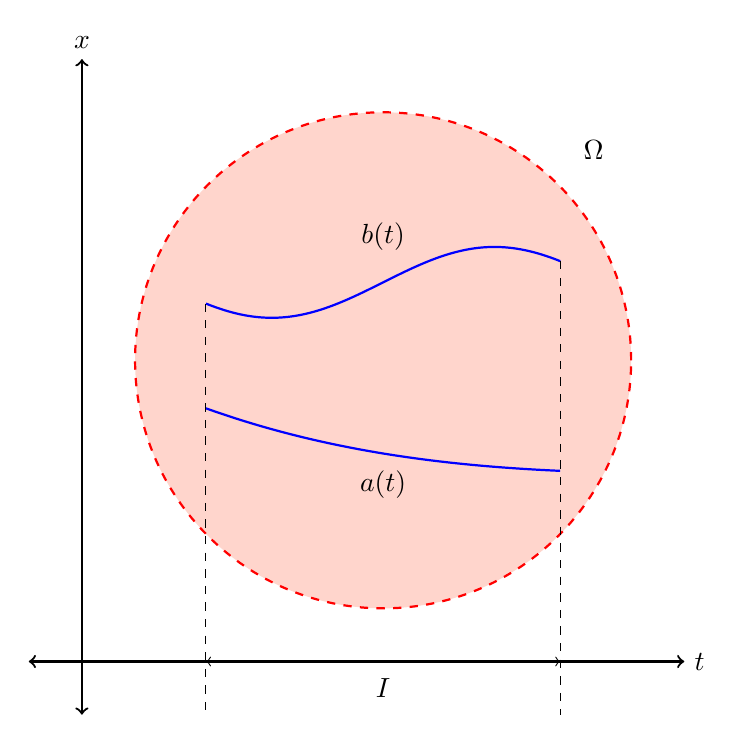
\begin{tikzpicture}[scale=0.9]
        \def\omgr{3.5}
        \def\omgm{0.75}
        \def\dom{-\omgr + 1: \omgr - 1}
        \def\b(#1){1.1+0.5 * sin((#1) r)}
        \def\a(#1){-(0.001*(#1-5.4)^2 +0.002*(#1-5.4)^3)-1.6}
        \filldraw[fill=Coral1!30, draw=red, dashed, thick] (0,0) circle (\omgr);
        \node at (\omgr * 1.2 * 0.7071, \omgr * 1.2 * 0.7071) {$\Omega$};
        \draw[blue, thick, domain=\dom, samples=100] plot (\x,{\b(\x)});
        \draw[blue, thick, domain=\dom, samples=100] plot (\x,{\a(\x)});
        \draw[<->, thick] (-\omgr - 2 *\omgm,-\omgm - \omgr) -- (\omgr + \omgm,-\omgm - \omgr) node[right] {$t$};
        \draw[<->, thick] (-\omgr - \omgm, -2 * \omgm - \omgr) -- (-\omgm - \omgr,\omgr + \omgm) node[above] {$x$};
        \node at (0, 0.5*\omgr) {$b(t)$};
        \node at (0, -0.5*\omgr) {$a(t)$};
        \draw[-, dashed, black] (-\omgr + 1, {\b(-\omgr + 1)}) -- (-\omgr + 1, -\omgr - 2*\omgm);
        \draw[-, dashed, black] (\omgr - 1, {\b(\omgr - 1)}) -- (\omgr - 1, -\omgr - 2*\omgm);
        \draw[<->, black] (-\omgr + 1, -\omgr - \omgm) -- (\omgr - 1, -\omgr - \omgm);
        \node at (0, -\omgr - 1.5*\omgm) {$I$};
    \end{tikzpicture}
\end{center}
Fijamos $t_0 \in I$ cualquiera. La función $F(t_0)$ ``recorre'' la variable $x$ integrando $f$ entre $a(t_0)$ y $b(t_0)$. Comencemos con la demostración.
\vspace{2mm} \newline \indent Sea $(t_n)_{n\in\N} \subseteq I \setminus \{t_0\}$ con $t_n \xrightarrow{n\to\infty} t_0$. Escribiremos la expresión de $F'(t_0)$ sin llegar todavía a tomar límites:
\begin{flalign*}
    &\frac{F(t_n) - F(t_0)}{t_n - t_0} = \frac{1}{t_n - t_0}\left(\int_{a(t_n)}^{b(t_n)}f(t_n, x)dx - \int_{a(t_0)}^{b(t_0)}f(t_0, x)dx\right) = \\[2ex]
    &\hspace{1mm} = \frac{1}{t_n - t_0} \left(\int_{a(t_n)}^{b(t_n)}f(t_n, x)dx - \int_{a(t_n)}^{b(t_0)}f(t_n, x)dx + \int_{a(t_n)}^{b(t_0)}f(t_n, x)dx - \right.\\[2ex]
    &\hspace{5ex} \left. - \int_{a(t_0)}^{b(t_0)}f(t_n, x)dx + \int_{a(t_0)}^{b(t_0)}f(t_n, x)dx - \int_{a(t_0)}^{b(t_0)}f(t_0, x)dx\right) = \\[2ex]
    &\hspace{1mm} = \frac{1}{t_n - t_0} \left(\int_{b(t_0)}^{b(t_n)}f(t_n,x)\,dx - \int_{a(t_0)}^{a(t_n)}f(t_n, x)\,dx - \int_{a(t_0)}^{b(t_0)}f(t_n,x)-f(t_0, x)\,dx\right) = (*)
\end{flalign*}
\vspace{2mm} Aplicando el Teorema del Valor Medio de Integración, existen $\xi_n \in I_{b(t_n), b(t_0)}$ y $\zeta_n \in I_{a(t_n), a(t_0)}$ tales que:
$$(*)= f(t_n, \xi_n) \cdot \frac{b(t_n)-b(t_0)}{t_n - t_0} - f(t_n, \zeta_n)\cdot \frac{a(t_n) - a(t_0)}{t_n - t_0} + \int_{a(t_0)}^{b(t_0)}\frac{f(t_n, x) - f(t_0, x)}{t_n - t_0} \,dx$$
\vspace{2mm} Por ser $a$  y $b$ derivables, tomando límites en los dos primeros sumandos:
$$\lim_{n\to\infty} f(t_n, \xi_n) \cdot \frac{b(t_n)-b(t_0)}{t_n - t_0} - f(t_n, \zeta_n)\cdot \frac{a(t_n) - a(t_0)}{t_n - t_0} = f\big(t_0, b(t_0)\big) \cdot b'(t_0) - f\big(t_0, a(t_0)\big) \cdot a'(t_0)$$
\vspace{2mm} Por el Teorema del Valor Medio de Derivación, sabemos que existe $\theta_n \in I_{t_n, t_0}$ tal que $\frac{f(t_n, x)- f(t_0, x)}{t_n - t_0} = \frac{\partial f}{\partial t}(\theta_n , x)$. Además, por ser $\Omega$ un abierto con $f$ continua en él, podemos afirmar que existen $\varepsilon > 0$, $\delta > 0$ tales que:
\begin{flalign*}
    &J := [t_0 - \delta, t_0 + \delta] \times [a(t_0) - \varepsilon, a(t_0) + \varepsilon] \subseteq \Omega \\
    &K := [t_0 - \delta, t_0 + \delta] \times [b(t_0) - \varepsilon, b(t_0) + \varepsilon] \subseteq \Omega
\end{flalign*}
Así, sea $t \in [t_0 - \delta, t_0 + \delta]$, tenemos que $a(t) \in [a(t_0) - \varepsilon, a(t_0) + \varepsilon]$ y $b(t) \in [b(t_0) - \varepsilon, b(t_0) + \varepsilon]$. Definimos $M := [t_0 - \delta, t_0 + \delta] \times [a(t_0) - \varepsilon, b_(t_0) + \varepsilon]$. Veamos qué papel juegan estos conjuntos en nuestro esquema anterior:
\vspace{6mm} \newline
\begin{minipage}{0.5\textwidth}
    \begin{center}
        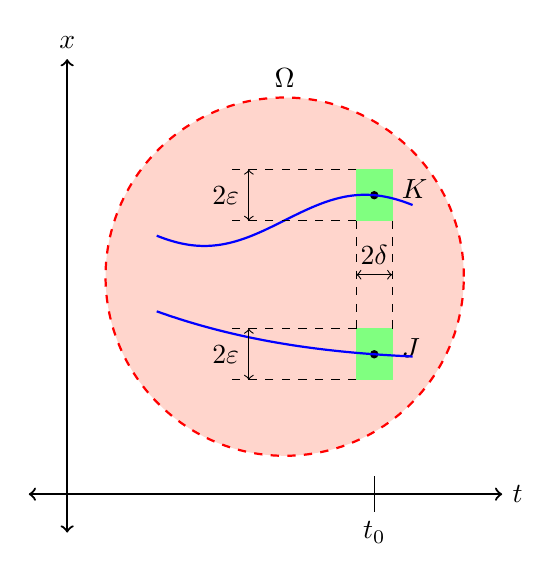
\begin{tikzpicture}[scale=0.65]
            \def\omgr{3.5}
            \def\omgm{0.75}
            \def\dom{-\omgr + 1: \omgr - 1}
            \def\t0{0.5*\omgr}
            \def\eps{0.5}
            \def\delt{0.35}
            \def\b(#1){1.1+0.5 * sin((#1) r)}
            \def\a(#1){-(0.001*(#1-5.4)^2 +0.002*(#1-5.4)^3)-1.6}
            \draw[<->, thick] (-\omgr - 2 *\omgm,-\omgm - \omgr) -- (\omgr + \omgm,-\omgm - \omgr) node[right] {$t$};
            \draw[<->, thick] (-\omgr - \omgm, -2 * \omgm - \omgr) -- (-\omgm - \omgr,\omgr + \omgm) node[above] {$x$};
            \filldraw[fill=Coral1!30, draw=red, dashed, thick] (0,0) circle (\omgr);
            \node[above, text=black] at (0, \omgr) {$\Omega$};        
            \filldraw[green!50] ({\t0 - \delt}, {\b(\t0) - \eps}) rectangle ({\t0 + \delt}, {\b(\t0) + \eps}) node[anchor=north west] {$\textcolor{black}{K}$};
            \filldraw[green!50] ({\t0 - \delt}, {\a(\t0) - \eps}) rectangle ({\t0 + \delt}, {\a(\t0) + \eps}) node[anchor=north west] {$\textcolor{black}{J}$};
            \filldraw[black] ({\t0}, {\b(\t0)}) circle (2pt);
            \filldraw[black] ({\t0}, {\a(\t0)}) circle (2pt);
            \draw[blue, thick, domain=\dom, samples=100] plot (\x,{\b(\x)});
            \draw[blue, thick, domain=\dom, samples=100] plot (\x,{\a(\x)});
            \draw[dashed] ({\t0 + \delt}, {\b(\t0) - \eps}) -- ({\t0 + \delt}, {\a(\t0) + \eps});
            \draw[dashed] ({\t0 - \delt}, {\b(\t0) - \eps}) -- ({\t0 - \delt}, {\a(\t0) + \eps});
            \draw[<->] ({\t0 - \delt},{0.5*(\b(\t0) + \a(\t0))}) -- ({\t0 + \delt},{0.5*(\b(\t0) + \a(\t0))}) node[midway,above] {$2\delta$};
            \draw[dashed] ({\t0 - \delt}, {\b(\t0) - \eps}) -- ({\t0 - 8*\delt}, {\b(\t0) - \eps});
            \draw[dashed] ({\t0 - \delt}, {\b(\t0) + \eps}) -- ({\t0 - 8*\delt}, {\b(\t0) + \eps});
            \draw[<->] ({\t0 - 7* \delt},{\b(\t0) + \eps}) -- ({\t0 - 7 *\delt},{\b(\t0) - \eps}) node[midway,left] {$2\varepsilon$};
            \draw[dashed] ({\t0 - \delt}, {\a(\t0) - \eps}) -- ({\t0 - 8*\delt}, {\a(\t0) - \eps});
            \draw[dashed] ({\t0 - \delt}, {\a(\t0) + \eps}) -- ({\t0 - 8*\delt}, {\a(\t0) + \eps});
            \draw[<->] ({\t0 - 7* \delt},{\a(\t0) + \eps}) -- ({\t0 - 7 *\delt},{\a(\t0) - \eps}) node[midway,left] {$2\varepsilon$};
            \draw[-] (\t0, -\omgr - \omgm + \delt) -- (\t0, -\omgr - \omgm - \delt) node[below] {$t_0$};
        \end{tikzpicture}
    \end{center}
\end{minipage}
\begin{minipage}{0.5\textwidth}    
    \begin{center}
    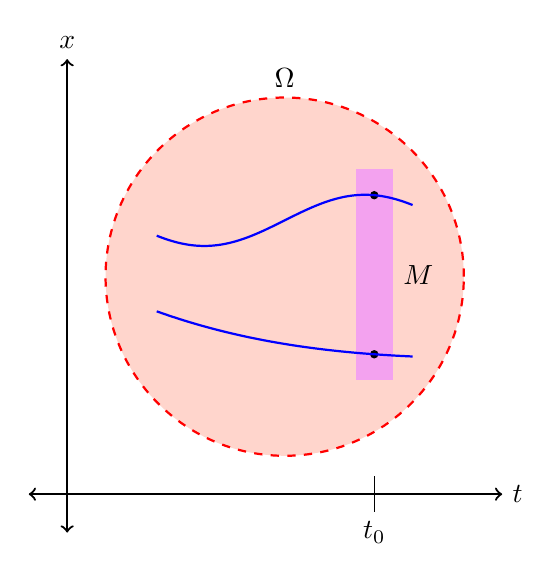
\begin{tikzpicture}[scale=0.65]
        \def\omgr{3.5}
        \def\omgm{0.75}
        \def\dom{-\omgr + 1: \omgr - 1}
        \def\t0{0.5*\omgr}
        \def\eps{0.5}
        \def\delt{0.35}
        \def\b(#1){1.1+0.5 * sin((#1) r)}
        \def\a(#1){-(0.001*(#1-5.4)^2 +0.002*(#1-5.4)^3)-1.6}
        \draw[<->, thick] (-\omgr - 2 *\omgm,-\omgm - \omgr) -- (\omgr + \omgm,-\omgm - \omgr) node[right] {$t$};
        \draw[<->, thick] (-\omgr - \omgm, -2 * \omgm - \omgr) -- (-\omgm - \omgr,\omgr + \omgm) node[above] {$x$};
        \filldraw[fill=Coral1!30, draw=red, dashed, thick] (0,0) circle (\omgr);
        \node[above, text=black] at (0, \omgr) {$\Omega$};        
        \filldraw[Orchid2!70] ({\t0 - \delt}, {\a(\t0) - \eps}) rectangle ({\t0 + \delt}, {\b(\t0) + \eps}) node[midway, right, xshift={20*\delt}] {$\textcolor{black}{M}$};
        \filldraw[black] ({\t0}, {\b(\t0)}) circle (2pt);
        \filldraw[black] ({\t0}, {\a(\t0)}) circle (2pt);
        \draw[blue, thick, domain=\dom, samples=100] plot (\x,{\b(\x)});
        \draw[blue, thick, domain=\dom, samples=100] plot (\x,{\a(\x)});       
        \draw[-] (\t0, -\omgr - \omgm + \delt) -- (\t0, -\omgr - \omgm - \delt) node[below] {$t_0$};
    \end{tikzpicture}
    \end{center}
\end{minipage}
\vspace{6mm} \newline \indent Tenemos que $M$ es compacto por definición. Además, como $f \in \mathcal{C}^1(\Omega)$ por hipótesis, podemos garantizar que:
$$\exists \hspace{1mm} m := \max \left\{\left|\frac{\partial f}{\partial t}(x, t)\right| : (x,t) \in M\right\} $$
De este modo, estamos en condiciones de aplicar el \hyperref[result:2.2.7]{Teorema de la Convergencia Dominada}. Por todo lo anterior,
\begin{flalign*}
    \lim_{n\to\infty}& f(t_n, \xi_n) \cdot \frac{b(t_n)-b(t_0)}{t_n - t_0} - f(t_n, \zeta_n)\cdot \frac{a(t_n) - a(t_0)}{t_n - t_0} + \int_{a(t_0)}^{b(t_0)}\frac{f(t_n, x) - f(t_0, x)}{t_n - t_0}\,dx = \\[2ex]
    &= f\big(t_0, b(t_0)\big) \cdot b'(t_0) - f\big(t_0, a(t_0)\big) \cdot a'(t_0) + \int_{a(t_0)}^{b(t_0)} \frac{\partial f}{\partial t}(x, t_0) \,dx
\end{flalign*}

\newpage
\chapter{Cálculo de la integral de Lebesgue en \texorpdfstring{$\R^N$}{R\^N}}
\result{Notación y conceptos iniciales}
\hspace{3mm} $\R^{p+q} = \R^p \times \R^q$ con $p,q\in\N$. Así, si $x \in \R^p$ con $y \in \R^q$; entonces, $(x,y) \in \R^{p+q}$.
\newline \indent Sea $E \subseteq \R^{p+q}$, sea $x \in \R^p$. Definimos la sección de $E$ por $x$ como el conjunto:
$$E_x = \Big\{y \in \R^q : (x,y) \in E\Big\}$$
De manera similar, sea $y \in \R^{q}$, definimos la sección de $E$ por $y$ como:
$$E_y = \Big\{x \in \R^p : (x,y) \in E\Big\}$$
\indent Sea $f: \R^{p+q} \longrightarrow \overline{\R}$ \hspace{1mm} $(x,y) \longmapsto f(x,y)$. Definimos la sección de $f$ por $x \in \R^p$ y la sección de $f$ por $y \in \R^q$ (respectivamente) como las dos siguientes funciones: \\[-2.5ex]
\begin{minipage}{0.5\textwidth}
    \begin{flalign*}
        f_x :& \R^q \longrightarrow \overline{\R}\\
        &y \longmapsto f(x,y)
    \end{flalign*}
\end{minipage}
\begin{minipage}{0.5\textwidth}
    \begin{flalign*}
        f_y :& \R^p \longrightarrow \overline{\R}\\
        &x \longmapsto f(x,y)
    \end{flalign*}
\end{minipage}

\vspace{6mm} \result{Propiedades de las secciones}
\hspace{3mm} Sea $f : \R{p+q} \longrightarrow \overline{\R}$. Sean $\{E\}\cup\{E^i\}_{i\in\N} \subseteq \R^{p+q}$. Sean $x \in \R^p, y \in \R^q$. Entonces, se cumplen los siguientes enunciados:
\\[2ex]
\begin{minipage}{0.5\textwidth}
    \begin{enumerate}[label=\roman*)]
        \item $(f^+)_x = (f_x)^+$
        \item $(f^-)_x = (f_x)^-$
        \item $(\smallcup_{i\in\N}E^i)_x = \smallcup_{i\in\N}E^i_x$
        \item $(\smallcap_{i\in\N}E^i)_x = \smallcap_{i\in\N}E^i_x$
        \item $(\R^{p+q}\setminus E)_x = \R^q \setminus E_x$.
    \end{enumerate}
\end{minipage}
\begin{minipage}{0.5\textwidth}
    \begin{enumerate}[label=\roman*')]
        \item $(f^+)_y = (f_y)^+$
        \item $(f^-)_y = (f_y)^-$
        \item $(\smallcup_{i\in\N}E^i)_y = \smallcup_{i\in\N}E^i_y$
        \item $(\smallcap_{i\in\N}E^i)_y = \smallcap_{i\in\N}E^i_y$
        \item $(\R^{p+q}\setminus E)_y = \R^p \setminus E_y$.
    \end{enumerate}
\end{minipage}
\\[4ex] \dem Las demostraciones $(*')$ son análogas al resto.
\vspace{2mm} \newline $\romannumeral 1)$ $(f_x)^+(y) = \max\{f_x(y),0\} = \max\{f(x,y), 0\} = f^+(x,y) = (f^+)_x(y)$.
\vspace{2mm} \newline $\romannumeral 2)$ $(f_x)^-(y) = \max\{-f_x(y),0\} = \max\{-f(x,y), 0\} = f^-(x,y) = (f^-)_x(y)$.
\vspace{6mm} \newline $\romannumeral 3)$ Veamos que $(\smallcup_{i\in\N}E^i)_y = \smallcup_{i\in\N}E^i_y$ por doble contenido:
\begin{tcolorbox}[Subset-contingency]
    $\subseteq$ \hspace{2mm} Si $y \in (\smallcup_{i\in\N}E^i)_x$, tenemos $(x,y) \in \smallcup_{i\in\N}E^n$ luego $\exists \hspace{1mm} j \in \N$ tal que $(x,y) \in E_j$. 
\end{tcolorbox}
Por tanto, $y \in E^j_x \subseteq \smallcup_{i\in\N}E^i_x$.
\vspace{2mm}
\begin{tcolorbox}[Subset-contingency]
    $\supseteq$ \hspace{2mm} Si $y \in \smallcup_{i\in\N}E^i_x$, tenemos $\exists \hspace{1mm} j \in \N$ tal que $y \in E^j_x$. Así, $(x,y) \in E^j \subseteq \smallcup_{i\in\N} E^i$.
\end{tcolorbox}
Por tanto, $y \in (\smallcup_{i\in\N} E^i)_x$.

\vspace{8mm} $\romannumeral 4)$ Lo veremos por la definición del conjunto. Como $y$ es un punto fijo de $\R^q$ (dado por el enunciado), usaremos $z$ como variable genérica de $\R^q$.
\begin{flalign*}
    (\smallcap_{i\in\N}E^i)_x = \Big\{z \in \R^q : (x,z) \in \smallcap_{i\in\N}E^i\Big\} = \bigcap_{i\in\N}\Big\{z \in \R^q : (x,z) \in E^i\Big\} = \smallcap_{i\in\N}E^i_x
\end{flalign*}

\vspace{8mm} \noindent $\romannumeral 5)$ Veamos que $(\R^{p+q}\setminus E)_x = \R^q \setminus E_x$ por doble contenido:
\begin{tcolorbox}[Subset-contingency]
    $\subseteq$ \hspace{2mm} Si $y \in (\R^{p+q}\setminus E)_x$, tenemos $(x,y) \in \R^{p+q} \setminus E$ luego $(x,y) \notin E$. 
\end{tcolorbox}
Por tanto, $y \notin \{z \in \R^q : (x,z) \in E\} = E_x$ luego $y \in \R^q \setminus E_x$.
\vspace{2mm}
\begin{tcolorbox}[Subset-contingency]
    $\subseteq$ \hspace{2mm} Si $y \in \R^{q}\setminus E_x$, tenemos $y \notin \{z \in \R^q : (x,y) \in E\} = E_x$. 
\end{tcolorbox}
Por tanto, $(x,y) \notin E$ luego $(x,y) \in \R^{p+q} \setminus E$ y por tanto $y \in (\R^{p+q} \setminus E)_x$.

\vspace{6mm} \noindent $\nota$ A partir de los apartados $(iii)$, $(iv)$, $(iii')$ y $(iv')$ se deducen los siguientes para $E, F \in \R^{p+q}$ cualesquiera:
\begin{align*}
    v) \hspace{2mm}(E \setminus F)_x = E_x \setminus F_x &&
    v') \hspace{2mm}  (E \setminus F)_y = E_y \setminus F_y
\end{align*}

\newpage
\result{Teorema de anomalías de conjuntos medibles}
\hspace{3mm} Sea $E \in \mathfrak{M}_{p+q}$. Se cumplen los siguientes enunciados: \\[4ex]
\begin{minipage}{0.5\textwidth}
    \begin{enumerate}[leftmargin=0mm, label=\alph*)]
        \item $\exists \hspace{1mm} A \in \mathfrak{M}_p$ con $\mu_p(A) = 0$ que verifica: \\[-3ex]
        $$\forall \hspace{1mm} x \in \R^p \setminus A : E_x \in \mathfrak{M}_q$$
        \item La siguiente función es $\mu_p$-medible: \\[-6ex]
        \begin{align*}
            \varphi : \R^p \setminus A \to \R&& x \mapsto \varphi(x) = \mu_q(E_x)
        \end{align*}
        \item Medida por secciones en $x$: \\[-2ex]
        $$\int_{\R^p \setminus A}\varphi(x)\,d\mu_p(x) = \mu_{p+q}(E)$$
    \end{enumerate}
\end{minipage}
\begin{minipage}{0.5\textwidth}
    \begin{enumerate}[leftmargin=7mm, rightmargin=0mm, label=\alph*')]
        \item $\exists \hspace{1mm} B \in \mathfrak{M}_q$ con $\mu_p(A) = 0$ que verifica: \\[-3ex]
        $$\forall \hspace{1mm} y \in \R^q \setminus B : E_y \in \mathfrak{M}_p$$
        \item La siguiente función es $\mu_q$-medible: \\[-6ex]
        \begin{align*}
            \psi : \R^q \setminus B \to \R&& y \mapsto \psi(y) = \mu_p(E_y)
        \end{align*}
        \item Medida por secciones en $y$: \\[-2ex]
        $$\int_{\R^q \setminus B}\psi(y)\,d\mu_q(y) = \mu_{p+q}(E)$$
    \end{enumerate}
\end{minipage}
\\[6ex] \dem Veremos solo los tres primeros apartados (los apartados' son análogos). Iremos estructurando la demostración por casos de complejidad incremental.

\vspace{6mm} $\romannumeral 1)$ Para $E$ un cubo acotado. Podemos expresar $E = I \times J$ con $I, J$ cubos acotados de $\R^p$ y $\R^q$, respectivamente.
\begin{adjustwidth}{0.07\textwidth}{}
    \vspace{-3ex}
    \begin{flalign*}
        \text{a) Sea } x\in\R^p, E_x = \begin{cases}
            J &\text{si } x \in I \\
            \varnothing &\text{si } x \notin I
        \end{cases} \hspace{4mm} \text{ En cualquier caso, }E_x \in \mathfrak{M}_q&&
    \end{flalign*}
    \\[-3ex]
    \begin{flalign*}
        \text{b) }\varphi(x) = \left.\begin{cases}
        \mu_q(J) &\text{ si } x \in I\\
        \mu_q(\varnothing) &\text{ si } x \notin I
        \end{cases}\right\} = \mu_q(J) \cdot X_I(x) \hspace{2mm} \text{ que es } \mu_p\text{-medible}.&&
    \end{flalign*}
    \begin{flalign*}
        \text{c) } \int_{\R^p}\varphi(x)\,d\mu_p(x) = \mu_q(J) \cdot \int_{\R^p}X_I(x)\,d\mu_p(x) = \mu_p(I) \cdot \mu_q(J) = \mu_{p+q}(E)&&
    \end{flalign*}
\end{adjustwidth}

\vspace{6mm} $\romannumeral 2)$ Para $E$ un abierto acotado. Sabemos que podemos expresar $E = \smallcup_{n\in\N}I^n$ donde los $I_n$ son cubos diádicos disjuntos. Aplicando el apartado anterior a cada uno de ellos, sabemos que para $x \in \R^p$ cualquiera, se tiene:
\\[-3ex]  %TODO referenciar resultado cubos diádicos
\begin{align*}
    I^n_x \in \mathfrak{M}_q &&
    \varphi_n(x) = \mu_q(I_x^n) \hspace{2mm} \mu_p\text{-medible} &&
    \int_{\R^p}\varphi_n(x)\,d\mu_p(x) = \mu_{p+q}(I^n)
\end{align*}
Veamos cómo demostrar el apartado $(\romannumeral 2)$ en base a esta información:
\begin{adjustwidth}{0.07\textwidth}{}
    \vspace{-5ex}
    \begin{flalign*}
        \text{a) }E_x = (\smallcup_{n\in\N}I^n)_x \overset{\hyperref[result:2.4.2]{2.4.2}}{=} \smallcup_{n\in\N} I^n_x \in \mathfrak{M}_q \hspace{4ex} \text{ Consideramos } A = \varnothing.&&
    \end{flalign*}
    \\[-8ex]
    \begin{flalign*}
        %TODO referenciar resultado de límite medible
        \text{b) }\varphi(x) = \mu_q(E_x) =\mu_q \big(\smallcup_{n\in\N}I^n_x\big)  =\sum_{n=1}^{\infty}\mu_q(I^n_x) = \lim_{n\to \infty} \sum_{k=1}^{n}\varphi_k(x) \hspace{2ex} \mu_q\text{-medible}.&&
    \end{flalign*}
    \\[-6ex]
    \begin{flalign*}
        \text{c) }& \int_{\R^p}\varphi(x)\,d\mu_p(x) = \int_{\R^p}\sum_{n=1}^{^\infty}\varphi_n(x)\,d\mu_p(x) \overset{\hyperref[result:2.1.10]{TCM}}{=} \sum_{n=1}^{\infty} \int_{\R^p}\varphi_n\,d\mu_p(x) =&& \\
        &= \sum_{n=1}^{\infty} \mu_{p+q}(I^n) = \mu_{p+q}\big(\smallcup_{n\in\N}I^n\big) = \mu_{p+q}(E)
    \end{flalign*}
\end{adjustwidth}

\vspace{6mm} $\romannumeral 3)$ Para $E = \smallcap_{n\in\N}O^n$ intersección de abiertos decrecientes. Aplicando el apartado anterior, sabemos que para $x \in \R^p$ cualquiera se cumple:
\begin{align*}
    O^n_x \in \mathfrak{M}_q &&
    \varphi_n(x) = \mu_q(O_x^n) \hspace{2mm} \mu_p\text{-medible} &&
    \int_{\R^p}\varphi_n(x)\,d\mu_p(x) = \mu_{p+q}(O^n)
\end{align*}
Demostraremos el apartado $(\romannumeral 3)$ con esta información:
\begin{adjustwidth}{0.07\textwidth}{}
    \vspace{-5ex}
    \begin{flalign*}
        \text{a) }E_x = (\smallcap_{n\in\N}O^n)_x \overset{\hyperref[result:2.4.2]{2.4.2}}{=} \smallcap_{n\in\N} O^n_x \in \mathfrak{M}_q \hspace{4ex} \text{ Consideramos } A = \varnothing.&&
    \end{flalign*}
    \\[-8ex]
    \begin{flalign*}
        %TODO referenciar resultado de límite por abajo de la medida
        \text{b) }\varphi(x) = \mu_q(E_x) =\mu_q \big(\smallcap_{n\in\N}O^n_x\big)  = \lim_{n\to\infty}\mu_q(O^n_x) = \lim_{n\to\infty}\varphi_n(x) \hspace{4mm} \mu_q\text{-medible}&&
    \end{flalign*}
    \\[-6ex]
    \begin{flalign*}
        \text{c) }& \int_{\R^p}\varphi(x)\,d\mu_p(x) = \int_{\R^p}\lim_{n\to\infty}\varphi_n(x)\,d\mu_p(x) \overset{\hyperref[result:2.2.7]{TCD \hspace{1mm}\varphi_1}}{=} \lim_{n\to\infty} \int_{\R^p}\varphi_n\,d\mu_p(x) =&& \\
        &= \lim_{n\to\infty}\mu_{p+q}(O^n) = \mu_{p+q}(E)
    \end{flalign*}
\end{adjustwidth}

%TODO referenciar
\vspace{6mm} $\romannumeral 4) \hspace{2mm} E \in \mathfrak{M}_{p+q}$ con $\mu_{p+q}(E) = 0$. Por la caracterización topológica de los conjuntos medibles, sabemos que existen $\{O^n\}_{n\in\N} \subseteq \tau_{\R^{p+q}}$ con $E \subseteq O^{n+1} \subseteq O^n$ y tales que $\mu_{p+q}(O^n) \xrightarrow{n\to\infty}0$. De este modo, tenemos $E \subseteq N:= \smallcap_{n\in\N}O^n \in \mathfrak{M}_{p+q}$. Aplicando el apartado anterior a $N$, tenemos que para $x\in\R^p$ se cumple:
\vspace{-1.5ex}
\begin{align*}
    N_x \in \mathfrak{M}_q &&
    \varphi_1(x) = \mu_q(N_x) \hspace{2mm} \mu_p\text{-medible} &&
    \int_{\R^p}\varphi_1(x)\,d\mu_p(x) = \mu_{p+q}(N) = 0
\end{align*}

%TODO referenciar integral nula de función no negativa
\vspace{-1.5ex} \noindent Al ser $\varphi_1$ no negativa con integral nula, sabemos que $\varphi_1 \overset{\mu-a.e.}{=} 0$ luego $\exists \hspace{1mm} A \in \mathfrak{M}_p$ con $\mu_p(A) = 0$ tal que $\{x \in \R^p : \varphi_1(x) \neq 0\} \subseteq A$. Sea este el conjunto de anomalías para este apartado, dado $x \in \R^p \setminus A$, se cumple:
\begin{adjustwidth}{0.07\textwidth}{}
    \vspace{-5ex}
    \begin{flalign*}
        \text{a) }E_x \subseteq N_x \text{ con } \mu_q(E_x) \leq \mu_q(N_x) = \varphi_1(x) = 0 \text{ luego } E_x \in \mathfrak{M}_q.&&
    \end{flalign*}
    \\[-10ex]
    \begin{flalign*}
        \text{b) }\varphi(x) = \mu_q(E_x) =0 \hspace{4mm} \mu_q\text{-medible trivialmente}.&&
    \end{flalign*}
    \\[-9ex]
    \begin{flalign*}
        \text{c) }& \int_{\R^p \setminus A}\varphi(x)\,d\mu_p(x) = \int_{\R^p \setminus A}0\,d\mu_p(x) = 0 = \mu_{p+q}(E)&&
    \end{flalign*}
\end{adjustwidth}

%TODO referenciar expresión de medibles Lebesgue según borelianos
\vspace{6mm} $\romannumeral 5)$ Para $E \in \mathfrak{M}_{p+q}$ acotado. Por ser medible, $E = G\setminus N$, donde $G$ es una intersección de abiertos decrecientes y $N$ es un conjunto de medida nula. Al ser $E$ acotado, también ha de serlo $G$, luego estamos en condiciones de aplicarle el apartado $(\romannumeral 3)$. Así, para $x \in \R^p$ se cumple:
\vspace{-2ex}
\begin{align*}
    G_x \in \mathfrak{M}_q &&
    \varphi_1(x) = \mu_q(G_x) \hspace{2mm} \mu_p\text{-medible} &&
    \int_{\R^p}\varphi_1(x)\,d\mu_p(x) = \mu_{p+q}(G)
\end{align*}

\vspace{-1.5ex} \noindent Aplicando ahora el apartado $(\romannumeral 4)$ a $N$, para $x \in \R^p \setminus A$ se tiene:
\vspace{-1ex}
\begin{align*}
    N_x \in \mathfrak{M}_q &&
    \varphi_2(x) = \mu_q(N_x) \hspace{2mm} \mu_p\text{-medible} &&
    \int_{\R^p \setminus A}\varphi_2(x)\,d\mu_p(x) = \mu_{p+q}(N)
\end{align*}

\vspace{-1.5ex} \noindent Consideramos este conjunto $A$. Así, dado $x \in \R^p \setminus A$, tenemos:
\begin{adjustwidth}{0.07\textwidth}{}
    \vspace{-5ex}
    \begin{flalign*}
        \text{a) }E_x \subseteq N_x \text{ con } \mu_q(E_x) \leq \mu_q(N_x) = \varphi_1(x) = 0 \text{ luego } E_x \in \mathfrak{M}_q.&&
    \end{flalign*}
    \\[-10ex]
    \begin{flalign*}
        \text{b) }\varphi(x) = \mu_q(E_x) = \mu_q(G_x) - \mu_q(N_x) = \varphi_1(x) - \varphi_2(x) \hspace{4mm} \mu_q\text{-medible}.&&
    \end{flalign*}
    \\[-8ex]
    \begin{flalign*}
        \text{c) }& \int_{\R^p \setminus A}\varphi(x)\,d\mu_p(x) = \int_{\R^p \setminus A}0\,d\mu_p(x) = 0 = \mu_{p+q}(E)&&
    \end{flalign*}
\end{adjustwidth}

%TODO referenciar conjuntos medibles según borelianos
\vspace{6mm} $\romannumeral 6)$ $E \in \mathfrak{M}_{p+q}$ (caso general). Definimos $E^n = E \cap [-n,n]^N$. De este modo, es claro que $E = \smallcup_{n\in\N}E^n$ y que todos los $E^n$ son acotados. Aplicando el apartado ($\romannumeral 5$) a cada uno de ellos, tenemos que para $x \in \R^p \setminus A^n$ se cumple:
\begin{align*}
    E^n_x \in \mathfrak{M}_q &&
    \varphi_n(x) = \mu_q(E^n_x) \hspace{2mm} \mu_p\text{-medible} &&
    \int_{\R^p \setminus A^n}\varphi_1(x)\,d\mu_p(x) = \mu_{p+q}(E^n)
\end{align*}
Consideramos el conjunto de anomalías $A := \smallcup_{n\in\N} A^n$ aplicando la subaditividad de la medida, es claro que $\mu_{p+q}(A) = 0$. Sea $x \in R^p \setminus A$, se cumple:
\begin{adjustwidth}{0.07\textwidth}{}
    \vspace{-5ex}
    \begin{flalign*}
        \text{a) }E_x = \smallcup_{i\in\N}\underbracket{E^n_x}_{\in \mathfrak{M}_q} \in \mathfrak{M}_q &&
    \end{flalign*}
    \\[-10ex]
    \begin{flalign*}
        \text{b) }\varphi(x) = \mu_q(E_x) =  \lim_{n\to\infty}\mu_q(E^n_x) = \lim_{n\to\infty}\varphi_n(x)\hspace{4mm} \mu_q\text{-medible}.&&
    \end{flalign*}
    \\[-9ex]
    \begin{flalign*}
        \text{c) }& \int_{\R^p \setminus A}\varphi(x)\,d\mu_p(x) = \int_{\R^p \setminus A} \lim_{n\to\infty}\varphi_n(x)\,d\mu_p(x) \overset{\hyperref[result:2.1.10]{TCM}}{=} \lim_{n\to\infty} \int_{R^p \setminus A}\varphi_n(x)\,d\mu = &&\\[2ex]
         &= \lim_{n \to \infty} \mu_{p+q}(E^n) = \mu_{p+q}(E)
    \end{flalign*}
\end{adjustwidth}

\vspace{6mm}
\result{Teorema de Tonelli}
\hspace{3mm} Sea $f : \R^{p+q} \longrightarrow [0,+\infty]$ una función $\mu_{p+q}$-medible. Tenemos:
\\[3ex]
\begin{minipage}{0.5\textwidth}
    \begin{enumerate}[leftmargin=0mm, label=\alph*)]
        \item $\exists A \in \mathfrak{M}_q$ con $\mu_p(A)=0$ que verifica: \\[-3ex] 
        $$\forall \hspace{1mm} x \in \R^p \setminus A \hspace{1mm} f_x \text{ es } \mu_q\text{-medible}$$
        \item La siguiente función $\varphi : \R^p \setminus A \to [0,+\infty]$ \\[-6ex]
        \begin{align*}
            x \mapsto \int_{\R^q}f_x(y)\,d\mu_q(y) && \text{ es }\mu_q\text{-medible}
        \end{align*}
        \item Integración por secciones: \\[-2.5ex]
        $$\hspace{-5ex} \int_{\R^p \setminus A} \hspace{-3mm} \varphi(x)\,d\mu_p(x) = \int_{\R^{p+q}} \hspace{-3mm} f(x,y)\,d\mu_{p+q}(x,y)$$
    \end{enumerate}
\end{minipage}
\begin{minipage}{0.55\textwidth}
    \begin{enumerate}[leftmargin=8mm, rightmargin=-2mm, label=\alph*')]
        \item $\exists B \in \mathfrak{M}_p$ con $\mu_p(B)=0$ que verifica: \\[-3ex] 
        $$\forall \hspace{1mm} y \in \R^q \setminus B \hspace{1mm} f_y \text{ es } \mu_p\text{-medible}$$
        \item La siguiente función $\psi : \R^q \setminus B \to [0,+\infty]$ \\[-6ex]
        \begin{align*}
            y \mapsto \int_{\R^p}f_y(x)\,d\mu_p(x) && \text{ es }\mu_p\text{-medible}
        \end{align*}
        \item Integración por secciones: \\[-2.5ex]
        $$\int_{\R^q \setminus B} \hspace{-3mm} \varphi(y)\,d\mu_q(y) = \int_{\R^{p+q}} \hspace{-3mm} f(x,y)\,d\mu_{p+q}(x,y)$$
    \end{enumerate}
\end{minipage}
Por tanto, ha de cumplirse:
$$ \int_{\R^p}\left(\int_{\R^q}f(x,y)\,d\mu_q(y)\right)\,d\mu_p(x) = \int_{\R^{p+q}} \hspace{-4mm} f(x,y)\,d\mu_{p+q}(x,y) = \int_{\R^q}\left(\int_{\R^p}f(x,y)\,d\mu_p(x)\right)\,d\mu_q(y)$$

\vspace{2mm} \dem Al igual que con el caso anterior; dividiremos la demostración en casos, y no se demostrarán los apartados' al ser análogos.
\vspace{2mm} \newline $\romannumeral 1)$ Consideramos $f = X_E$ para cierto $E \in \mathfrak{M}_{p+q}$. Se corresponde con el \hyperref[result:2.4.3]{teorema anterior}. Así, para el correspondiente conjunto de anomalías $A \in \mathfrak{M}_{p+q}$ con $\mu_{p+q}(A) = 0$ fijado, tenemos:
\begin{adjustwidth}{0.07\textwidth}{}
    \vspace{-4ex}
    \begin{flalign*}
        \text{a) }f_x = (X_E)_x = X_{E_x} \mu_q\text{-medible al ser }E_x \in \mathfrak{M}_q&&
    \end{flalign*}
    \\[-8ex]
    \begin{flalign*}
        \text{b) }\varphi(x) = \int_{\R^q}X_{E_x}(y)\,d\mu_q(y) = \mu_q(E_x) \text{ medible por el \hyperref[result:2.4.3]{teorema anterior}}&&
    \end{flalign*}
    \\[-8ex]
    \begin{flalign*}
        \text{c) }\int_{\R^p \setminus A}\varphi(x)\,d\mu_p(x) = \mu_{p+q}(E) = \int_{\R^{p+q}}\underbrace{X_{E}(x,y)}_{f(x,y)}\,d\mu_{p+q}(x,y) &&
    \end{flalign*}
\end{adjustwidth}

\vspace{6mm} \indent $\romannumeral 2)$ Sea $f = \displaystyle \sum_{i=1}^{k} \lambda_i \cdot X_{E^i}$ función simple y medible dada por su expresión canónica. Aplicando el apartado anterior a cada $E^i$, tenemos que $\exists \hspace{1mm} A_i \in \mathfrak{M}_{p+q}$ con $\mu_{p+q}(A_i) = 0$ tal que $\forall \hspace{1mm} x \in \R^p \setminus A_i$ se cumple:
\begin{align*}
    (X_{E^i})_x \hspace{1mm} \mu_q\text{-medible} &&
    \varphi_i(x) = \int_{\R^q}X_{E^i_x}(y)\,d\mu_q(y) \text{ es }\mu_q\text{-medible}
\end{align*}
$$\int_{\R^p \setminus A_i}\varphi_i(x)\,d\mu_p(x) = \int_{\R^{p+q}}X_{E^i}(x,y)\,d\mu_{p+q}(x,y)$$

\vspace{4mm} Consideramos $A = \smallcup_{i\in\N}A_i \in \mathfrak{M}_{p}$, que cumple $\mu_p(A) = 0$ por subaditividad. Así, dado $x \in \R^p \setminus A$, se cumple:
\vspace{-5ex}
\begin{adjustwidth}{0.07\textwidth}{}
    \begin{flalign*}
        \text{a) } f_x = \sum_{i=1}^{k} \lambda_i \cdot \underbracket{X_{E^i}}_{\mu_q\text{-medible}} \hspace{1mm} \mu_q \text{-medible}&&
    \end{flalign*}
    \\[-6ex]
    \begin{flalign*}
        \text{b) } \varphi(x)& = \int_{\R^q}\sum_{i=1}^{k}\lambda_i \cdot X_{E^i_x}(y)\,d\mu_q(y)  = \sum_{i=1}^{k}\lambda_i \cdot \left(\int_{\R^q}X_{E^i_x}(y)\,d\mu_q(y)\right) =&& \\[1ex]
        &= \sum_{i=1}^k \lambda_i \cdot \underbracket{\varphi_i(x)}_{\mu_p \text{-medible}} \hspace{2mm} \mu_p \text{-medible}
    \end{flalign*}
    \\[-6ex]
    \begin{flalign*}
        \text{c) } \int_{\R^p \setminus A}&\varphi(x)\,d\mu_p(x) = \sum_{i=1}^{k} \lambda_i \cdot \int_{\R^p \setminus A}\varphi_i(x)\,d\mu_p(x) = \sum_{i=1}^{k}\lambda_i \cdot \int_{\R^p \setminus A_i}\varphi_i(x)\,d\mu_p(x) =&&\\
        =& \sum_{i=1}^k \lambda_i \cdot \mu_{p+q}(E^i) = \int_{\R^{p+q}}f(x,y)\,d\mu_{p+q}(x,y)
    \end{flalign*}
\end{adjustwidth}

%TODO referenciar funciones medibles como límite de simples
\vspace{6mm} $\romannumeral 3)$ $f \mu_{p+q}$-medible (caso general). Sabemos que existe una sucesión de funciones medibles y simples $(s_n)_{n\in\N}$ tales que $0\leq s_n \leq s_{n+1} \leq f$ que converge puntualmente a $f$. Aplicando el apartado anterior a cada $s_n$, tenemos que $\exists A_n \in \mathfrak{M}_p$ con $\mu_p(A_n) = 0$ tal que para cualquier $x \in \R^p \setminus A_n$ se cumple:
\begin{align*}
    (s_n)_x \hspace{1mm} \mu_q\text{-medible} &&
    \varphi_n(x) = \int_{\R^q}s_{n_x}(y)\,d\mu_q(y) \text{ es }\mu_q\text{-medible}
\end{align*}
$$\int_{\R^p \setminus A_n}\varphi_n(x)\,d\mu_p(x) = \int_{\R^{p+q}}s_n(x,y)\,d\mu_{p+q}(x,y)$$

\vspace{4mm} Consideramos $A = \smallcup_{n\in\N}A_n \in \mathfrak{M}_{p}$, que cumple $\mu_p(A) = 0$ por subaditividad. Así, dado $x \in \R^p \setminus A$, se cumple:
\vspace{-5ex}
\begin{adjustwidth}{0.07\textwidth}{}
    \begin{flalign*}
        \text{a) } f_x = \lim_{n\to\infty} \underbracket{s_{n_x}}_{\mu_q\text{-medible}} \hspace{1mm} \mu_q \text{-medible}&&
    \end{flalign*}
    \\[-8ex]
    \begin{flalign*}
        \text{b) } \varphi(x)& = \int_{\R^q}\lim_{n\to\infty} s_{n_x}(y)\,d\mu_q(y) \overset{\hyperref[result:2.1.10]{TCM}}{=} \lim_{n\to\infty}  \underbracket{\int_{\R^q}s_{n_x}(y)\,d\mu_q(y)}_{\varphi_n(x) \hspace{1mm} \mu_p \text{-medible}}  \hspace{2mm} \mu_p \text{-medible}&&
    \end{flalign*}
    \\[-8ex]
    \begin{flalign*}
        \text{c) } \int_{\R^p \setminus A}&\varphi(x)\,d\mu_p(x) = \int_{\R^p \setminus A}\lim_{n\to\infty}\varphi_n(x)\,d\mu_p(x) \overset{\hyperref[result:2.1.10]{TCM}}{=} \lim_{n\to\infty} \int_{\R^p  \setminus A}\varphi_n(x)\,d\mu_p(x) = &&
    \end{flalign*}
    
    \begin{flalign*}
        =& \lim_{n\to\infty} \int_{\R^p \setminus A_n}\varphi_n(x)\,d\mu_p(x) = \lim_{n \to \infty} \int_{\R^{p+q}}s_n(x,y)\,d\mu_{p+q}(x,y) \overset{\hyperref[result:2.1.10]{TCM}}{=}&&\\[1ex]
        =& \int_{\R^{p+q}}\lim_{n\to\infty}s_n(x,y)\,d\mu_{p+q}(x,y) = \int_{\R^{p+q}}f(x,y)\,d\mu_{p+q}(x,y)
    \end{flalign*}
\end{adjustwidth}

\vspace{6mm}
\result{Teorema de Fubini}
\hspace{3mm} Dada cualquier función $f \in \mathcal{L}_1 (\R^{p+q})$, se cumplen los siguientes enunciados:
\\[4ex]
\begin{minipage}{0.5\textwidth}
    \begin{enumerate}[leftmargin=0mm, label=\alph*)]
        \item $\exists \hspace{1mm} A \in \mathfrak{M}_p$ con $\mu_p(A) = 0$ que verifica \\[-3ex]
        $$\forall \hspace{1mm} x \in \R^p \setminus A : f_x \in \mathcal{L}_1(\R^q)$$
        \item La siguiente función $\varphi : \R^p \setminus A \to [0,+\infty]$ \\[-6ex]
        \begin{align*}
            x \mapsto \int_{\R^q}f_x(y)\,d\mu_q(y) && \text{ es }\mu_p\text{-sumable}
        \end{align*}
        \item Integración por secciones: \\[-2.5ex]
        $$\hspace{-5ex} \int_{\R^p \setminus A} \hspace{-3mm} \varphi(x)\,d\mu_p(x) = \int_{\R^{p+q}} \hspace{-3mm} f(x,y)\,d\mu_{p+q}(x,y)$$
    \end{enumerate}
\end{minipage}
\begin{minipage}{0.55\textwidth}
    \begin{enumerate}[leftmargin=7mm, rightmargin=0mm, label=\alph*')]
        \item $\exists \hspace{1mm} B \in \mathfrak{M}_q$ con $\mu_q(B) = 0$ que verifica \\[-3ex]
        $$\forall \hspace{1mm} y \in \R^q \setminus B : f_y \in \mathcal{L}_1(\R^p)$$
        \item La siguiente función $\psi : \R^q \setminus B \to [0,+\infty]$ \\[-6ex]
        \begin{align*}
            y \mapsto \int_{\R^p}f_y(x)\,d\mu_p(x) && \text{ es }\mu_q\text{-sumable}
        \end{align*}
        \item Integración por secciones: \\[-2.5ex]
        $$\int_{\R^q \setminus B} \hspace{-3mm} \varphi(y)\,d\mu_q(y) = \int_{\R^{p+q}} \hspace{-3mm} f(x,y)\,d\mu_{p+q}(x,y)$$
    \end{enumerate}
\end{minipage}

\vspace{8mm} \noindent Por tanto, ha de cumplirse:
$$\hspace{-4mm} \int_{\R^p}\left(\int_{\R^q}f(x,y)\,d\mu_q(y)\right)\,d\mu_p(x) = \int_{\R^{p+q}} \hspace{-4mm} f(x,y)\,d\mu_{p+q}(x,y) = \int_{\R^q}\left(\int_{\R^p}f(x,y)\,d\mu_p(x)\right)\,d\mu_q(y)$$

\vspace{6mm} \dem Los apartados' son análogos.
\vspace{3mm} \newline \indent En primer lugar, nótese que para $x \in \R^p$ cualquiera se cumple:
$$f_x = (f_x)^+ - (f_x)^- \hyperref[result:2.4.2]{=} (f^+)_x - (f^-)_x \overset{\text{notación}}{=} f^+_x - f^-_x$$
\newpage \noindent Aplicando el \hyperref[result:2.4.4]{Teorema de Tonelli} a $f^+$, obtenemos:
\begin{adjustwidth}{0.07\textwidth}{}
    \vspace{1mm} $\exists A_1 \in \mathfrak{M}_p$ con $\mu_p(A_1) = 0$ tal que $\forall x \hspace{1mm} \in \R^p \setminus A_1$, $f_x^+$ es $\mu_q$-medible.
    \vspace{1.5mm} \newline $\varphi_1 : \R^p \setminus A_1 \to [0,+\infty]$ dada por $x \mapsto \int_{\R^q}f_x^+(y)\,d\mu_q(y)$ es $\mu_p$-medible.
    \vspace{1.5mm} \newline $\int_{\R^p \setminus A_1}\varphi_1(x)\,d\mu_p(x) = \int_{\R^{p+q}}f^+(x,y)\,d\mu_{p+q}$.
\end{adjustwidth}
\vspace{4mm} Aplicamos ahora el \hyperref[result:2.4.4]{Teorema de Tonelli} a $f^-$ y obtenemos:
\begin{adjustwidth}{0.07\textwidth}{}
    \vspace{1mm}$\exists A_2 \in \mathfrak{M}_p$ con $\mu_p(A_2) = 0$ tal que $\forall x \hspace{1mm} \in \R^p \setminus A_2$, $f_x^-$ es $\mu_q$-medible.
    \vspace{1.5mm} \newline $\varphi_2 : \R^p \setminus A_2 \to [0,+\infty]$ dada por $x \mapsto \int_{\R^q}f_x^-(y)\,d\mu_q(y)$ es $\mu_p$-medible.
    \vspace{1.5mm} \newline $\int_{\R^p \setminus A_2}\varphi_2(x)\,d\mu_p(x) = \int_{\R^{p+q}}f^-(x,y)\,d\mu_{p+q}$.
\end{adjustwidth}

\vspace{5mm} Por hipótesis, $f \in \mathcal{L}_1 (\R^{p+q})$, luego $f^+, f^- \in \mathcal{L}_1 (\R^{p+q})$ también. Por tanto, los siguientes conjuntos han de ser de medida nula: \\[-5ex]
\begin{align*}
    A_3 := \{x \in \R^p \setminus A_1 : \varphi_1(x) = +\infty\} &&
    A_4 := \{x \in \R^p \setminus A_2 : \varphi_2(x) = +\infty\}
\end{align*}
Veamos cómo demostrar el teorema a partir de esta información:

\vspace{4mm} a) Definimos $A := A_1 \cup A_2 \cup A_3 \cup A_4 \in \mathfrak{M}_p$ con $\mu_p(A) = 0$.
\vspace{1mm} \newline Así, sea $x \in \R^p \setminus A$, se cumple $\varphi_1(x) < \infty$.
\vspace{1mm} \newline Por definición, $\varphi_1(x) = \int_{\R^q}f^+_x(y)\,d\mu_q(y) < \infty$. Así, $f^+_x \in \mathcal{L}_1(\R^q)$ por definición.
\vspace{1mm} \newline Del mismo modo, $\infty > \varphi_2(x) = \int_{\R^q}f_x^-(y)\,d\mu_q(y)$ luego $f^-_x \in \mathcal{L}_1 (\R^q)$.
\vspace{1mm} \newline Al ser $\mathcal{L}_1 (\R^q)$ un \hyperref[result:2.2.4]{espacio vectorial}, tenemos que $f_x = f^+_x - f^-_x \in \mathcal{L}_1(\R^q)$.

\vspace{6mm} b) Sea $x \in \R^p \setminus A$, tenemos que \\[-5ex]
\begin{flalign*}
    \hspace{6ex} \varphi(x)& = \int_{\R^q}f_x(y)\,d\mu_q(y) = \int_{\R^q}f^+_x(y)\,d\mu_q(y) - \int_{\R^q}f_x^-(y)\,d\mu_q(y) = &&\\
    &= \underbracket{\varphi_1(x)}_{\in \mathcal{L}_1 (\R^p \setminus A)} - \underbracket{\varphi_2(x)}_{\in \mathcal{L}_1(\R^p \setminus A)} \in \mathcal{L}_1 (\R^p \setminus A)
\end{flalign*}

\begin{flalign*}
    \hspace{3mm} \text{c) } \int_{\R^p \setminus A}&\varphi(x)\,d\mu_p(x) = \int_{\R^p \setminus A}\varphi_1(x)\,d\mu_p(x) - \int_{\R^p \setminus A}\varphi_2(x)\,d\mu_p(x) = &&
\end{flalign*}
\begin{flalign*}
    \hspace{10mm} =\int_{\R^{p+q}}f^+(x,y)\,d\mu_{p+q}(x,y) + \int_{\R^{p+q}}f^-(x,y)\,d\mu_{p+q}(x,y) = \int_{\R^{p+q}}f(x,y)\,d\mu_{p+q}(x,y) &&
\end{flalign*}

\vspace{6mm}
\result{Teorema de Cambio de Variable}
\hspace{3mm} Sea $\Omega$ un abierto de $\R^N$. Sea $T:\Omega \longrightarrow \R^N$ un difeomorfismo de clase $\mathcal{C}^1(\Omega)$. Sea $f \in \mathcal{L}_1 \big(T(\Omega)\big)$ (alternativamente, $f: T(\Omega) \longrightarrow [0,\infty]$ medible, pudiendo darse ambas). Entonces, se cumple:
$$\int_{T(\Omega)}f(y)\,d\mu_N(y) = \int_{\Omega}(f \circ T)(x) \cdot |\det J_T(x)|\,d\mu_N(x) $$
Con $(f \circ T) \cdot |\det J_T| \in \mathcal{L}_1 (\Omega)$ (alternativamente, no negativa y medible).

\vspace{6mm} \noindent \underline{\textbf{Idea:}} No se verá la demostración formal al ser demasiado larga.
\vspace{2mm} \newline \indent Por ser $T : \Omega \longrightarrow [0,+\infty]$ un difeomorfismo de clase $\mathcal{C}^1(\Omega)$ con $\Omega$ abierto, las derivadas parciales de orden $1$ de $T$ son continuas. Además, $T$ es inyectiva, y para todo $x \in \Omega$ se cumple $\det J_T(x) \neq 0$. De este modo, estamos en condiciones de aplicar el Teorema de la Función Inversa. Así, \\[-4ex]
\begin{align*}
    T(\Omega) \text{ abierto de }\R^N &&
    T^{-1}:T(\Omega) \longrightarrow \Omega \text{ difeomorfismo } \mathcal{C}^1 \big(T(\Omega)\big)
\end{align*}
Consideraremos la siguiente notación: \\[-4ex]
\begin{align*}
    \Omega \xrightarrow{T} T(\Omega) && x = (x_1, x_2, \ldots, x_N) \overset{T}{\longmapsto} Tx = T(x) = (y_1, y_2, \ldots, y_N)
\end{align*}
\\[-11ex]
\begin{align*}
    Tx = \big(y_1(x), \ldots, y_N(x) \big) && y_k = y_k(x_1, \ldots, x_N) = \Pi_k(T(x)) \text{ k-ésima componente}
\end{align*}
Como regla mnemotécnica, podemos considerar esta ilustración (no es para nada formal, simplemente es una práctica sugerida) para recordar de qué transformación es el jacobiano y sobre qué variables se debe integrar:
\begin{flalign*}
    \int_{T(\Omega)} f(y_1, \ldots,y_N)\,d\mu_N(y_1,\ldots,y_N) = &&
\end{flalign*}
\\[-11ex]
\begin{flalign*}
    \int_{\Omega} \big(f\circ \underbracket{T\big)(x_1,\ldots,x_N)}_{y_1,\ldots,y_N} \cdot \Bigg| \hspace{.05mm}\underbracket{\frac{d(x_1,\ldots,x_N)}{d(y_1,\ldots,y_N)}}_{\frac{\partial y_k}{\partial x_j}} \hspace{0.5mm} \Bigg| \,d\mu_N(x_1,\ldots,x_N) &&
\end{flalign*}
Buscamos que los diferenciales ``se simplifiquen''.
\end{onehalfspace}

% Cambio de unidad
\newpage
\unit{Espacios \texorpdfstring{$L_p$}{Lp} con \texorpdfstring{$1 \leq p \leq \infty$}{1 <= p <= infty}}
\hspace{3mm} A lo largo de esta unidad, consideraremos $(X, \Sigma, \mu)$ como un espacio de medida genérico.
\chapter{Primeras definiciones}
\vspace{2mm} \result{Definición de \texorpdfstring{$\mathcal{L}_p$}{Lp}}
\hspace{3mm} Para $1 \leq p < \infty$, denotaremos como $\mathcal{L}_p(X)$ o como $\mathcal{L}_p(X, \Sigma, \mu)$ al conjunto de funciones medibles $f : X \longrightarrow \R$ para las que se cumple
$$\int_{X}|f|^p\,d\mu < \infty$$
Asociada a cada $f \in \mathcal{L}_p(X)$, tenemos la siguiente cantidad numérica:
$$||f||_p := \left(\int_{X}|f|^p\,d\mu\right)^{\frac{1}{p}} $$
Nótese que para el caso $p = 1$ se corresponde con la \hyperref[result:2.2.3]{definición ya estudiada}.

\vspace{6mm}
\result{Definición de \texorpdfstring{$\mathcal{L}_\infty$}{L\_infty}}
\hspace{3mm} Para $p=\infty$, $\mathcal{L}_\infty(X) = \mathcal{L}_\infty(X, \Sigma, \mu)$ denota el conjunto de todas las funciones medibles $f : X \longrightarrow \R$ para las que existe $\alpha \in [0, +\infty)$ que verifica:
$$\mu\Big(\{x \in X : |f(x)| > \alpha \}\Big) = 0$$
Esta condición equivale a su vez a las dos siguientes:
\begin{align*}
    \mu\Big(X \setminus \{x \in X : |f(x)| \leq \alpha\} \Big) = 0 &&
    \{x \in X : |f(x)| \leq \alpha\} \overset{\mu-a.e.}{=} X
\end{align*}

\vspace{6mm}
\result{Funciones sumables y funciones de \texorpdfstring{$\mathcal{L}_p(X)$}{Lp(X)}}
\hspace{3mm} Si $f : X \longrightarrow \overline{\R}$ es medible, y $\int_{X}|f|^p\,d\mu < \infty$ (para $p < \infty$). Entonces, existe una función $g \in \mathcal{L}_p(X)$  tal que $f \overset{\mu-a.e.}{=} g$. Como consecuencia, si $p < \infty$,
$$\left(\int_{X}|f|^p\,d\mu\right)^\frac{1}{p} = ||g||_p $$
\vspace{2mm} \dem Extendemos lo visto en el \hyperref[result:2.2.6]{resultado 2.2.6}.
\vspace{2mm} \newline \indent Definimos los siguientes conjuntos auxiliares: \\[-4ex]
\begin{align*}
    A = \{x \in X : f(x) = +\infty\} && B = \{x \in X : f(x) = -\infty\}
\end{align*}
Ambos conjuntos han de ser de medida nula, o de lo contrario $\int_{X}|f|^p\,d\mu = \infty$. Así, basta considerar la siguiente función:
\begin{flalign*}
    g(x) = f(x) \cdot X_{X \setminus (A \cup B)}(x) =
    \begin{cases}
        f(x) &\text{si }x \notin A \cup B \\
        0 &\text{si } x \in A \cup B
    \end{cases}
\end{flalign*}
Como $\mu(A) = \mu(B) = 0$, tenemos que $f \overset{\mu-a.e.}{=} g$.

\vspace{6mm}
\result{Definición de supremo esencial}
\hspace{3mm} Para cada $f \in \mathcal{L}_\infty(X)$ definimos el siguiente conjunto:
$$A_f := \Big\{\alpha \in [0,\infty) : \mu\big(\{x \in X : f(x) > \alpha\}\big) = 0 \Big\} $$
A partir de él, definimos $||f||_\infty := \inf A_f$. Esta cantidad recibe el nombre de ``supremo esencial''.

\vspace{6mm}
\result{Mínimo esencial}
\hspace{3mm} El supremo esencial es en realidad un mínimo. Es decir; sea $f \in \mathcal{L}_\infty(X)$, se cumple:
$$||f||_\infty \in \Big\{f(x) : x \in X\Big\}  \text{ o equivalentemente } ||f||_\infty = \min A_f$$
\dem \newline \vspace{2mm} Denotemos $\beta := \inf A_f$. Consideramos $(\beta_n)_{n\in\N} \subseteq A_f$ sucesión decreciente que verifica $\mlim{n\to\infty} \hspace{1mm} \beta_n = \beta$. Para cada $n \in\N$ definimos el siguiente conjunto auxiliar:
$$B_n := \Big\{x \in X : |f(x)| \leq \beta_n \Big\}$$
\indent De este modo,  $\forall n \in \N$, $B_{n+1} \subseteq B_n$ y $B_n \in \Sigma$. Además, por ser $f \in \mathcal{L}_\infty(X)$ por hipótesis, tenemos que $B_n = X \setminus M_n$ con $M_n \in \Sigma$ tal que $\mu(M_n) = 0$. Por tanto, se cumple: \\[-3ex]
$$\{x \in X : |f(x)| \leq \beta\} = \smallcap_{n\in\N} B_n = \smallcap_ {n\in \N}(X \setminus M_n) = X \setminus (\smallcup_{n\in\N}M_n)$$
Por subaditividad, $\mu\big(\smallcup_{n\in\N} M_n\big) = 0$, luego $\beta \in A_f$ por definición.

\newpage
\chapter{Estructura de los \texorpdfstring{$\mathcal{L}_p$}{L\_p}}
\result{Concepto de convexidad}
\hspace{3mm} Una combinación convexa de puntos de un espacio afín es aquella combinación lineal de los mismos cuyos pesos sean no negativos y sumen $1$. Para el caso de dos puntos, $a$ y $b$, podemos expresar su combinación convexa como:
\begin{align*}
    \lambda a + (1-\lambda) b && \text{ con } \lambda \in [0,1]
\end{align*}
Nótese que conforme $\lambda$ va aumentando, se recorre el segmento en línea recta desde $a$ hasta $b$.
\vspace{4mm}\newline \indent Sea $A$ un conjunto de un espacio afín, diremos que es convexo si dados $a, b \in A$, tenemos que cualquier combinación conexa de ambos está también en $A$. Es decir,
$$A \text{ es convexo } \iff \hspace{2mm}\forall \hspace{1mm} a,b \in A, \hspace{2mm} \forall \hspace{1mm}\lambda \in [0,1] : \lambda a + (1-\lambda) b \in A  $$
Intuitivamente, se corresponde con que todo segmento que une dos puntos de $A$ está contenido al completo en $A$.
\\[3ex]
\begin{minipage}{0.5\textwidth}
    \begin{center}
        \def\p{0.3}
        \def\delt{0.75}
        \begin{tikzpicture}[scale=2]
            \filldraw[HotPink2!40, thick]
            plot[domain=0:360, samples=400] 
            ({ sign(cos(\x)) * abs(cos(\x))^(1/\p) },
            { sign(sin(\x)) * abs(sin(\x))^(1/\p) });
            \filldraw[black] (-\delt,0) circle (0.5pt);
            \filldraw[black] (0,\delt) circle (0.5pt);
            \draw[-] (-\delt, 0) -- (0,\delt);
        \end{tikzpicture}
        
        \noindent Conjunto no convexo
    \end{center}
\end{minipage}
\begin{minipage}{0.5\textwidth}
    \begin{center}
        \def\p{0.3}
        \def\delt{0.75}
        \begin{tikzpicture}[scale=2]
            \filldraw[DarkSeaGreen2!40, thick]
            plot[domain=0:360, samples=400] 
            ({cos(\x)},{sin(\x)});
            \filldraw[black] (-\delt,0) circle (0.5pt);
            \filldraw[black] (0,\delt) circle (0.5pt);
            \draw[-] (-\delt, 0) -- (0,\delt);
        \end{tikzpicture}
        
        \noindent Conjunto convexo
    \end{center}
\end{minipage}

\vspace{9ex} Veamos ahora cómo se traduce este concepto a funciones.
\newpage Diremos que una función $f : \R \longrightarrow \R$ es convexa en un intervalo $I$ si el segmento que une dos puntos cualesquiera de su grafo en $I$ queda por encima del propio grafo. Es decir, si verifica:
$$\forall x_1, x_2 \in I : f\big(\lambda x_1 + (1-\lambda)x_2\big) < \lambda f(x_1) + (1-\lambda)f(x_2) \hspace{6mm} \forall \lambda \in [0,1]$$
Esto a su vez equivale a exigir que el siguiente conjunto (epigrafo de $f$) sea convexo:
$$\{(x,y) : x \in I, y > f(x)\} $$
Podemos extender la definición de convexidad de funciones al estudiar conjuntos convexos más generales y no solo intervalos.

\begin{center}
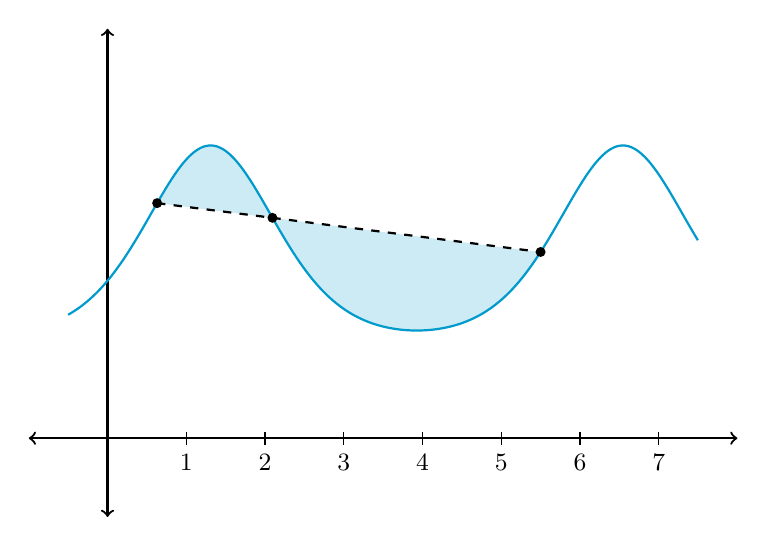
\begin{tikzpicture}
    % interval
    \def\xstart{0.63}
    \def\xend{5.5}
    \pgfmathdeclarefunction{f}{1}{%
    \pgfmathparse{1 + exp(sin(1.2 * #1 r))}%
    }
    \pgfmathparse{f(\xstart)} \let\fstart\pgfmathresult
    \pgfmathparse{f(\xend)}   \let\fend\pgfmathresult
    \pgfmathsetmacro{\m}{(\fend-\fstart)/(\xend-\xstart)}
    % (optional) declare g(x) if you want to call it
    \pgfmathdeclarefunction{g}{1}{%
    \pgfmathparse{\m*(#1-\xstart) + \fstart}%
    }

    \def\maxX{7}
    \def\maxY{5}
    \draw[<->, thick] (-1,0) -- (\maxX+1,0);
    \draw[<->, thick] (0,-1) -- (0,\maxY+0.2);
    \foreach \i in {1,...,7} {
    \draw (\i,0.08) -- (\i,-0.08) node[below] {\small $\i$};
    }
    \fill[DeepSkyBlue3!20] 
    (\xstart,\fstart)
    plot[domain=\xstart:\xend, samples=240, smooth] (\x,{f(\x)})
    -- (\xstart,\fstart) -- cycle;

    \draw[thick, DeepSkyBlue3] 
    plot[domain=-0.5:\maxX+0.5, samples=600, smooth] (\x,{f(\x)});
    %Bounding line
    \draw[dashed, thick] (\xstart,\fstart) -- (\xend,\fend);

    \foreach \i in {0.63, 2.09484, 5.5} {
      \fill (\i,{f(\i)}) circle (1.8pt);
    }

\end{tikzpicture}

\noindent La función no es convexa en $[0,6]$, pero sí en $[2,6]$.
\end{center}

\vspace{4mm} Podemos considerar definiciones distintas de convexidad según exijamos o no que la desigualdad sea estricta.

\vspace{6mm}
\result{Los \texorpdfstring{$\mathcal{L}_p(X)$}{L\_p(X)} son espacios vectoriales}
\hspace{3mm} Para $1 \leq p \leq \infty$, $\mathcal{L}_p(X)$ es un espacio vectorial.
\vspace{6mm} \newline \dem Distinguiremos varios casos:
\vspace{2mm} \newline \noindent $\bullet$ Caso $p=1$: \hyperref[result:2.2.4]{ya se ha demostrado}.
\vspace{2mm} \newline \noindent $\bullet$ Caso $p= \infty$:
\begin{adjustwidth}{0.07\textwidth}{}
    \vspace{-4mm} Sea $f \in \mathcal{L}_\infty(X)$, sea $\lambda \in \R$. Veamos $\lambda f \in \mathcal{L}_\infty(X)$.
    \vspace{2mm} \newline Si $\lambda = 0$, $\lambda f \equiv 0 \in \mathcal{L}_\infty(X)$.
    \vspace{2mm} \newline Sea $\lambda \in \R \setminus \{0\}$. Como $f \in \mathcal{L}_\infty(X)$, $\exists$ $M \in \Sigma$ con $\mu(M) = 0$ tal que:
    $$X \setminus M = \{x \in X : |f(x)|\leq ||f||_\infty\} = \{x \in X : |\lambda f(x)|\leq |\lambda|\cdot ||f||_\infty\}$$
    Tenemos que $\lambda f \in \mathcal{L}_\infty(X)$ por definición.

    \vspace{5mm} Sean $f,g\in \elep{\infty}{X}$, veamos que $f+g\in \elep{\infty}{X}$:
    \vspace{2mm} \newline Por definición, $\exists \hspace{1mm} M,N \in \Sigma$ con $\mu(M) = \mu(N) = 0$ tales que: \\[-3ex]
    \begin{align*}
        X \setminus M = \{x \in X : |f(x)| \leq ||f||_\infty\} &&
        X \setminus N = \{x \in X : |g(x)| \leq ||g||_\infty\} 
    \end{align*}
    Entonces, dado $x \in X \setminus(M \cup N)$ cualquiera, se cumple:
    $$|f(x) + g(x) | \leq |f(x)| + |g(x)| \leq ||f||_{\infty} + ||g||_{\infty} < \infty $$
    Como $\mu(M \cup N) = 0$, tenemos $f+g\in \elep{\infty}{X}$ por definición.
\end{adjustwidth}
\vspace{6mm} \noindent $\bullet$ Caso $1 < p < \infty$:
\begin{adjustwidth}{0.07\textwidth}{}
    Sean $\lambda \in \R, f \in \elep{p}{X}$. Veamos que $\lambda f \in \elep{\infty}{X}$.
    $$\int_{X}|\lambda f(x)|^p\,d\mu(x) = |\lambda|^p \cdot \int_{X}|f(x)|^p\,d\mu(x) = |\lambda|^p \cdot ||f||_p^p < \infty$$
    Se cumple por definición.

    \vspace{4mm} Sean $f,g \in \elep{p}{X}$. Veamos que $f+g\in \elep{p}{X}$:
    \begin{flalign*}
        \int_{X}&|f(x)+p(x)|\,d\mu(x) = \int_{X} \Big|\hspace{1mm} \underbrace{\frac{1}{2}}_\lambda\cdot 2 \cdot f(x)+ \underbrace{\frac{1}{2}}_{1-\lambda}\cdot 2 \cdot g(x)\hspace{1mm} \Big|^p\,d\mu(x) = (*)
    \end{flalign*}
    La función $h(t) = |t|^p$ es convexa en $[0,+\infty]$ para $p > 1$. Por tanto,
    \begin{flalign*}
        (*) &\leq \int_{X}\frac{1}{2}\left|2f(x)\right|^p + \frac{1}{2} |2g(x)|^p\,d\mu(x) = 2^{p-1}\cdot \int_{X}|f(x)|^p\,d\mu(x) + 2^{p-1} \cdot \int_{X}|g(x)|^{p}\,d\mu(x) = &&\\
        &= 2^{p-1}\left(\int_{X}|f(x)|^p\,d\mu(x) + \int_{X}|g(x)|^p\,d\mu\right) = 2^{p-1}\big(||f||_p^p + ||g||_p^p\big) < \infty
    \end{flalign*}
    Se cumple por definición.
\end{adjustwidth}

\vspace{6mm}
\result{Conjugado \texorpdfstring{$p^*$}{p*}}
\hspace{3mm} Para cada $p \in [1, +\infty]$, denotaremos como $p^*$ al único número en $\overline{\R}$ que verifica:
$$\frac{1}{p} + \frac{1}{p^*} = 1$$
Solo hay un único número en todo $\overline{\R}$ que verifica esto, pero ha de estar necesariamente en $(1, \infty)$:
$$\frac{1}{p} + \frac{1}{p^*} = 1 \Rightarrow p^* = \frac{1}{1 - \frac{1}{p}} = \frac{p}{p-1} \overset{p\in[1,\infty]}{\in} (1, \infty)$$
\indent Estas son algunas de las propiedades de este conjugado (claras por la definición):
\begin{align*}
    (p^*)^* = p && p + p^* = p\cdot p^* = \frac{p^2}{p-1} && p^* = \frac{p}{p-1} && p^*(p-1) = p
\end{align*}

\vspace{6mm}
\result{Desigualdad de Hölder}
\hspace{3mm} Sean $f \in \elep{p}{X}$, $g \in \elep{p^*}{X}$. Entonces, se cumple:
\begin{align*}
    f\cdot g \in \elep{1}{X} && ||f\cdot g||_1 \leq ||f||_p \cdot ||g||_{p^*}
\end{align*}
\vspace{3mm} \dem
\vspace{2mm} \newline $\bullet$ Caso $p = 1, p^* = \infty$:
\begin{adjustwidth}{0.07\textwidth}{}
    \vspace{2mm} Como $g \in \elep{\infty}{X}$, $\exists$ $M \in \Sigma$ con $\mu(M) = 0$ tal que
    $$X \setminus M = \{x \in X : |g(x)| \leq ||g||_\infty\}$$
    Por tanto, ha de cumplirse:
    \begin{flalign*}
      \int_{X}&=|f\cdot g|\,d\mu = \int_{X \setminus M}|f(x)| \cdot |g(x)|\,d\mu(x) \leq \int_{X \setminus M}|f(x)| \cdot ||g||_\infty\,d\mu = &&\\
      &= ||g||_\infty \cdot \int_{X \setminus M}|f(x)|\,d\mu(x) = ||g||_\infty \cdot ||f||_1 < \infty
    \end{flalign*}
    Se cumple por definición.    
\end{adjustwidth}

\vspace{6mm} \noindent $\bullet$ Caso $1 < p < \infty$. Hay que estudiar dos posibles escenarios:
\vspace{2mm} \newline \indent a) Si $||f||_p = 0$ ó $||g||_{p^*} = 0$ (pudiendo darse ambas). Supongamos sin pérdida de generalidad que $||f||_p = 0$:
\newpage
\begin{adjustwidth}{0.07\textwidth}{}
    \vspace{2mm} $||f||_p = 0 \Rightarrow = \int_{X}|f|^p\,d\mu(x) = 0 \overset{\hyperref[result:2.1.17]{2.1.17}}{\Rightarrow} |f|^p \muae 0 \Rightarrow f \muae 0$.
    \vspace{2mm} \newline De este modo, $f \cdot g \muae 0 \Rightarrow |f\cdot g| \muae 0 \overset{\hyperref[result:2.1.17]{2.1.17}}{\Rightarrow} 0 = \int_{X}\,|f\cdot g|d\mu = ||f\cdot g||_1$.
\end{adjustwidth}

\vspace{6mm} b) \noindent Supongamos ahora que $||f||_p \neq 0 \neq ||g||_{p^*}$. Así,
\begin{adjustwidth}{0.07\textwidth}{}
    \vspace{3mm} Definimos los siguientes conjuntos auxiliares: \\[-3ex]
    \begin{align*}
        A := \{x \in X : f(x) = 0\} \in \Sigma &&  B := \{x \in X : g(X) = 0\} \in \Sigma
    \end{align*}
    Por cómo los hemos definido,
    $$\int_{X}\frac{|f(x)|}{||f||_p}\cdot \frac{|g(x)|}{||g||_{p^*}}\,d\mu(x) = \int_{X \setminus(A\cup B)}\frac{|f(x)|}{||f||_p} \cdot \frac{|g(x)|}{||g||_{p^*}}\,d\mu(x) = (*_1)$$
    Al tratarse de cantidades positivas, para cada $x \in X \setminus (A\cup B)$, existen $\xi_x, \zeta_x \in (0, \infty)$ tales que:
    \begin{align*}
      \frac{|f(x)|}{||f||_p} = e^{\frac{\xi_x}{p}} = \exp\left(\frac{\xi_x}{p}\right) &&\frac{|g(x)|}{||g||_{p^*}} = e^{\frac{\zeta_x}{p^*}} = \exp\left(\frac{\zeta_x}{p^*}\right)
    \end{align*}
    Sustituyendo en la expresión anterior:
    \begin{flalign*}
        (*_1) = \int_{X \setminus (A\cup B)}\hspace{-3mm} \exp\left(\frac{\xi_x}{p}\right) \cdot \exp\left(\frac{\zeta_x}{p^*}\right)\,d\mu(x) = \int_{X \setminus(A \cup B)}\hspace{-3mm} \exp\left(\frac{1}{p}\xi_x + \frac{1}{p^*}\zeta_x\right)\,d\mu(x)
    \end{flalign*}
    La función exponencial es convexa. Tomando $\lambda = \frac{1}{p}$, $1-\lambda = \frac{1}{p^*}$, tenemos:
    \begin{flalign*}
        (*_1) \leq \hspace{-3mm} \mathop{\int}_{X\setminus(A\cup B)}\hspace{-3mm} \frac{1}{p}\exp(\xi_x) + \frac{1}{p^*}\exp(\zeta_x)\,d\mu(x) = \frac{1}{p} \hspace{-5mm} \mathop{\int}_{X \setminus(A \cup B)}\hspace{-5mm} \exp(\xi_x)\,d\mu(x) + \frac{1}{p^*} \hspace{-5mm} \mathop{\int}_{X \setminus (A\cup B)}\hspace{-5mm} \exp(\zeta_x)\,d\mu(x) = (*_2)
    \end{flalign*}
    Deshacemos el cambio de variable y comparamos con la definición de $||\cdot||_p$ y de $||\cdot||_{p^*}$,
    \begin{flalign*}
        (*_2) &= \frac{1}{p} \hspace{-5mm}\mathop{\int}_{X \setminus(A\cup B)}\hspace{-3mm} \frac{|f(x)|^p}{||f||_p^p}\,d\mu(x) + \frac{1}{p^*} \hspace{-5mm} \mathop{\int}_{X \setminus(A \cup B)}\hspace{-3mm} \frac{|g(x)|^{p^*}}{||g||^{p^*}_{p^*}}\,d\mu(x) = &&\\
        &= \frac{1}{p \cdot ||f||^p_p} \cdot {\int}_{X}|f(x)|^p\,d\mu(x) + \frac{1}{p^* \cdot ||g||^{p^*}_{p^*}} \cdot {\int}_{X} \hspace{2mm} |g(x)|^{p^*}\,d\mu(x) = \\
        &= \frac{1}{p \cdot ||f||^p_p} \cdot ||f||^p_p + \frac{1}{p^* \cdot ||g||^{p^*}_{p^*}} \cdot ||g||^{p^*}_{p^*} = \frac{1}{p} + \frac{1}{p^*} = 1
    \end{flalign*}
    \newpage \noindent Sustituimos para resolver el problema inicial:
    \begin{flalign*}
        \int_{X}\frac{|f(x)|}{||f||_p}\cdot \frac{|g(x)|}{||g||_{p^*}}\,d\mu(x) \leq 1
        \Rightarrow \int_{X}|f(x) \cdot g(x)|\,d\mu(x) \leq ||f||_p \cdot ||g||_{p^*} < \infty
    \end{flalign*}
\end{adjustwidth}

\vspace{6mm} \result{Desigualdad de Minkowski}
\hspace{3mm} Sea $1 \leq p \leq \infty$. Sean $f,g \in \elep{p}{X}$. Entonces, $||f+g||_p \leq ||f||_p + ||g||_p$.
\vspace{4mm} \newline \dem Hemos de distinguir tres casos.
\vspace{2mm} \newline $\bullet$ Caso $p=1$: \hyperref[result:2.1.9]{ya ha sido probado}.
\vspace{2mm} \newline $\bullet$ Caso $p=\infty$:
\begin{adjustwidth}{0.07\textwidth}{}
    \vspace{2mm} Por ser $f,g \in \elep{\infty}{X}$, sabemos $\exists$ $M,N \in \Sigma$ con $\mu(M) = \mu(N) = 0$ tales que: \\[-3ex]
    \begin{align*}
        X \setminus M = \{x \in X : |f(x)| \leq ||f||_\infty\} && X \setminus N = \{x \in X : |g(x)| \leq ||g||_\infty\}
    \end{align*}
    Entonces, dado $x \in X \setminus (M \cup N)$, se cumple:
    $$|f(x) + g(x)| \leq |f(x)| + |g(x)| \leq ||f||_\infty + ||g||_\infty $$
    Como $\mu(M\cup N) = 0$. Recordando la (\hyperref[result:3.1.4]{notación 3.1.4}), tenemos:
    $$||f||_\infty + ||g||_\infty \in A_{f+g} \Rightarrow ||f+g||_\infty = \min A_{f+g} \leq ||f||_\infty + ||g||_\infty$$
\end{adjustwidth}
\vspace{4mm} $\bullet$ Caso $1 < p < \infty$:
\begin{adjustwidth}{0.07\textwidth}{}
    \vspace{-4ex}
    \begin{flalign*}
        &||f+g||_p^p = \int_{X}|f+g|^p\,d\mu = \int_{X}|f+g| \cdot |f+g|^{p-1}\,d\mu \leq &&\\[2ex]
        &= \hspace{2mm} \int_{X}\underbracket{\hspace{0.5mm} |f| \hspace{0.5mm}}_{\elep{p}{X}} \cdot \underbracket{\hspace{0.5mm}|f+g|^{p-1} \hspace{0.5mm}}_{\elep{p^*}{X}}\,d\mu
            + \int_{X}\underbracket{\hspace{0.5mm} |g| \hspace{0.5mm}}_{\elep{p}{X}} \cdot \underbracket{\hspace{0.5mm}|f+g|^{p-1} \hspace{0.5mm}}_{\elep{p^*}{X}}\,d\mu = (*)
    \end{flalign*}
    Por las \hyperref[result:3.2.3]{propiedades de $p^*$}, tenemos que:
    $$\int_{X}\left(|f + g|^{p-1}\right)^{p^*}\,d\mu = \int_{X}|f + g|^{p^*(p-1)}\,d\mu = \int_{X}|f+g|^p\,d\mu = ||f+g||_p^p < \infty$$
    Podemos aplicar la \hyperref[result:3.2.4]{Desigualdad de Hölder} a ambos sumandos: \newpage
    \begin{flalign*}
        (*) &\leq ||f||_p \cdot \Big| \Big| |f+g|^{p-1} \Big| \Big{|}_{p^*} + ||g||_p \cdot \Big| \Big| |f+g|^{p-1} \Big| \Big{|}_{p^*} = (||f||_p + ||g||_p) \cdot \Big| \Big| |f+g|^{p-1} \Big| \Big{|}_{p^*} = &&\\[2ex]
        &= (||f||_p + ||g||_p) \cdot \left(\int_{X}|f+g|^{p^*(p-1)}\,d\mu\right)^\frac{1}{p^*} = (||f||_p + ||g||_p) \cdot \left(||f+g||_p^p\right)^\frac{1}{p^*} = \\[2ex]
        &= (||f||_p + ||g||_p) \cdot ||f+g||_p^{p-1}
    \end{flalign*}

    \vspace{2mm} \noindent Así, $||f+g||_p^p \leq (*) \leq (||f||_p + ||g||_p) \cdot ||f+g||_p^{p-1}$. Despejando,
    $$||f+g||_p^{p-(p-1)} = ||f+g||_p \leq ||f||_p + ||g||_p $$
\end{adjustwidth}

\vspace{6mm}
\result{Definición de espacio vectorial seminormado}
\hspace{3mm} Un $K$-espacio vectorial $V$ se dice ``seminormado'' si existe una aplicación \newline $||\cdot|| : V \longrightarrow [0,+\infty)$ (llamada ``seminorma de $V$'') que cumple las siguientes condiciones:
\begin{enumerate}[label=\roman*)]
    \item $||\lambda v|| = |\lambda| \cdot ||v||$ $\forall \hspace{1mm} \lambda \in K$ $\forall \hspace{1mm} v \in V$.
    \item $||x+y|| \leq ||x|| + ||y||$ $\forall \hspace{1mm} x,y \in V$.
\end{enumerate}
Nótese que como consecuencia de $(i)$ se cumple $||0_V|| = 0$.

\vspace{4mm} En vista del \hyperref[result:3.2.5]{resultado anterior}, es claro que los $\elep{p}{X}$ son espacios vectoriales seminormados para $1 \leq p \leq \infty$.

\newpage
\chapter{Paso a conjuntos cocientes \texorpdfstring{$L_p$}{L\_p}}
\result{Conjunto cociente dado por subespacio vectorial}
\hspace{3mm} Sea $V$ un espacio vectorial. Sea $N \leq V$ un subespacio vectorial. Podemos definir una relación de equivalencia en $V$ como sigue:
$$x \sim y \iff x - y \in N \hspace{4mm} \forall x,y \in V $$
Veamos que es en efecto una relación de equivalencia.
\vspace{4mm} \newline \noindent $\bullet$ Relfexividad:
\begin{adjustwidth}{0.07\textwidth}{}
    \vspace{2mm}
    Por ser $N$ un subespacio vectorial, tenemos $0_V = 0_N \in N$.
    \vspace{2mm} \newline De este modo, sea $x\in V$ cualquiera, $x-x = 0_V \in N$.
\end{adjustwidth}
\vspace{4mm} \noindent $\bullet$ Simetría:
\begin{adjustwidth}{0.07\textwidth}{}
    Sean $x,y \in V$ tales que $x \sim y$, veamos que $y \sim x$.
    \vspace{2mm} \newline Por definición, $x-y \in N \Rightarrow -(x-y) = y -x \in N$.
    \vspace{2mm} \newline Se tiene el ser $N$ un espacio vectorial.
\end{adjustwidth}
\vspace{4mm} \noindent $\bullet$ Transitividad:
\begin{adjustwidth}{0.07\textwidth}{}
    Sean $x,y,< \in V$ tales que $x \sim y$, $\hspace{1mm} y \sim z$. Veamos que $x \sim z$.
    \vspace{2mm} \newline Por definición, $x-y \in N$, $\hspace{1mm} y- z \in N$.
    \vspace{2mm} \newline Así, $x-z = (x-y) - \underbracket{(z-y)}_{\in N} \in N$.
\end{adjustwidth}
\vspace{2mm} \indent Es muy común denotar al espacio cociente resultante como ${V}/{N}$ en lugar de ${V}/{\sim}$. De manera similar, sus elementos suelen denotarse como $v + N$ en lugar de $[v]_{\sim}$.
\vspace{4mm} \newline \indent Además, respeta la estructura de espacio vectorial. Es decir, sean $x, y \in V$, $\alpha, \beta \in K$; se cumple:
$$(\alpha x + \beta y) + N = \alpha(x+N) + \beta(y+N) $$

\vspace{3mm} \noindent
Esto se debe a que $\forall \hspace{1mm} z \in V$, $\forall \lambda \in K$,
$$||x-y|| = 0 \iff ||\lambda x -\lambda y|| = 0$$
$$||x-y||= 0 \iff ||(x+z) - (y+z)||= 0$$

\vspace{6mm}
\result{Convertir un espacio seminormado en uno normado}
\hspace{3mm} Sea $(V, ||\cdot||)$ un $K$-espacio vectorial seminormado, veamos cómo obtener un espacio vectorial normado a partir de él. Veamos que el siguiente conjunto es un subespacio vectorial:
$$ N = \{v \in V : ||v|| = 0\}$$
Sean $u,v \in N$, sean $\alpha, \beta \in K$, se cumple:
$$ ||\alpha u + \beta v|| \leq ||\alpha u ||+ ||\beta v|| = |\alpha|\cdot ||u|| + |\beta|\cdot ||v|| = 0 + 0 = 0$$
Utilizaremos este subespacio para el paso a cocientes.

\vspace{2mm} Proponemos la siguiente aplicación como candidata a norma:
\begin{align*}
    ||\cdot||' : V/N \to [0, \infty) && v+N \mapsto ||v+N||' = ||v||
\end{align*}
En primer lugar, veamos que está bien definida. Sean $u,v\in V$ tales que $u \sim v$, buscamos ver $||u||= ||v||$:
$$||u|| = ||u+0_v|| = ||(u-v) + v||\leq ||u-v|| + ||v|| \Rightarrow ||u|| - ||v|| \leq ||u-v|| = 0$$
Análogamente, $||v||- ||u|| \leq ||u-v|| = 0$. Queda ver que $||\cdot||'$ es una norma.


\begin{enumerate}[label=\roman*)]
    \item Sean $u\in V$, $\lambda \in K$,
    $$||\lambda(u+N)||' = ||(\lambda u) + N ||' = ||\lambda x||= |\lambda| \cdot ||u|| = |\lambda|\cdot ||u+N||'$$

    \item Sean $u,v\in V$,
    $$||(u+v)+N||' = ||(u+N) + (v+N)||' = ||u+v||\leq||u||+||v||= ||u+N||'+||v+N||'$$

    \item Sea $u\in V$ tal que $||u+N||' = 0$,
    $$||u+N||' = 0 \Rightarrow ||u||= 0 \Rightarrow u \in N \Rightarrow u + N = N = 0_{V/N}$$
\end{enumerate}

\vspace{4mm} \noindent \nota Habitualmente, solemos escribir $(V/N, ||\cdot||)$ en lugar de $(V/N, ||\cdot||')$.

\newpage
\result{Unicidad del conjunto \texorpdfstring{$N$}{N} en los \texorpdfstring{$\mathcal{L}_p(X)$}{L\_p(X)}}
\hspace{3mm} Sea $1 \leq p \leq \infty$, se cumple:
$$N_p := \{f \in \mathcal{L}_p(X) : ||f||_p = 0\} = N := \{f: X \to \R \text{ medible con }f \muae 0\}$$

\vspace{2mm} \dem Distinguiremos varios casos.
\vspace{2mm} \newline $\bullet$ Para $p = \infty$:
\begin{adjustwidth}{0.07\textwidth}{}
    $$||f||_\infty = 0 \iff \{x \in X : |f(x)| \leq 0\} \muae X \iff f \muae 0$$
\end{adjustwidth}

\vspace{2mm}
\noindent $\bullet$ Caso $1 \leq p < \infty$:
\begin{adjustwidth}{0.07\textwidth}{}
    $$||f||_p = \left(\int_{X}|f(x)|^p\,d\mu(x)\right)^\frac{1}{p} = 0 \iff |f(x)|^p \muae 0 \iff f \muae 0$$
\end{adjustwidth}

\vspace{6mm}
\result{Definición de espacios \texorpdfstring{$L_p$}{L\_p}}
\hspace{3mm} Para cada $1 \leq p \leq \infty$, definimos siguiente espacio vectorial normado:
$$L_p(X,\Sigma, \mu) := \Big(\mathcal{L}_p(X,\Sigma, \mu)/N, ||\cdot||_p\Big)$$
\indent Cuando el contexto sea claro, escribiremos simplemente $L_p(X)$. Además, denotaremos $f \in L_p(X)$ en lugar de $f+N \in L_p(X)$ ó $[f]_\sim \in L_p(X)$.
\vspace{2mm} \newline \indent Consideramos que $f = g$ en $L_p(X, \Sigma, \mu)$ significa $f(x) \muae g(x)$ como funciones.

\vspace{6mm}
\result{Espacios \texorpdfstring{$\ell_p$}{l\_p} como espacios \texorpdfstring{$L_p$}{L\_p}}
\hspace{3mm} Estudiemos el caso particular $L_p(\N, \mathcal{P}(\N), m)$ para $m$ \hyperref[result:1.1.6]{medida de contar}.
\vspace{2mm} \newline \indent Sea $s \in \mathcal{L}_p(\N , \mathcal{P}(\N), m)$, tenemos que $s$ es una función de la forma:
\begin{align*}
    s : \N \longrightarrow \R && n \mapsto s(n)
\end{align*}
De modo que $s \equiv (x_n)_{n\in \N}$. Por tanto,
$$||s||_p = \left(\int_{\N}|s(n)|^p\,dm(n)\right)^\frac{1}{p} = \left(\sum_{n=1}^{\infty}|x_n|^p\right)^\frac{1}{p} \overset{s \in \mathcal{L}_p}{<} \infty$$
Se corresponden con los espacios $\ell_p$ estudiados en Análisis Matemático 2. Además, en este caso, el conjunto $N$ contiene únicamente a la sucesión nula $0_{\ell_p} \equiv 0$.

\vspace{6mm}
\result{Teorema de Riesz-Fisher}
\hspace{3mm} Sea $1 \leq p \leq \infty$. Sea $(f_n)_{n\in\N} \subseteq \mathcal{L}_p(X)$  sucesión de Cauchy en $L_p(X)$. Entonces, existen $(k_n)_n \subseteq (n)_n$ sucesión creciente de naturales, y $f \in \mathcal{L}_p(X)$ que verifican:
\begin{enumerate}[label=\roman*)]
    \item $f_{k_n}(x) \xrightarrow{n\to\infty} f(x)$ en casi todo punto ($\mu$-a.e.)
    \item $||f_n - f||_p \xrightarrow{n\to\infty}0$
    \item Para el caso $p = \infty$, podemos tomar $(k_n)_n = (n)_n$
\end{enumerate}
Como consecuencia, $L_p(X, \Sigma, \mu)$ es un espacio de Banach.

\vspace{4mm} \dem Veremos dos casos.
\vspace{2mm} \newline $\bullet$ Caso $1 \leq p < \infty$:
\begin{adjustwidth}{0.07\textwidth}{}
    Como $(f_n)_n$ es de Cauchy en $L_p(X)$. Para cada $n \in \N$ podemos afirmar que existe cierto $k_n \in \N$ tal que:
    $$ ||f_k - f_{k_n}||_p < \frac{1}{2^n} \hspace{2mm} \forall \hspace{1mm} k \geq k_n$$
    En particular, $|f_{k_{n+1}} - f_{k_n}||_p < \frac{1}{2^n}$ $\forall \hspace{1mm} n \in \N$.
    \vspace{2mm} \newline Consideramos las siguientes funciones medibles:
    \begin{align*}
        g_n(x) := \sum_{m=1}^{n}|f_{k_{m+1}}(x) - f_{k_m}(x)| &&
        g(x) := \sum_{n=1}^{\infty}|f_{k_{n+1}}(x) - f_{k_n}(x)|
    \end{align*}
    Veamos que $g$ es sumable. Como es suma de términos no negativos, podemos aplicar el Teorema de Convergencia Monótona:
    \begin{flalign*}
        \int_{X}&g(x)^p\,d\mu(x) \overset{TCM}{=} \lim_{n} \int_{X}g_n(x)^p\,d\mu(x) = \lim_{n} \left| \left|\sum_{m=1}^{n}|f_{k_{m+1}}(x) - f_{k_m}(x)| \right| \right|_p^p \overset{\text{continuidad}}{=} \\
        &= \left(\lim_n \left|\left|\sum_{m=1}^{n}|f_{k_{m+1}}(x) - f_{k_{m}}(x)|\right|\right|_p\right)^p \overset{D.T.}{\leq} \left(\lim_n \sum_{m=1}^{n}||f_{k_{m+1}} - f_{k_m}||_p\right)^p \leq
    \end{flalign*}
    \newpage
    \begin{flalign*}
        \hspace{6mm} \leq \left(\lim_{n}\sum_{m=1}^{n}\frac{1}{2^n}\right)^p < \infty &&
    \end{flalign*}
    Tenemos que $g(x) < \infty$ $\mu$-a.e. al ser sumable. Por tanto, para el siguiente conjunto, \\[-3ex]
    $$ A := \{x \in X : g(x) = \infty\} \in \Sigma$$
    tenemos que $\mu(A) = 0$. Sea $x \in X \setminus A$, tenemos $g(x) < \infty$ luego ha de cumplirse: \\[-3ex]
    $$g(x) := \sum_{n=1}^{\infty}f_{k_{n+1}}(x) - f_{k_n}(x) < \infty$$
    Al ser una serie telescópica, esto implica que $\exists \lim_{n}f_{k_n}(x) < \infty$.
    \newline Definimos la función candidata a límite:
    \begin{align*}
        f: X \longrightarrow \R &&
        x \longmapsto f(x) := \begin{cases}
            \mlim{n} \hspace{1mm} f_{k_n}(x) &\text{ si } x \in X \setminus A\\
            0 &\text{ si } x \in A
        \end{cases}
    \end{align*}
    Tenemos garantizado que $f_{k_n}(x) \xrightarrow{n\to\infty}f(x)$ en $X \setminus A$ con $\mu(A) = 0$ luego hemos demostrado ya el primer apartado. Queda ver que se cumple el segundo.
    \begin{flalign*}
        \int_{X}&|f - f_{k_n}|^p\,d\mu = \int_{X \setminus A} \linf{m} \hspace{1mm} |f_{k_m} - f_{k_n}|^p\,d\mu \overset{\hyperref[result:2.1.13]{Fatou}}{\leq} \linf{m} \int_{X \setminus A}|f_{k_m}(x) - f_{k_n}(x)|\,d\mu(x) = \\[1.5ex]
        &= \left(\linf{m}||f_{k_m}-f_{k_n}||_p\right)^p \leq \left(\frac{1}{2^n}\right)^p
    \end{flalign*}
    \vspace{4mm} \newline \indent En particular, tomando $k_n = k_1$,
    $$\int_{X}|f(x) - f_{k_1}(x)|^p \,d\mu(x) < \infty \Rightarrow f - f_{k_1} \in \mathcal{L}_p(X)$$
    Como $f_{k_1} \in \mathcal{L}_p(X)$, al ser un espacio vectorial, $f \in \mathcal{L}_p(X)$.
    \vspace{4mm} \newline Además, $||f-f_{k_n}||_p^p \leq \frac{1}{2^{np}} \xrightarrow{n\to\infty}0$.
    \vspace{3mm} \newline Es decir, $f_{k_n} \xrightarrow{n\to\infty}f$ en $L_p(X)$.
    \vspace{3mm} \newline Como $(f_n)_n$ es de Cauchy en $L_p(X)$, $||f_n - f||_p \xrightarrow{n\to\infty}0$.
\end{adjustwidth}

\newpage
\noindent $\bullet$ Caso $p=\infty$:
\begin{adjustwidth}{0.07\textwidth}{}
    \vspace{2mm} Por hipótesis, tenemos $(f_n)_n$ de Cauchy en $L_\infty(X)$ luego
    $$ \forall \hspace{1mm} \varepsilon > 0 \hspace{2mm} \exists \hspace{1mm} n_\varepsilon \in \N \text{ tal que } ||f_n - f_m||_\infty < \varepsilon \hspace{3mm} \forall \hspace{1mm} n,m \geq n_\varepsilon$$
    Para cada par $(n,m) \in \N^2$ definimos el siguiente conjunto auxiliar:
    $$A_{n,m} := \Big\{x \in X : |f_n(x) - f_m(x)| \leq ||f_n - f_m||_\infty \Big\} $$
    Así, para $B_{n,m} := X \setminus A_{n,m} \in \Sigma$ tenemos $\mu(B_{n,m})=0$.
    \vspace{3mm} \newline Y por tanto, $B := \smallcup_{(n,m)\in\N^2} B_{n,m} \in \Sigma$ con $\mu(B) = 0$.
    \vspace{4mm} \newline Sea $\varepsilon > 0$. Tenemos:
    $$ \forall \hspace{1mm} x \in X \setminus B, \hspace{2mm} \forall \hspace{1mm} n,m \geq n_\varepsilon : |f_n(x) - f_m(x)| \leq ||f_n - f_m||_\infty < \varepsilon$$
    Tenemos que para todo $x \in X \setminus B$ la sucesión $(f_n(x))_n$ es de Cauchy en $\R$.
    \vspace{2mm} \newline Al ser un espacio métrico completo, converge en $\R$. Podemos definir:
    \begin{align*}
        f: X \longrightarrow \R &&
        x \longmapsto f(x) := \begin{cases}
            \mlim{n} \hspace{1mm} f_{n}(x) &\text{ si } x \in X \setminus B\\
            0 &\text{ si } x \in B
        \end{cases}
    \end{align*}
    Dados $x \in X \setminus B$, $m \geq n_\varepsilon$, se cumple:
    $$|f(x) - f_m(x)| = \lim_n |f_n(x) - f_m(x)| \overset{n \geq n_\varepsilon}{\leq} \varepsilon$$
    Tenemos $f = (f- f_m) + f_m \in \mathcal{L}_\infty(X)$, luego $f \in \mathcal{L}_\infty(X)$ al ser un espacio vectorial .
    \vspace{3mm} \newline Además, $\forall \hspace{1mm} m \geq n_\varepsilon, ||f-f_m||_\infty < \varepsilon$.
    \vspace{3mm} \newline Así, $f_m \xrightarrow{m\to\infty}f$ en $L_\infty(X)$.
\end{adjustwidth}
\end{document}